\documentclass[11pt,a4paper,oneside]{report}

\usepackage{fontspec}
\usepackage[brazilian]{babel}
\usepackage[top=2.3cm,bottom=2.3cm,left=2.1cm,right=2.1cm,headheight=14pt]{geometry}
\usepackage{amsmath,amssymb,amsfonts}
\usepackage{graphicx}
\usepackage{booktabs}
\usepackage{array}
\usepackage{longtable}
\usepackage{xcolor}
\usepackage{fancyhdr}
\usepackage{titlesec}
\usepackage{tikz}
\usetikzlibrary{arrows.meta,positioning,shapes.geometric,calc}
\usepackage[most]{tcolorbox}
\usepackage[numbers,sort&compress]{natbib}
\usepackage[plainpages=false,pdfpagelabels=true]{hyperref}

\definecolor{abNavy}{HTML}{0F4C81}
\definecolor{abViolet}{HTML}{6D28D9}
\definecolor{abEmerald}{HTML}{059669}
\definecolor{abCrimson}{HTML}{B91C1C}
\definecolor{abSlate}{HTML}{334155}
\definecolor{abBgBlue}{HTML}{EFF6FF}
\definecolor{abBgGold}{HTML}{FEFCE8}
\definecolor{abBgGreen}{HTML}{ECFDF5}
\definecolor{abGold}{HTML}{CA8A04}

\hypersetup{
  colorlinks=true,
  linkcolor=abNavy,
  citecolor=abViolet,
  urlcolor=abNavy,
  pdftitle={AlphaBuilder v4.0: Do Calculo Variacional ao Self-Play Fisico com Phys-UViT 3D},
  pdfauthor={Projeto AlphaBuilder}
}

\pagestyle{fancy}
\fancyhf{}
\renewcommand{\chaptermark}[1]{\markboth{\thechapter.\ #1}{}}
\fancyhead[L]{\footnotesize\color{abSlate}\textit{AlphaBuilder v4.0}}
\fancyhead[R]{\footnotesize\color{abNavy}\nouppercase{\leftmark}}
\fancyfoot[C]{\small\thepage}
\renewcommand{\headrulewidth}{0.4pt}
\renewcommand{\footrulewidth}{0pt}

\titleformat{\chapter}[display]
  {\normalfont\bfseries\color{abNavy}\raggedright}
  {\large\MakeUppercase{\chaptertitlename}~\thechapter}
  {0.35em}
  {\LARGE}
\titlespacing*{\chapter}{0pt}{-10pt}{14pt}
\titleformat{\section}
  {\normalfont\Large\bfseries\raggedright}
  {\thesection}{0.6em}{}
\titleformat{\subsection}
  {\normalfont\large\bfseries\raggedright}
  {\thesubsection}{0.6em}{}

\newtcolorbox{eurekabox}[1]{
  enhanced,
  colback=abBgBlue,
  colframe=abNavy,
  boxrule=0.9pt,
  arc=3pt,
  fonttitle=\bfseries\small,
  title={Momento Eureka — #1},
  coltitle=white,
  colbacktitle=abNavy
}

\newtcolorbox{mathbox}[1]{
  enhanced,
  colback=abBgGreen,
  colframe=abEmerald,
  boxrule=0.8pt,
  arc=3pt,
  fonttitle=\bfseries\small,
  title={Síntese Matemática e Mecânica — #1},
  coltitle=white,
  colbacktitle=abEmerald
}

\newtcolorbox{notabox}[1]{
  enhanced,
  colback=abBgGold,
  colframe=abGold,
  boxrule=0.9pt,
  arc=3pt,
  fonttitle=\bfseries\small,
  title={Nota de Rigor Científico — #1},
  coltitle=black,
  colbacktitle=abGold!35!white
}

\graphicspath{{figures/}}
\setlength{\parskip}{0.55em}
\setlength{\parindent}{0pt}
\setcounter{tocdepth}{2}
\emergencystretch=2.5em
\sloppy
\raggedbottom

\begin{document}
\pagenumbering{roman}

\begin{titlepage}
\centering
\vspace*{1.4cm}
{\color{abNavy}\rule{\textwidth}{1.5pt}}\\[0.9cm]
{\Huge\bfseries\color{abNavy} AlphaBuilder v4.0}\\[0.45cm]
{\LARGE\bfseries Do Cálculo Variacional ao Self-Play Físico com Phys-UViT 3D}\\[0.55cm]
{\large Monografia de Estudo Consolidado, Autópsia Empírica do Stage 5C\\e Fundamentação Teórico-Computacional da Fase 6}\\[0.85cm]
{\color{abNavy}\rule{\textwidth}{1.0pt}}\\[1.2cm]

\begin{tcolorbox}[colback=abBgBlue,colframe=abNavy,arc=3pt,boxrule=0.8pt,width=0.92\textwidth]
\textbf{Resumo Executivo da Jornada Técnica}\\[0.4em]
Esta monografia reconstitui, em cadeia causal contínua a partir dos primeiros princípios da elasticidade tridimensional, toda a arquitetura intelectual e experimental do sistema \textbf{AlphaBuilder} (\texttt{v3.3} $\to$ \texttt{v4.0 Stage 6}). Partindo da formulação variacional de elementos finitos hexaédricos (\texttt{Hex8}) e da armadilha matemática da zona cinzenta $\rho^3$ no método clássico \texttt{SIMP} (\texttt{SIMP\_bin}: $5/6$ falhas com \texttt{Score = -1.000}), examinamos a transformação do projeto estrutural em um jogo sequencial construtivo em duas fases assistido por \emph{Potential-Based Reward Shaping} (PBRS) decrescente e busca MCTS com backup \emph{MixMax}.

Em seguida, avaliamos por que o modelo convolucional \texttt{Simple} ($1.66\text{M}$) e o \texttt{Swin-UNETR} ($+300\%$ de \emph{padding} morto em $Z$) cederam espaço à arquitetura escolhida \textbf{\texttt{Phys-UViT 3D}} ($4{,}912{,}683$ parâmetros, \texttt{divisor=4}, \texttt{3D RoPE}, atenção global e \texttt{FactoredValueHead}). Na avaliação Stage 5C, a rede reduziu o \emph{overshoot} horizontal para $0.00\%$, superou \texttt{Simple ep30} em $5/6$ cenários e derrotou \texttt{SIMP\_bin} nos $6$ cenários, mas exibiu compliance $41.1\times$ pior que o \texttt{SIMP contínuo} em \texttt{S1}. Experimentos diretos no \texttt{dolfinx} provam que voxels discretos $0/1$ \textbf{já superam o \texttt{SIMP\_cont}} (\texttt{Binary Truss}: $C=356.4$, \texttt{Score = +0.473}; \texttt{SIMP>0.5+Colar}: $C=319.4$, \texttt{Score = +0.615} contra $C=596.4$, \texttt{Score = +0.458}) e isolam os quatro gargalos reais de calibração OOD e paralisia cirúrgica. Por fim, demonstramos como as cinco alavancas e o currículo em 4 Tiers do Stage 6 fecham e revertem esse gap.
\end{tcolorbox}

\vfill
\textbf{Repositório Base:} \texttt{alphabuild} \quad|\quad \textbf{Arquitetura Neural:} \texttt{Phys-UViT 3D} ($4.91\text{M}$ params)\\
\textbf{Verificação Local WSL2:} \texttt{pytest tests/unit/ -v} ($150$ aprovados, $1$ skip legado)\\
\textbf{Oráculo Físico:} \texttt{DOLFINx / FEniTop} e \texttt{StructuredHex8FEM} (\texttt{fast\_amg})\\
\vspace{0.5cm}
{\large Novembro de 2026}
\end{titlepage}

\setcounter{page}{1}
\tableofcontents
\clearpage
\pagenumbering{arabic}

\chapter{Prólogo e Fio Condutor: Cinco Descobertas em Cadeia}

O propósito desta monografia não é inventariar scripts de software nem listar fórmulas soltas. Pelo contrário, cada capítulo foi redigido para responder à pergunta física exata deixada aberta pelo capítulo anterior. Em otimização estrutural assistida por inteligência artificial, o entendimento real surge quando conectamos três linguagens que costumam caminhar separadas: a \textbf{mecânica do contínuo e dos elementos finitos}, a \textbf{teoria da decisão sequencial} e a \textbf{geometria das arquiteturas neurais profundas}.

Cinco conclusões centrais — verificadas diretamente neste projeto com código executável, bancos SQLite gravados passo a passo e avaliações diretas no \texttt{DOLFINx} — conduzem o texto do princípio ao fim:

\begin{enumerate}
\item \textbf{A ligação micro--macro da energia elástica (\texttt{SED\_e}):} a compliance global $C$ equivale identicamente à soma das energias locais de deformação de cada elemento hexaédrico. Saber quanto cada voxel trabalha revela por que a zona cinzenta $\rho^3$ cria artefatos frágeis no \texttt{SIMP} contínuo e fornece ao Self-Play um microscópio direto para cirurgias de remoção (\texttt{REMOVE}).
\item \textbf{A Lei de Alavancagem $10^{7.143 \Delta V}$:} na função de recompensa \texttt{v3.3}, acrescentar $+4\%$ de volume sólido custa apenas $-0.100$ pontos de score, o que já empata com uma redução de meramente $1.93\times$ na compliance; ora, dobrar a altura útil em flexão multiplica o momento de inércia $I_y \propto h^3$, reduzindo a compliance em dezenas de vezes.
\item \textbf{A alavanca pura de Euler--Bernoulli:} redistribuir os \emph{mesmos} voxels de massa ($V=10\%$, $\Delta V = 0$) de uma barra central rasa para dois banzos periféricos amplia a inércia à flexão em quase cinquenta vezes — explicando por que a \texttt{Phys-UViT ep19}, presa a eixos rasos ($I_y = 0.008$--$0.082$), perdeu dezenas de vezes em rigidez mesmo acertando os apoios.
\item \textbf{A prova empírica discreta no \texttt{dolfinx}:} voxels binários $0/1$ \textbf{não têm desvantagem física intrínseca}. Uma treliça binária simples $0/1$ atingiu $C = 356.4\text{ J}$ (\texttt{Score = +0.473}), batendo o \texttt{SIMP contínuo} ($C = 596.4\text{ J}$, \texttt{Score = +0.458}), porque cada voxel sólido entrega $100\%$ do módulo elástico $E_0$ sem desperdício de massa na faixa cinzenta $\rho^3$.
\item \textbf{A quebra do teto de imitação via Self-Play Fase 6:} a rede pré-Stage 6 nunca falhou por proteger mal a carga ($0.00\%$ de mudança sob colar artificial), mas sim porque o treinamento puramente offline deixou sua \texttt{FactoredValueHead} cega fora da distribuição (viés de $-1.103$ décadas em $\log_{10} C$ e correlação negativa em Fase 2) e com $99.65\%$ de ações restritas a \texttt{ADD}. As cinco alavancas do Stage 6 corrigem exatamente essa física em circuito fechado.
\end{enumerate}

\chapter{Primeiros Princípios da Otimização Topológica 3D: Elasticidade, \texttt{Hex8} e a Zona Cinzenta}
\chaptermark{Primeiros Princípios: Elasticidade, Hex8 e Zona Cinzenta}

\section{Do Meio Contínuo às Equações Variacionais de Equilíbrio}

Considere um corpo tridimensional contido em um bloco regular de referência $\Omega = [0, L_x]\times[0, L_y]\times[0, L_z] \subset \mathbb{R}^3$. Sobre uma sub-região de contorno $\Gamma_u$ impomos restrições cinemáticas de engaste ou rolete (\texttt{bc\_masks}), prescrevendo deslocamento nulo nas direções travadas, enquanto sobre regiões de aplicação $\Gamma_f$ ou no interior de contorno agem cargas distribuídas $\mathbf{f} = (f_x, f_y, f_z)$ (\texttt{forces}). A questão essencial do projeto ótimo estrutural consiste em escolher um campo indicador de material $\rho(\mathbf{x}) \in \{0, 1\}$ de modo que a estrutura resultante resista ao carregamento externo com a menor deformação possível usando fração reduzida de massa.

No regime da elasticidade linear estática, todo ponto material em equilíbrio satisfaz a forma local de Cauchy $\nabla \cdot \boldsymbol{\sigma} + \mathbf{f} = \mathbf{0}$, acoplada às pequenas deformações simétricas e à lei constitutiva linear isotrópica de Hooke:
\begin{equation}
\boldsymbol{\varepsilon}(\mathbf{u}) = \frac{1}{2}\Big(\nabla \mathbf{u} + (\nabla \mathbf{u})^\top\Big),
\qquad
\boldsymbol{\sigma}(\mathbf{u}) = \mathbb{C}(\rho) : \boldsymbol{\varepsilon}(\mathbf{u}) = \lambda(\rho)\,\operatorname{tr}(\boldsymbol{\varepsilon})\,\mathbf{I} + 2\mu(\rho)\,\boldsymbol{\varepsilon}.
\end{equation}
Multiplicando o balanço de momentos por um campo de deslocamentos virtuais admissíveis $\mathbf{v} \in \mathcal{U}_0$ (nulo nos graus de liberdade bloqueados em $\Gamma_u$) e integrando por partes via Teorema da Divergência, obtemos o \textbf{Princípio dos Trabalhos Virtuais} — a forma fraca que governa todos os solves do \texttt{DOLFINx} \citep{baratta2023dolfinx} e do nosso solver \texttt{fast\_amg}:
\begin{equation}
\int_{\Omega} \boldsymbol{\sigma}(\mathbf{u}) : \boldsymbol{\varepsilon}(\mathbf{v})\,\mathrm{d}\Omega
= \int_{\Omega} \mathbf{f} \cdot \mathbf{v}\,\mathrm{d}\Omega
\qquad \forall \mathbf{v} \in \mathcal{U}_0.
\end{equation}
A solução de equilíbrio $\mathbf{u}^*$ minimiza a energia potencial total $\Pi(\mathbf{u}) = \frac{1}{2} a(\mathbf{u},\mathbf{u}) - \ell(\mathbf{u})$. No mínimo, a energia de deformação iguala metade do trabalho das forças externas; esse trabalho total define a \textbf{compliance estrutural} $C$, grandeza inversa da rigidez global.

\section{Discretização \texttt{Hex8} e Decomposição Local em Energia de Deformação}

No AlphaBuilder, o volume $\Omega$ é subdividido em uma malha cartesiana regular de $N = D \times H \times W$ cubos unitários hexaédricos trilineares (\texttt{Hex8}). No domínio canônico de treinamento ($64 \times 32 \times 8$), existem $16{,}384$ elementos e $(64+1)\times(32+1)\times(8+1) = 19{,}305$ vértices nodais, perfazendo $57{,}915$ graus de liberdade translacionais. No cubo de referência $\boldsymbol{\xi} = (\xi, \eta, \zeta) \in [-1, 1]^3$, o campo de deslocamentos é interpolado pelos oito nós através das funções de forma trilineares:
\begin{equation}
N_a(\xi, \eta, \zeta) = \frac{1}{8}(1 + \xi_a \xi)(1 + \eta_a \eta)(1 + \zeta_a \zeta), \qquad a \in \{1,\dots,8\},
\end{equation}
onde $(\xi_a, \eta_a, \zeta_a) \in \{-1, +1\}^3$ são os vértices do cubo de referência. Agrupando as derivadas espaciais dessas funções na matriz deformação--deslocamento $\mathbf{B}(\boldsymbol{\xi}) \in \mathbb{R}^{6\times 24}$ e empregando a matriz elástica unitária $\mathbf{D}_0(\nu)$ para $\nu = 0.25$ e $E_0 = 100$ (sistema adimensional calibrado em todo o repositório), a matriz de rigidez unitária de um cubo de aresta $h=1$ obtém-se por quadratura de Gauss de ordem $2\times 2\times 2$:
\begin{equation}
\mathbf{K}_e^{(0)} = \int_{[-1,1]^3} \mathbf{B}(\boldsymbol{\xi})^\top \mathbf{D}_0(\nu)\,\mathbf{B}(\boldsymbol{\xi})\,|\det \mathbf{J}|\,\mathrm{d}\boldsymbol{\xi} \in \mathbb{R}^{24\times 24}.
\end{equation}
Como todos os elementos da grade estruturada são cubos idênticos, $\mathbf{K}_e^{(0)}$ depende apenas de $\nu$ e do espaçamento unitário: ela é pré-computada exatamente uma vez! Somando as matrizes elementares escaladas pela rigidez efetiva $E_{\mathrm{eff}}(\rho_e)$, resulta o sistema algébrico simétrico positivo definido $\mathbf{K}(\boldsymbol{\rho})\,\mathbf{u} = \mathbf{f}$ e a identidade fundamental:
\begin{equation}
C(\boldsymbol{\rho}) = \mathbf{f}^\top \mathbf{u} = \mathbf{u}^\top \mathbf{K}(\boldsymbol{\rho})\,\mathbf{u}
= \sum_{e=1}^{N} \underbrace{E_{\mathrm{eff}}(\rho_e)\,\mathbf{u}_e^\top \mathbf{K}_e^{(0)} \mathbf{u}_e}_{\mathrm{SED}_e}.
\end{equation}

\begin{eurekabox}{A Ligação Exata Micro--Macro da Energia de Deformação (\texttt{SED\_e})}
Embora a compliance global $C$ pareça um número monolítico, ela é rigorosamente aditiva sobre os elementos da malha: $\sum_{e=1}^{N} \mathrm{SED}_e \equiv C(\boldsymbol{\rho})$. Cada voxel sólido carrega um valor não-negativo $\mathrm{SED}_e$ em Joules. Elementos ociosos próximos à linha neutra ou em apêndices mortos exibem $\mathrm{SED}_e$ minúsculo ($10^{-6}\text{ J}$), sendo candidatos imediatos à poda; elementos críticos na garganta de tensão concentram dezenas ou centenas de Joules.
\end{eurekabox}

\section{O Método \texttt{SIMP} Contínuo e a Armadilha da Zona Cinzenta}

A engenharia computacional tradicional contorna a explosão combinatória de $\{0,1\}^{16{,}384}$ por meio do método \textbf{SIMP} \citep{bendsoe2003topology,sigmund200199line,sigmund2013topology,liu2014efficient,ferrari2020new}, executado no projeto via biblioteca paralela \texttt{FEniTop} \citep{jia2024fenitop} sobre \texttt{DOLFINx} \citep{baratta2023dolfinx}. Relaxa-se a escolha discreta para densidades contínuas $\rho_e \in [0, 1]$ penalizadas por potência cúbica:
\begin{equation}
E_{\mathrm{eff}}(\rho_e) = \big[\epsilon + (1 - \epsilon)\,\rho_e^p\big]\,E_0, \qquad p = 3,\quad \epsilon = 10^{-6}.
\end{equation}
Sob essa relaxação suave, a sensibilidade adjunta exata da compliance em relação a cada voxel é imediata e negativa:
\begin{equation}
\frac{\partial C}{\partial \rho_e} = -\mathbf{u}^\top \frac{\partial \mathbf{K}}{\partial \rho_e} \mathbf{u}
= -p(1 - \epsilon)\,\rho_e^{p-1}\, E_0\, \mathbf{u}_e^\top \mathbf{K}_e^{(0)} \mathbf{u}_e.
\end{equation}
Contudo, conforme apontado criticamente por \citet{sigmund2022benchmarking} e ilustrado no Painel C da Figura~\ref{fig:gap-autopsy}, a lei $\rho^3$ cria uma distorção estrutural profunda sempre que a aplicação exige uma geometria física discreta ($0$ ou $1$): um voxel na zona cinzenta ($\rho = 0.50$) consome $50\%$ da cota linear de volume $V$, mas aporta apenas $0.50^3 = 12.5\%$ da rigidez nominal $E_0$. No otimizador contínuo, essa ``névoa elástica'' barata forma membranas diagonais suaves filtradas em \texttt{CG1} e acolchoamentos difusos ao redor do ponto de aplicação da carga. Ao binarizar o resultado com corte simples ($\rho > 0.50$, gerando o baseline \texttt{SIMP\_bin}), as regiões semitransparentes evaporam de repente e \textbf{a peça desconecta o engaste da carga em $5$ dos $6$ cenários canônicos (\texttt{S1..S5}), resultando em \texttt{Score = -1.000}}.

\begin{figure}[htbp]
\centering
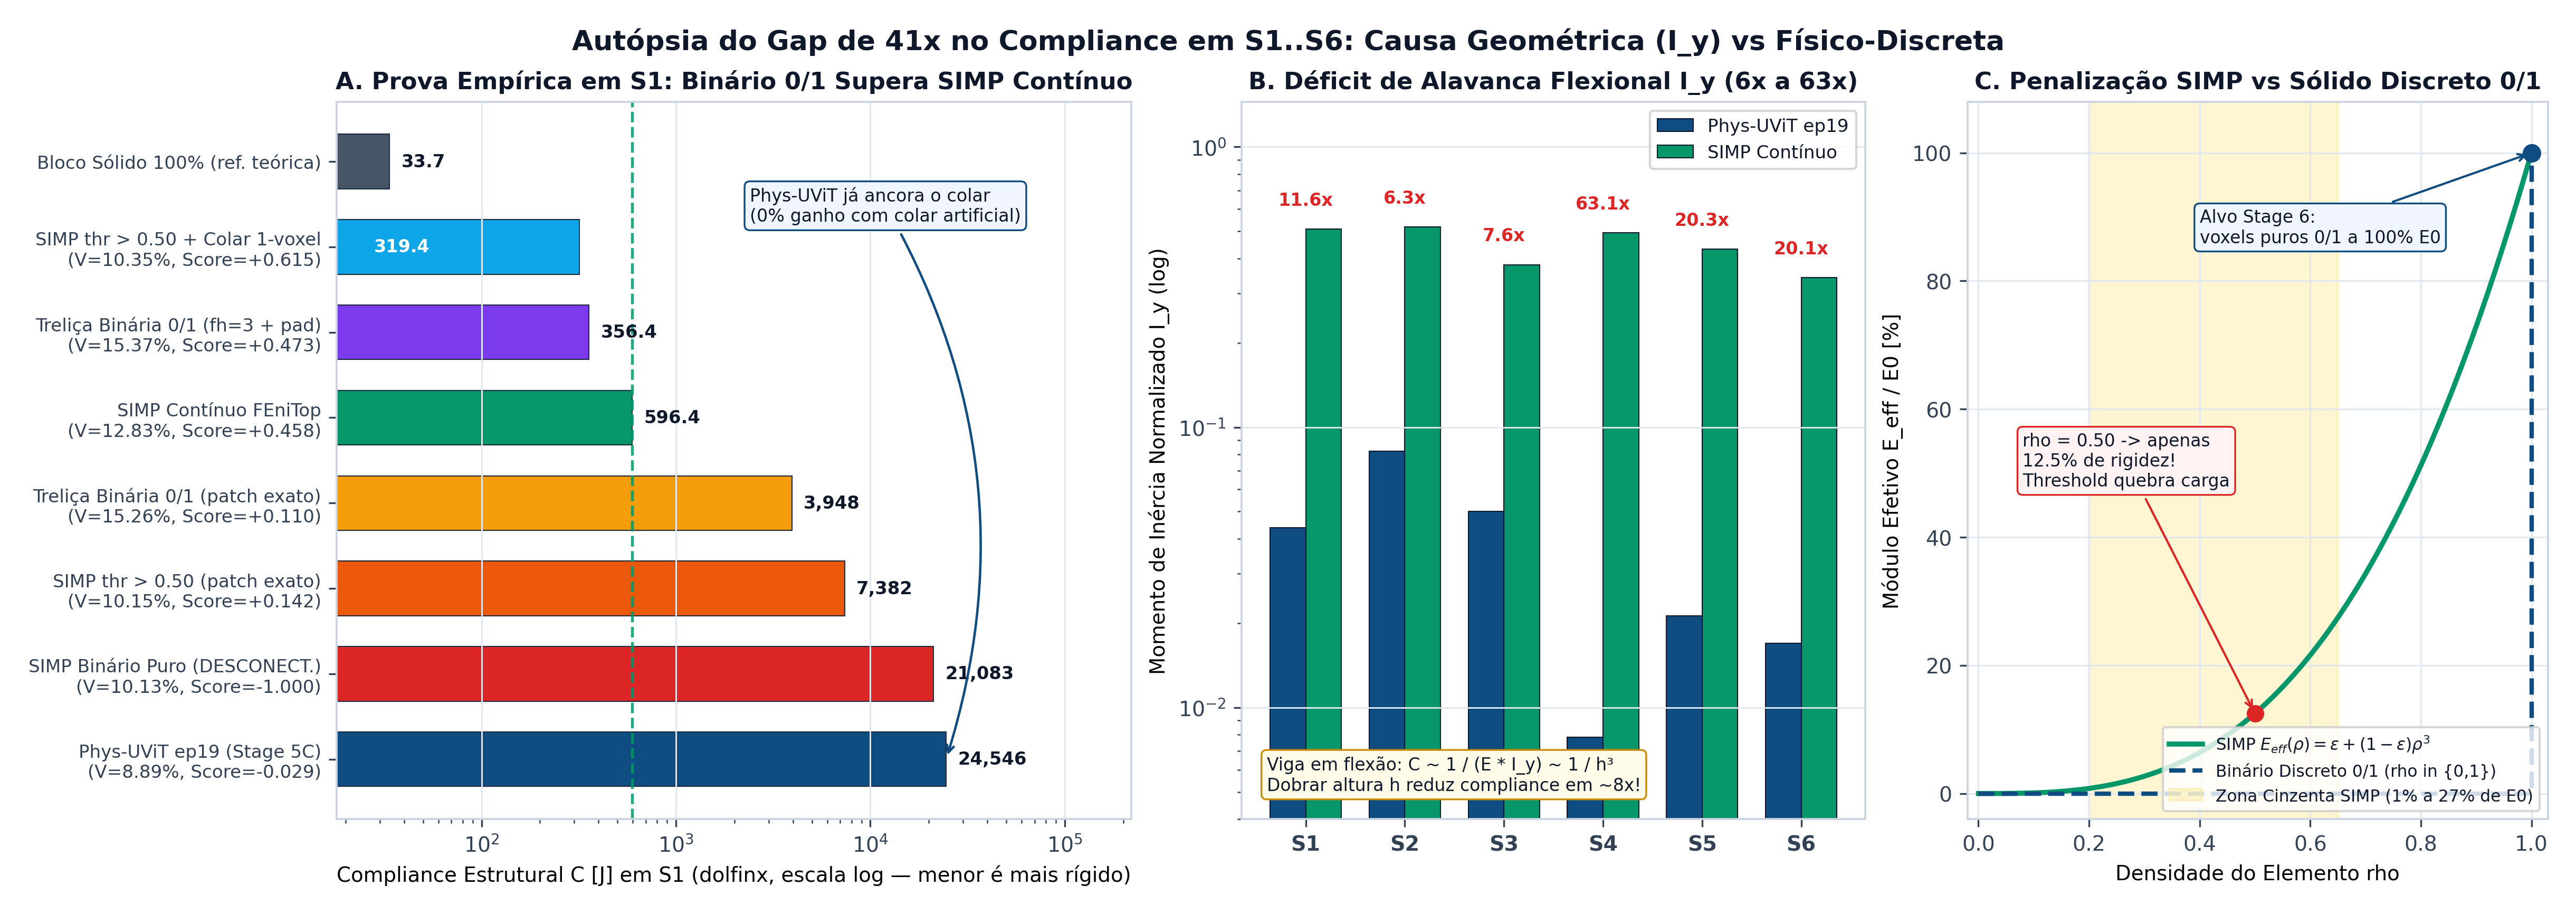
\includegraphics[width=\textwidth]{fig01_compliance_gap_autopsy.png}
\caption{Autópsia em \texttt{dolfinx} do gap de $41\times$ no compliance em \texttt{S1..S6}: prova de que estruturas binárias $0/1$ já superam o \texttt{SIMP contínuo} (A), déficit de inércia flexional $I_y$ entre $6.3\times$ e $63.1\times$ (B) e efeito $\rho^3$ na zona cinzenta (C).}
\label{fig:gap-autopsy}
\end{figure}

\section{Anatomia Numérica de \texttt{StructuredHex8FEM} (\texttt{fast\_amg}) vs. \texttt{DOLFINx}}

Para treinar via Self-Play em escala real, precisamos avaliar a resposta elástica e o mapa completo de $\mathrm{SED}_e$ em dezenas de milhares de topologias intermediárias. Invocar \texttt{DOLFINx} via compilação UFL em cada passo da Fase 2 consumia até $41.9\text{ s}$ em um único estado de \texttt{S6} — tempo incompatível com centenas de episódios por geração.

Para eliminar esse gargalo sem perder um dígito de exatidão física, implementamos em \texttt{alphabuilder/src/logic/selfplay/fast\_fem.py} o solver vetorizado \texttt{StructuredHex8FEM}:
\begin{enumerate}
\item \textbf{Montagem vetorizada em blocos $3\times 3$ (\texttt{BSR}):} cada nó interior conecta-se a $27$ blocos vizinhos no estêncil hexaédrico. Pré-computando o mapeamento fixo de $8$ lotes vetorizados (\texttt{\_asm\_slots}), montamos toda a matriz esparsa em \texttt{scipy.sparse.bsr\_matrix} sem nenhum laço em Python sobre os $16{,}384$ elementos.
\item \textbf{Multigrid Algébrico Suavizado (\texttt{PyAMG} v5.4.1) com Modos Rígidos:} passamos explicitamente os $6$ modos ortogonais de corpo rígido ($3$ translações e $3$ rotações em $\mathbb{R}^3$, \texttt{rbm\_modes}) para o pré-condicionador simétrico \texttt{smoothed\_aggregation\_solver} usando suavizador em blocos simétricos de Gauss--Seidel e fatoração LU esparsa exata \texttt{splu} no nível grosso (\texttt{max\_coarse=300}), acelerado por Gradiente Conjugado (\texttt{accel="cg"}).
\item \textbf{Projeção de modos nulos em apoios generalizados:} para lidar com pontes MBB bi-apoiadas, roletes $U_y$ ou engastes em dupla aba do Stage 6, o solver detecta automaticamente os eixos de translação global não fixados por \texttt{bc\_masks} e projeta a média desses eixos após o solve, impedindo deriva numérica do vetor $\mathbf{u}$.
\end{enumerate}

Durante os testes cruzados contra o \texttt{DOLFINx}, um bug instrutivo surgiu na primeira versão do extrator de energia de deformação em \texttt{evaluator.py}: usar \texttt{fem.Expression} no ponto central de cada elemento \texttt{DG0} sub-integrava os modos lineares de flexão do hexaedro trilinear (produzindo $329.86\text{ J}$ para $C = 346.42\text{ J}$). Ao substituir pela projeção exata de Galerkin sobre funções de teste constantes por elemento ($\int \boldsymbol{\sigma}(\mathbf{u}):\boldsymbol{\varepsilon}(\mathbf{u})\,\psi_e\,\mathrm{d}x$) em quadratura de grau $2$, ambos os códigos atingiram paridade de precisão de máquina (Tabela~\ref{tab:fem-parity}).

\begin{table}[htbp]
\centering
\caption{Paridade numérica verificada entre \texttt{fast\_amg} e \texttt{DOLFINx} com extração de \texttt{SED} ativada.}
\label{tab:fem-parity}
\resizebox{\textwidth}{!}{%
\begin{tabular}{@{}lcccc@{}}
\toprule
Conjunto de Teste & Erro Rel. Compliance $C$ & Erro Rel. $u_{\max}$ & Consistência $\sum \mathrm{SED}_e$ vs. $C$ & Latência Típica (\texttt{64x32x8}) \\
\midrule
Cenários Stage 5C (\texttt{S1..S6}, \texttt{FULL\_CLAMP} \& \texttt{RAIL\_XY}) & $1.11\times 10^{-10}$ a $1.25\times 10^{-6}$ & $\le 3.49\times 10^{-6}$ & $4.20\times 10^{-9}$ a $2.88\times 10^{-8}$ & $2.3$--$7.4\text{ s}$ (vs. $41.9\text{ s}$) \\
Generalização 3D (\texttt{DualPad+3D}, \texttt{MBB}, \texttt{DeepBeam}) & $4.50\times 10^{-11}$ a $1.05\times 10^{-7}$ & $3.10\times 10^{-8}$ a $2.54\times 10^{-7}$ & $< 10^{-5}$ (teste unitário) & $1.11$--$1.90\text{ s}$ \\
Malha \texttt{24x12x4} c/ cavidade (elemento a elemento) & $< 10^{-3}$ & $< 10^{-3}$ & $< 10^{-5}$ & $< 0.15\text{ s}$ \\
\bottomrule
\end{tabular}%
}
\end{table}

\chapter{O Paradigma AlphaBuilder: Otimização Estrutural como Jogo Sequencial}
\chaptermark{O Paradigma AlphaBuilder como Jogo Sequencial}

\section{Por Que Construir Passo a Passo Vence Abordagens \emph{One-Shot}}

Diante da fragilidade do \texttt{SIMP\_bin}, diversos trabalhos recentes empregaram GANs ou modelos de difusão para gerar topologias em um único passo \citep{nie2021topologygan,maze2023diffusion,behzadi2021realtime,nobari2024towards,nobari2025optimize}. Contudo, geradores diretos padecem de ausência de restrição topológica forte: em domínios novos ou cargas excêntricas, falhas de um único voxel rompem a transmissão da carga ao apoio e invalidam toda a peça \citep{behzadi2023taming,huang2022closer}.

Inspirado pela síntese de busca em árvore e redes neurais profundas \citep{silver2016mastering,silver2017mastering,gaymann2019deep,luo2022alphatruss,garayalde2025mastering}, o \textbf{AlphaBuilder} formula o projeto estrutural diretamente sobre o conjunto discreto $\{0, 1\}^N$ como um \textbf{Processo de Decisão de Markov (MDP) em duas fases} (Figura~\ref{fig:mdp-tikz}).

\begin{figure}[htbp]
\centering
\begin{tikzpicture}[
  node distance=1.8cm and 2.1cm,
  state/.style={rectangle,rounded corners=4pt,draw=abNavy,fill=abBgBlue,thick,minimum height=1.15cm,align=center,font=\small\bfseries,inner sep=6pt},
  phase/.style={rectangle,rounded corners=4pt,draw=abEmerald,fill=abBgGreen,thick,minimum height=1.15cm,align=center,font=\small\bfseries,inner sep=6pt},
  term/.style={rectangle,rounded corners=4pt,draw=abViolet,fill=abViolet!10!white,thick,minimum height=1.15cm,align=center,font=\small\bfseries,inner sep=6pt},
  arr/.style={-{Stealth[length=2.5mm]},thick,abSlate}
]
\node[state] (s0) {Estado Vazio\\$V = 0\%$ (Fase 1)};
\node[state,right=of s0] (p1) {MCTS \texttt{GROWTH}\\Lotes \texttt{ADD} 6-conexos\\PBRS $\Phi(s)$};
\node[phase,right=of p1] (p2) {MCTS \texttt{REFINEMENT}\\Oráculo \texttt{fast\_amg}\\Lotes $16 \to 8$ (\texttt{ADD/REM})};
\node[term,below=1.1cm of p2] (end) {Terminal Real $R_{\mathrm{FEM}}$\\Backprop + \texttt{SED} + \texttt{fem\_probes}};

\draw[arr] (s0) -- (p1);
\draw[arr] (p1) edge[loop above] node[above,font=\scriptsize]{Desconectado} (p1);
\draw[arr] (p1) -- node[above,font=\scriptsize]{$P(\mathrm{conn})=1$} (p2);
\draw[arr] (p2) edge[loop above] node[above,font=\scriptsize]{$t \le N_{\max}$} (p2);
\draw[arr] (p2) -- node[right,font=\scriptsize]{Fim / Colapso $-1$} (end);
\end{tikzpicture}
\caption{Máquina de estados finitos do jogo construtivo AlphaBuilder: transição causal da Fase 1 (\texttt{GROWTH}) sem física elástica para a Fase 2 (\texttt{REFINEMENT}) sob supervisão completa do oráculo FEM.}
\label{fig:mdp-tikz}
\end{figure}

Na \textbf{Fase 1 (\texttt{GROWTH})}, a peça nasce do zero ($\boldsymbol{\rho} = \mathbf{0}$). As jogadas legais (\texttt{get\_legal\_add\_moves}) limitam o acréscimo de material aos vizinhos de face (\emph{6-conectividade}) da massa existente e da vizinhança imediata dos apoios, sempre bloqueados onde \texttt{domain\_mask = 0}. Para cruzar vãos longos em poucos turnos, cada passo executa micro-lotes de \texttt{32} adições (\texttt{action\_batch\_size=32}). Assim que uma única ilha sólida une o engaste a toda a zona carregada (\texttt{check\_structure\_connectivity}), ocorre a transição para a \textbf{Fase 2 (\texttt{REFINEMENT})}. Nela, qualquer remoção sobre células de suporte ou carregamento é rigorosamente proibida (\texttt{get\_protected\_regions}), o problema elástico torna-se bem-posto e o agente esculpe aberturas e reforços consultando o oráculo FEM real.

\section{PBRS Generalizado com Decaimento Linear em Fase 1}

Enquanto a estrutura está desconectada em Fase 1, $\mathbf{K}(\boldsymbol{\rho})$ é singular — logo, nenhum gradiente elástico existe. Para evitar vagar cego em domínios nunca vistos sem corromper o ótimo final da Fase 2, adotamos \textbf{Potential-Based Reward Shaping (PBRS)} com decaimento linear em gerações \citep{wang2020warmstart,muller2025improving}. O potencial escalar generalizado em \texttt{reward.py} mede:
\begin{equation}
\Phi(s) = w_{\mathrm{conn}}\, f_{\mathrm{conn}}(s)
+ w_{\mathrm{dist}}\max\!\left(0,\; 1 - \frac{d_{\min}(s)}{D_{\mathrm{diag}}}\right)\mathbb{I}[f_{\mathrm{conn}}(s) < 0.999]
- P_{\mathrm{island}}(s),
\end{equation}
com $w_{\mathrm{conn}} = 0.50$, $w_{\mathrm{dist}} = 0.25$, diagonal normalizadora $D_{\mathrm{diag}} = \sqrt{D^2+H^2+W^2}$ e menor distância euclidiana $d_{\min}(s)$ entre a superfície conectada ao apoio e os voxels de carga faltantes. Na avaliação foliar do MCTS, o valor heurístico mistura-se à predição neural via peso linearmente decrescente $\alpha(g)$:
\begin{equation}
V_{\mathrm{leaf}}(s) = \big(1 - \alpha(g)\big)\,V_{\mathrm{net}}(s) + \alpha(g)\,\Phi(s), \qquad
\alpha(g) = 0.30\,\max\!\left(0,\; 1 - \frac{g}{5}\right).
\end{equation}
Duas garantias decorrem imediatamente dessa forma: no instante em que $f_{\mathrm{conn}} = 1$, o termo de aproximação espacial anula-se identicamente, não atraindo massa inútil depois da conexão; e na geração $5$, $\alpha(5) = 0$, devolvendo $100\%$ da decisão à rede neural calibrada.

\section{Recompensa \texttt{v3.3}, Lei de Alavancagem e Mecânica de Euler--Bernoulli}

Uma vez conectada a estrutura, sua qualidade física objetiva é governada exclusivamente pelas equações calibradas de \texttt{reward.py}:
\begin{align}
S_C(C) &= \operatorname{clip}\!\big(1.15 - 0.35\,(\log_{10}(\max(C, 1)) - 1),\; -0.60,\; 0.90\big), \\
B_V(V) &= \operatorname{clip}\!\big(2.5\,(0.10 - V),\; -0.60,\; 0.30\big), \\
R(C, V, u_{\max}) &= \operatorname{clip}\!\big(S_C(C) + B_V(V),\; -1.0,\; 1.0\big) - P_{u_{\max}},
\end{align}
onde a penalidade de pré-colapso $P_{u_{\max}}$ permanece nula até $70\%$ do limite físico (\texttt{DISPLACEMENT\_LIMIT\_RAW = 128,000}), cresce linearmente até $-0.50$ ao atingir $128{,}000$ e termina o episódio em $-1.0$ acima desse teto ou na desconexão.

\begin{eurekabox}{A Lei de Alavancagem $10^{7.143\,\Delta V}$ e o Efeito $49\times$ de Euler--Bernoulli}
Calculando a razão entre as derivadas parciais na região linear da recompensa \texttt{v3.3}:
\begin{equation}
\left|\frac{\partial R / \partial V}{\partial R / \partial \log_{10} C}\right| = \frac{2.5}{0.35} \approx 7.143
\quad\Longrightarrow\quad
\frac{C_{\mathrm{antes}}}{C_{\mathrm{depois}}}\Bigg|_{\Delta R = 0} = 10^{7.143\,\Delta V}.
\end{equation}
Investir $\Delta V = +4\%$ de massa extra custa apenas $-0.100$ de Score — lucro garantido sempre que a compliance cair acima de $1.93\times$. Ainda mais decisivo: pela teoria de Euler--Bernoulli ($C \propto \frac{F^2 L^3}{3 E I_y}$), para uma \textbf{mesma quantidade fixa de massa} ($V=10\%$, isto é, $\Delta V = 0$!), separar $4$ voxels centrais em dois banzos de espessura $2$ nas bordas superior e inferior ($H_{\mathrm{ext}}=32$, $h_{\mathrm{int}}=28$) altera o momento de inércia de $I_y^{\mathrm{rasa}} = 4^3/12 = 5.33$ para $I_y^{\mathrm{vazada}} = (32^3 - 28^3)/12 = 901.33$ — um salto teórico de $169\times$ na inércia pura (e $\sim 49\times$ mesmo descontando flexibilidade por cisalhamento na alma)! Logo, a recompensa \texttt{v3.3} \emph{nunca} impediu estruturas rígidas: a rede pré-Self-Play estava apenas cega ao ganho de alavanca $I_y$.
\end{eurekabox}

\begin{figure}[htbp]
\centering
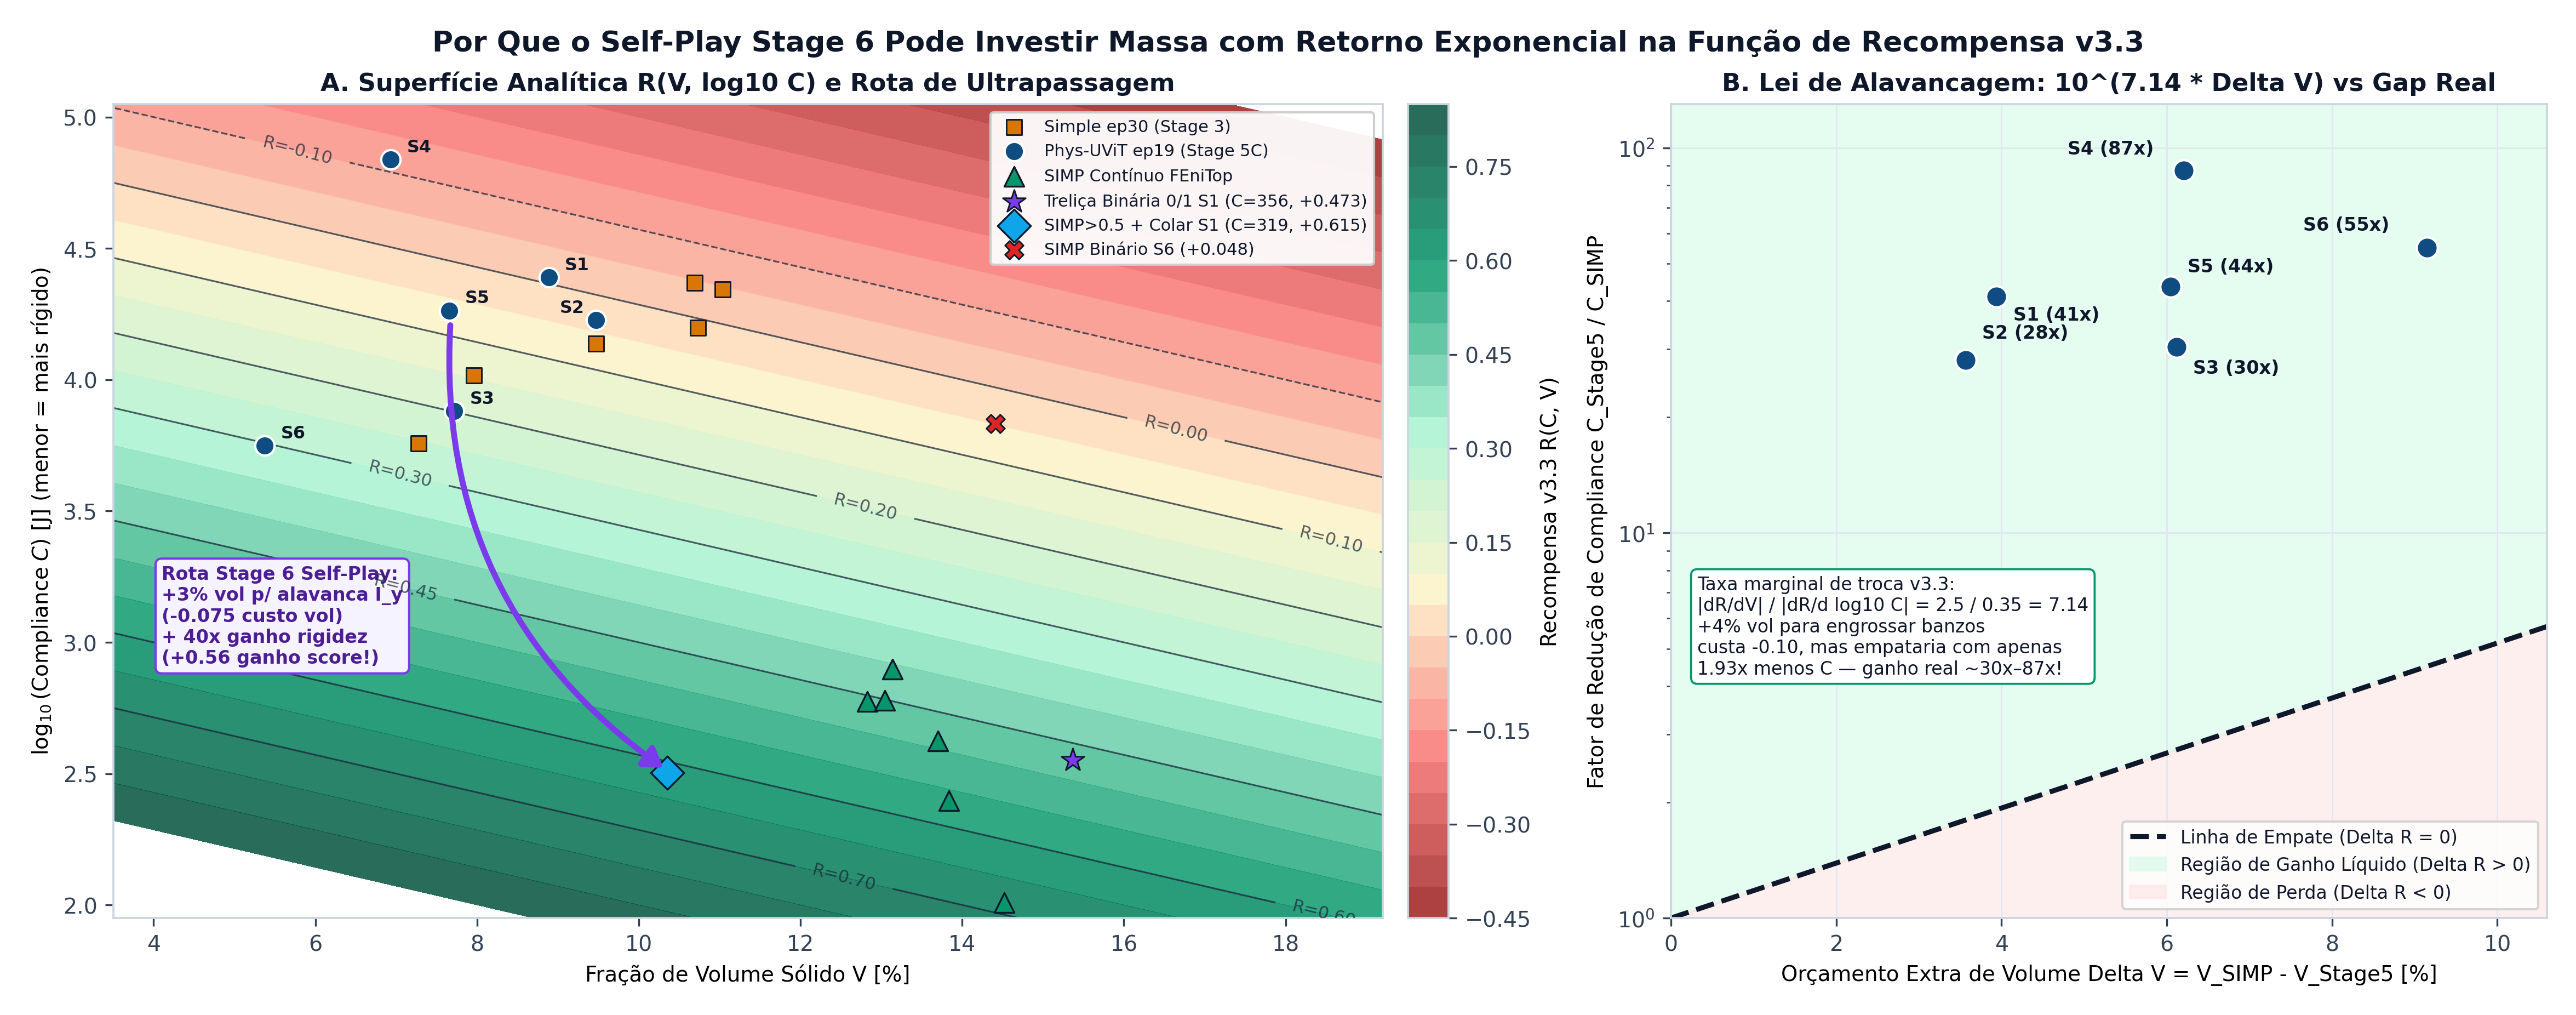
\includegraphics[width=\textwidth]{fig02_reward_landscape_and_overtaking_path.png}
\caption{Superfície exata de recompensa \texttt{v3.3} $R(V, \log_{10} C)$ com testemunhas empíricas em \texttt{dolfinx} e rota analítica de ultrapassagem do Stage 6 (A), acompanhada da lei de empate $10^{7.14\Delta V}$ frente ao ganho real disponível nos cenários \texttt{S1..S6} (B).}
\label{fig:reward-landscape}
\end{figure}

\section{Mecânica Profunda do MCTS: \emph{Virtual Loss}, \emph{MixMax} e Retropropagação}

Para escalar avaliações neurais em mini-lotes (\texttt{batch\_size = 8}) dentro da árvore \citep{kocsis2006bandit,browne2012survey,rosin2011multi}, o motor \texttt{AlphaBuilderMCTS} usa \emph{Virtual Loss} \citep{wu2019accelerating} combinado ao operador \textbf{MixMax} do \emph{AlphaTruss} \citep{luo2022alphatruss}:
\begin{equation}
a^* = \arg\max_{a \in \mathcal{A}_{\mathrm{top}\text{-}k}(s)} \left[ Q_{\mathrm{mix}}(s, a) + c_{\mathrm{puct}}\, P(s, a)\, \frac{\sqrt{\sum_b N(s, b)}}{1 + N(s, a) + n_{\mathrm{vl}}(s, a)} \right],
\end{equation}
onde $Q_{\mathrm{mix}}(s,a) = \beta \frac{W(s,a)}{N(s,a)} + (1-\beta)\max_{\tau} V(\tau)$ com $\beta = 0.75$ na Fase 1 (impedindo que caminhos fracassados afoguem o único ramo que encontrou a carga) e $\beta = 1.0$ na Fase 2 (preservando esperança estatística imparcial). Após a poda de \texttt{top\_k = 64} candidatos em \texttt{MCTSNode.expand}, os priors mantidos são renormalizados estritamente para $\sum_a P(s,a) = 1.0$. Ao término do episódio, \texttt{backpropagate\_value\_targets} atribui alvos de valor assimétricos às duas fases no SQLite: em Fase 1 aplica-se retorno descontado até o passo da conexão $t_{\mathrm{P2}}$ ($v_t = \gamma^{t_{\mathrm{P2}}-t} R_{\mathrm{final}}$, $\gamma = 0.99$), enquanto em Fase 2 interpola-se a recompensa real do oráculo FEM ($v_t = (1-\lambda_t) R_{\mathrm{FEM}}(t) + \lambda_t R_{\mathrm{final}}$), preservando $-1.0$ para desconexões e colapsos.

\chapter{O Dataset de Warmup, Simetrias Físicas e o Teto da Imitação}

\section{Coleta de Warmup (\texttt{Data Harvest}) e Armazenamento Compacto}

Para não iniciar o aprendizado de RL por tentativa aleatória cega em $16{,}384$ voxels, o projeto gerou o banco de treinamento supervisionado \texttt{v3.3} (\texttt{warmup\_v3\_3\_kaggle.db} + \texttt{split\_v3\_3.json} disjunto por cenário) a partir de duas rotinas em \texttt{alphabuilder/src/logic/harvest/}:
\begin{itemize}
\item \textbf{\texttt{BEZIER}:} sintetiza pontes contínuas suaves entre engastes e cargas aleatórias por curvas de Bézier quadráticas, registrando quadros de crescimento conectivo (Fase 1) e aplicando \texttt{FEniTop} para produzir trajetórias de refinamento em Fase 2.
\item \textbf{\texttt{FULL\_DOMAIN}:} otimiza todo o domínio contínuo via \texttt{FEniTop}, fornecendo alvos globais auxiliares (\texttt{v\_constructed\_blob} para a \texttt{blueprint\_head}) e medições reais de $R_{\mathrm{FEM}}$ e $\log_{10} C$.
\end{itemize}
Os tensores de política esparsa são serializados no formato binário \texttt{COO1} e matrizes densas em \texttt{.npy} comprimido com \emph{zlib}, carregados em bloco contíguo na RAM com baixa sobrecarga sob múltiplos workers (\texttt{TopologyDatasetV31}).

\section{\emph{Negative Sampling} Reformulado e Leis Exatas de Escala}

Se um modelo aprender valor apenas em estados quase ótimos do SIMP, ele superestimará estruturas defeituosas no jogo real. Em \texttt{alphabuilder/src/neural/augmentation.py}, aplicamos quatro aumentos físicos ativos:
\begin{enumerate}
\item \textbf{\texttt{erosion\_attack}} sobre estados finais para calibrar sensibilidade à perda de seção.
\item \textbf{\texttt{sabotage}} e \textbf{\texttt{saboteur}} sobre estados de Fase 2, removendo regiões ativas e desabilitando alvos de compliance (\texttt{comp\_valid = False}, \texttt{conn\_valid = False}) quando a conectividade é corrompida.
\item \textbf{\texttt{load\_multiplier} ($k = 3.0$):} escala o campo vetorial $\mathbf{f} \leftarrow 3\,\mathbf{f}$ sem tocar nos voxels sólidos! Pela linearidade exata de $\mathbf{K}\mathbf{u}=\mathbf{f}$, $\mathbf{u}$ triplica e a compliance cresce com o quadrado do fator ($k^2 = 9$):
\begin{equation}
C(3\mathbf{F}) = 9\,C(\mathbf{F}) \quad\Longrightarrow\quad \log_{10} C(3\mathbf{F}) = \log_{10} C(\mathbf{F}) + 2\log_{10} 3 \approx \log_{10} C(\mathbf{F}) + 0.9542.
\end{equation}
Ao mesmo tempo, \texttt{bp\_valid} é desmarcado porque a geometria ótima para $3\times$ carga exigiria outro volume ótimo.
\end{enumerate}

\section{Equivariância Exata sob o Grupo \texorpdfstring{$D_4 \times \mathbb{Z}_2$}{D4 x Z2} (\texttt{16x})}

Como a elasticidade linear isotrópica é invariante a isometrias ortogonais $\mathbf{Q} \in O(3)$ do espaço, toda rotação ou reflexão que preserve os alinhamentos da malha regular hexaédrica constitui uma simetria física exata sem perda de informação. No domínio padrão $(64, 32, 8)$ — e igualmente nas resoluções múltiplas de $4$ do Tier 3 — exploramos o grupo diedral completo \textbf{$D_4 \times \mathbb{Z}_2$ de ordem $16$}:
\begin{itemize}
\item Em \texttt{\_\_getitem\_\_}, sorteiam-se $2^3 = 8$ combinações de reflexões independentes (\texttt{flip\_x}, \texttt{flip\_y}, \texttt{flip\_z}), invertendo estritamente o sinal da componente de força correspondente ($f_x \leftarrow -f_x$ sob \texttt{flip\_x}, etc.) enquanto mantém escalares ($\rho$, \texttt{blueprint}, \texttt{domain\_mask}, \texttt{sed\_target}) positivos.
\item No agrupador por lote (\texttt{make\_symmetry\_collate\_fn}), aplica-se com probabilidade $50\%$ uma rotação de $90^\circ$ em $Z$ (\texttt{torch.rot90(..., dims=(2,3))}), mapeando $(64,32,8) \leftrightarrow (32,64,8)$ com $0\%$ de \emph{padding} e transformando vetores e condições de contorno segundo a álgebra exata de planos ortogonais:
\begin{equation}
(f_x',\, f_y') = (-f_y,\, f_x), \qquad (m_x',\, m_y') = (m_y,\, m_x).
\end{equation}
\end{itemize}

\section{O Problema do \emph{Covariate Shift} (Desvio de Covariáveis)}

Mesmo equipado com $16\times$ simetrias e regularização de carga, o treinamento puramente supervisionado sobre trajetórias geradas pelo \texttt{SIMP} enfrenta uma barreira clássica: o \textbf{desvio de covariáveis (\emph{Covariate Shift})}. Na validação, a rede avalia estados pertencentes ao mesmo fluxo suave de otimização que gerou o dataset ($V \approx 13\%$, $I_y \approx 0.45$--$0.52$). Na inferência autônoma a partir do zero, pequenas escolhas iniciais da Fase 1 conduzem o estado por geometrias intermediárias inéditas (barras finas, ângulos abruptos, ausência de zona cinzenta). Como essas distribuições nunca entraram nos dados de treino, a rede sofre um salto abrupto de erro apenas fora de sua distribuição original — exatamente o fenômeno que verificaremos no Capítulo 5.

\chapter{Da U-Net Local à \texttt{Phys-UViT 3D}: Engenharia Arquitetural Baseada em Física}
\chaptermark{Da U-Net Local à Phys-UViT 3D}

\section{Crítica Estrutural aos Predecessores (\texttt{Simple} e \texttt{Swin-UNETR})}

A definição da arquitetura definitiva em \texttt{alphabuilder/src/neural/phys\_uvit.py} emergiu diretamente das restrições físicas do domínio $64 \times 32 \times 8$ em contraste com redes convencionais de visão 3D \citep{dosovitskiy2021image,liu2021swin,hatamizadeh2022swin,vaswani2017attention}:

\begin{itemize}
\item O modelo convolucional \textbf{\texttt{Simple}} ($1.66\text{M}$ params, Figura~\ref{fig:arch-simple}) depende de campos receptivos locais construídos por blocos \texttt{Conv3d}. Nos vãos alongados, os passos iniciais próximos à parede $x=0$ não acoplam suficientemente a geometria exata da carga distal, resultando em $4.43\%$ de material excedente além do ponto carregado (\emph{overshoot} em $X$) e em falhas topológicas de múltiplas ilhas.
\item O \textbf{\texttt{Swin-UNETR}} do MONAI impõe divisibilidade por $32$ devido aos seus $4$ estágios de redução e janelas locais $7\times 7\times 7$ (Figura~\ref{fig:arch-swin}). Como o domínio tem espessura $Z = 8$, preencher $8 \to 32$ introduz \textbf{$+300\%$ de \emph{zero-padding} morto}, desperdiçando memória e cálculo sobre voxels vazios artificiais e introduzindo artefatos de fronteira ao recortar o retorno.
\end{itemize}

\begin{figure}[htbp]
\centering
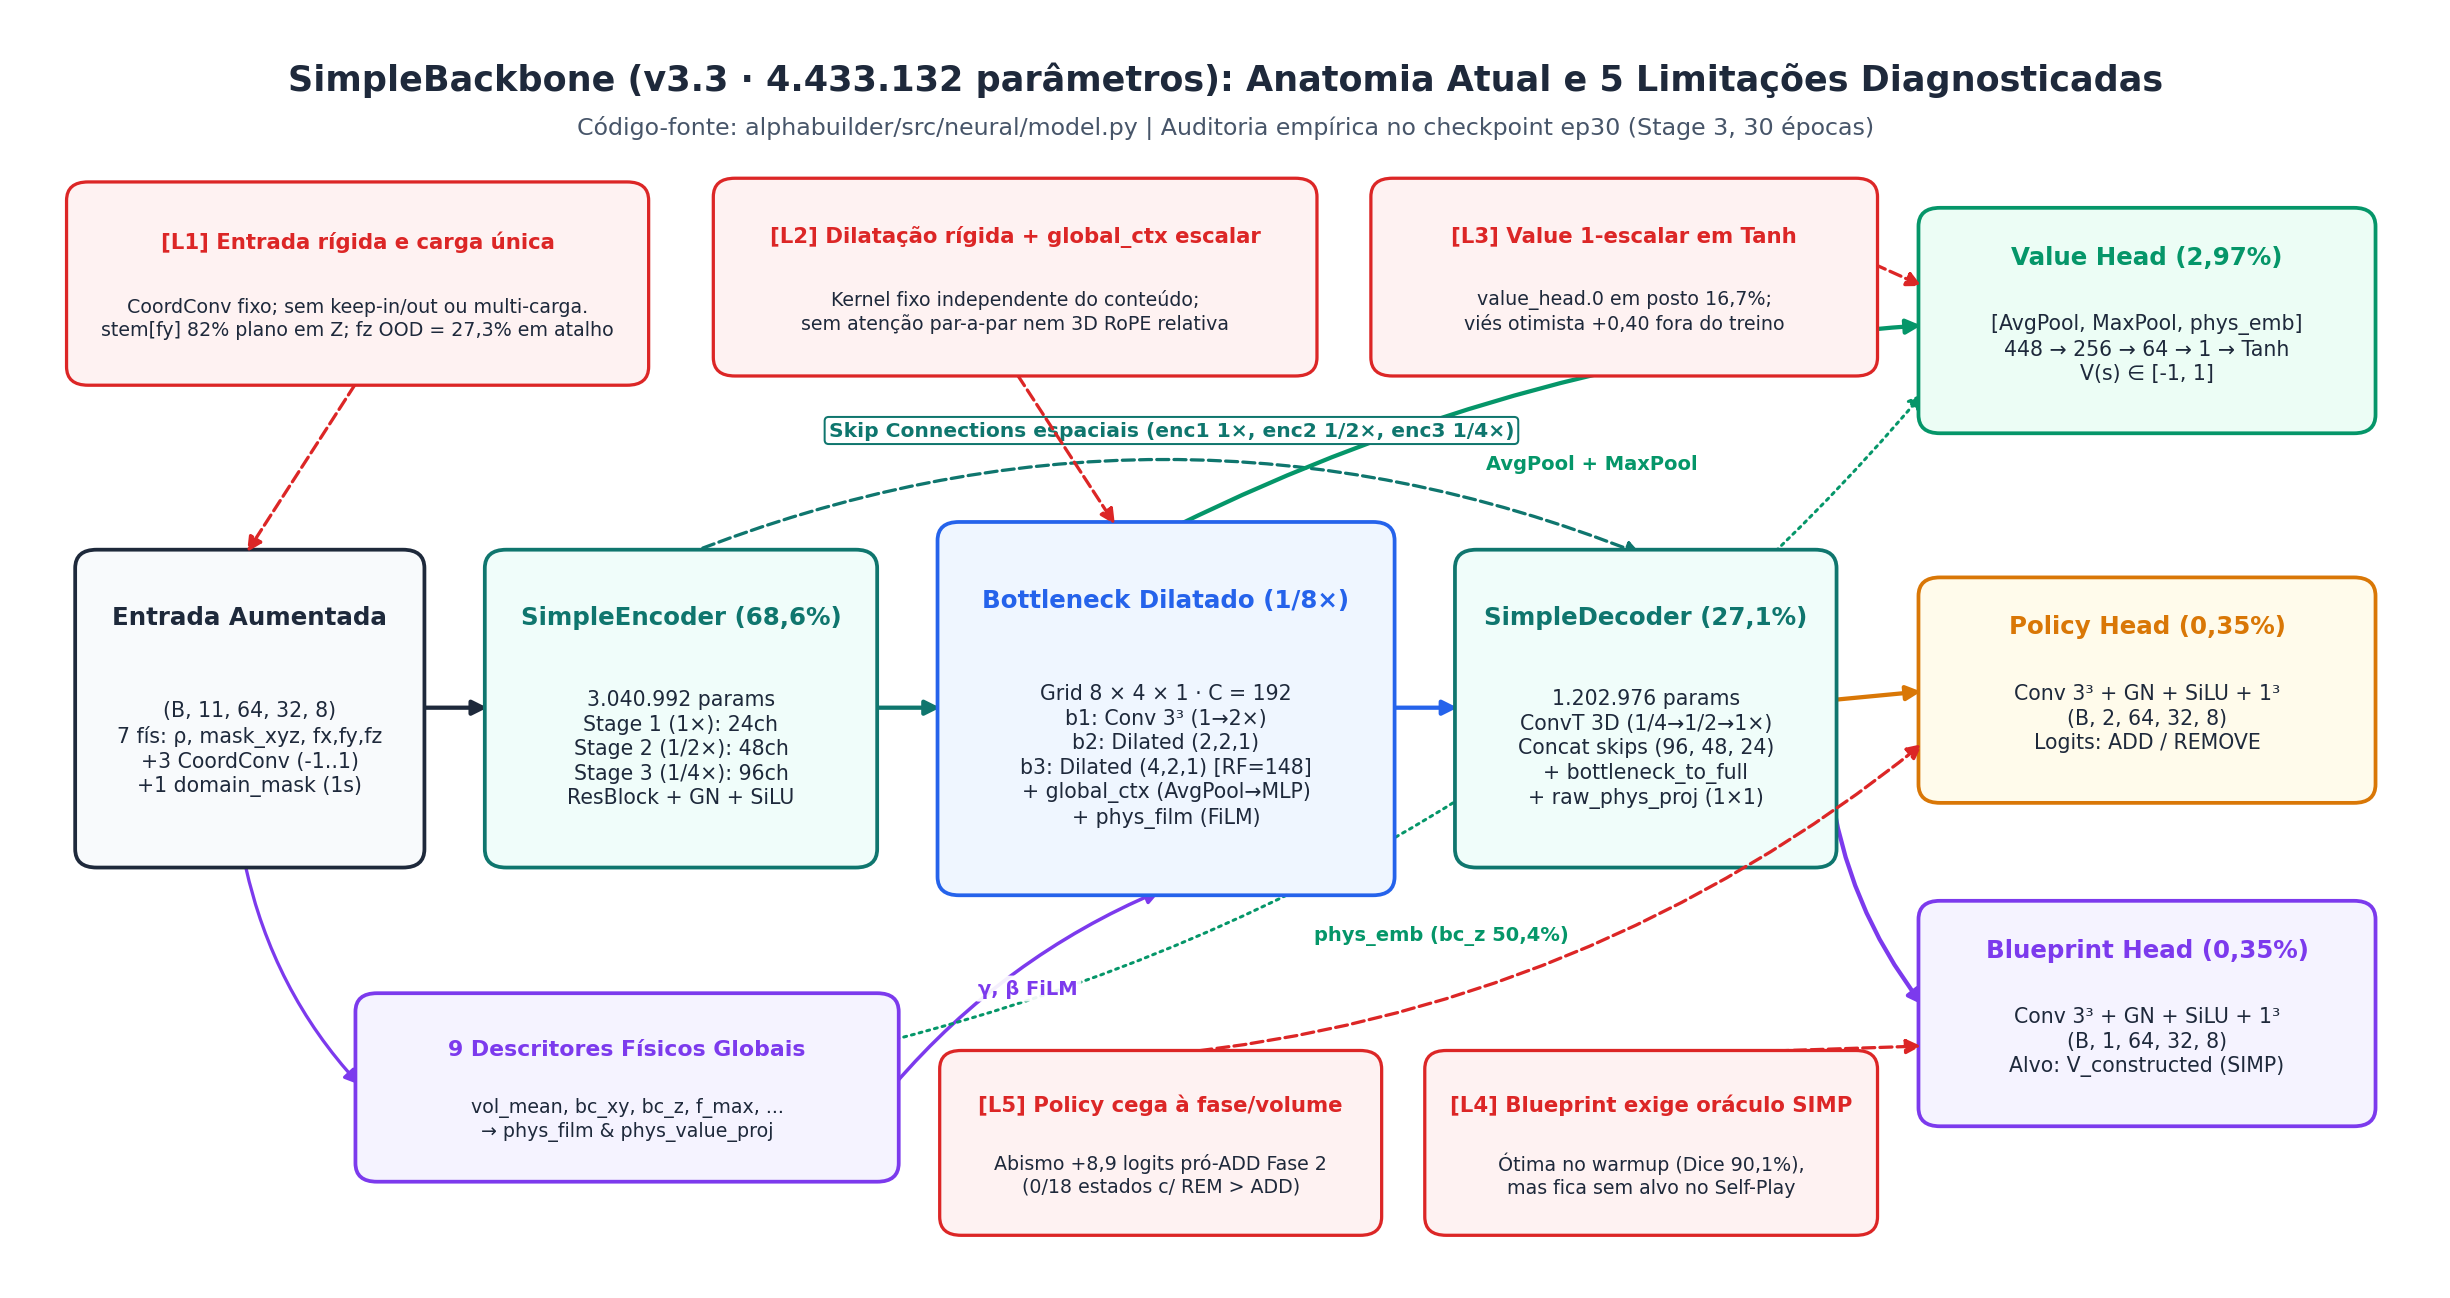
\includegraphics[width=\textwidth]{arch_01_simple_backbone_anatomy.png}
\caption{Anatomia do baseline convolucional \texttt{Simple} (\texttt{1.66M} params) evidenciando dependência de campo receptivo local e gargalo estreito.}
\label{fig:arch-simple}
\end{figure}

\begin{figure}[htbp]
\centering
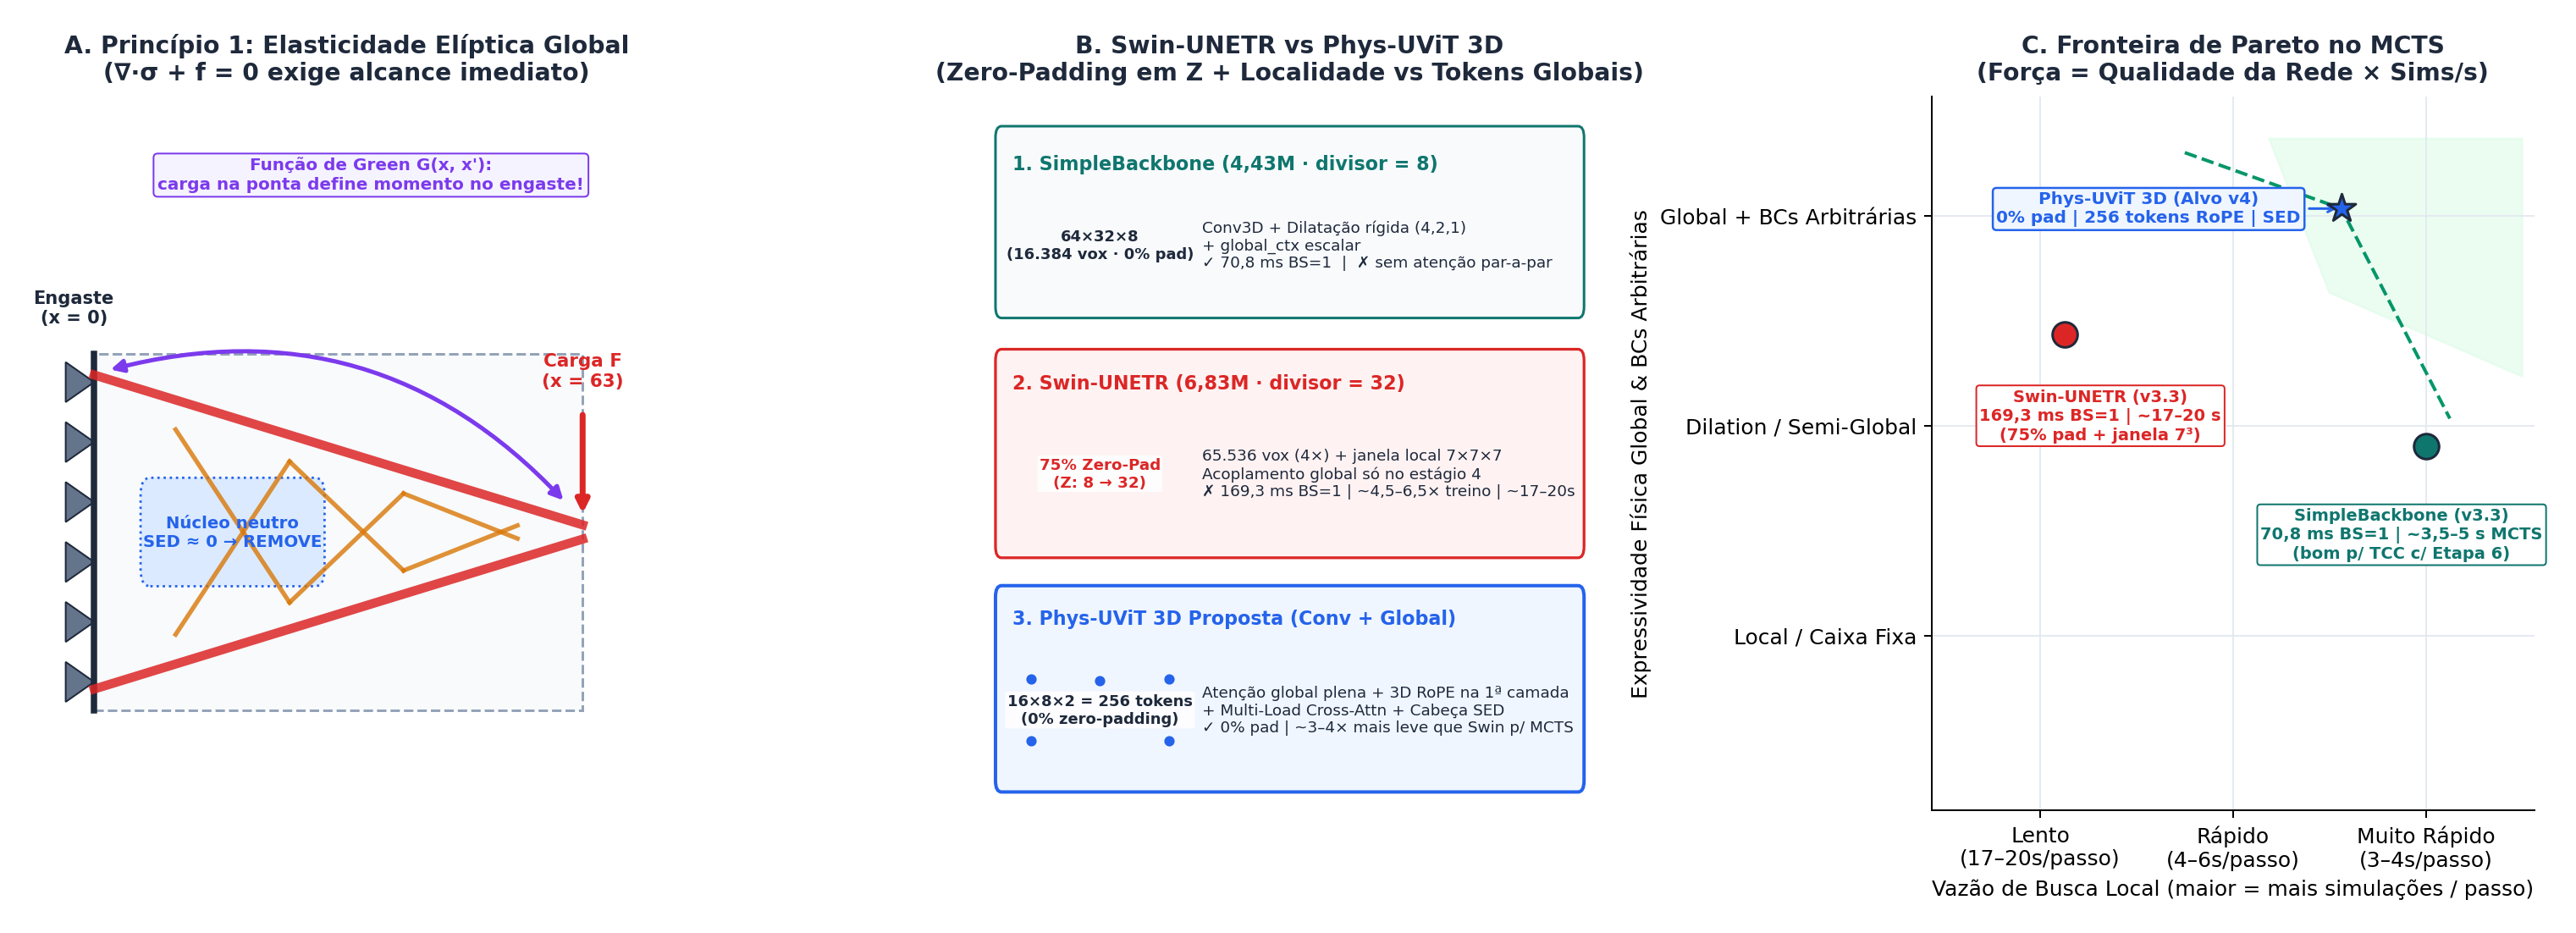
\includegraphics[width=\textwidth]{arch_02_first_principles_vs_swin.png}
\caption{Derivação a partir de primeiros princípios geométricos: por que o requisito \texttt{divisor=32} do \texttt{Swin-UNETR} inflava o volume em $+300\%$ no eixo $Z$ frente ao \texttt{divisor=4}.}
\label{fig:arch-swin}
\end{figure}

\section{Anatomia Completa da \texttt{Phys-UViT 3D} (\texorpdfstring{$4{,}912{,}683$}{4,912,683} Parâmetros)}

Desenhada para resolver simultaneamente alcance global instantâneo, invariância de resolução e fatoração física, a \texttt{Phys-UViT 3D} (Figuras~\ref{fig:macro-arch}, \ref{fig:internal-mech} e \ref{fig:uvit-3d}) apoia-se em cinco pilares:

\begin{enumerate}
\item \textbf{\texttt{divisor=4} nativo ($0\%$ \emph{padding}):} duas reduções espaciais por $2\times$ levam $64\times 32\times 8$ exatamente a $16\times 8\times 2 = \mathbf{256\text{ tokens}}$, consumindo apenas $4.942\text{ GB}$ de VRAM em pico e treinando a $227.1\text{ amostras/s}$ em $2\times\text{T4}$.
\item \textbf{Atenção Global e \texttt{3D RoPE} Relativo:} cinco blocos \texttt{GlobalPhysicsTransformerBlock} ($\text{embed\_dim}=192$, $6$ cabeças, \emph{SwiGLU} + \texttt{AdaLN(phys)}) acoplam todo o engaste a toda a carga em complexidade quadrática modesta $O(256^2) = 65{,}536$ pares por camada. Empregando \emph{Rotary Position Embeddings} 3D relativos $(\Delta x, \Delta y, \Delta z)$ em vez de tabelas absolutas fixas, a arquitetura generaliza nativamente para malhas \texttt{Tier 3} como $48\times 24\times 12$ e $64\times 24\times 8$.
\item \textbf{\texttt{MultiLoadEncoder3D} e \texttt{domain\_mask}:} codifica múltiplas cargas vetoriais independentemente de sua ordem e mascara regiões proibidas (\emph{keep-out}) via \texttt{domain\_mask}, normalizando estatísticas físicas invariantes a $D_4\times\mathbb{Z}_2$ dentro do volume útil $V_{\mathrm{eff}}$.
\item \textbf{Cabeça Fatorada \texttt{FactoredValueHead}:} separa probabilidade de conectividade $p_{\mathrm{conn}} = \sigma(z_{\mathrm{conn}})$ e predição logarítmica de compliance $\hat{\ell}_C = \widehat{\log_{10} C}$, compondo analiticamente o valor segundo a fórmula exata de recompensa \texttt{v3.3} acrescida de um resíduo pequeno $\delta_{\mathrm{res}}(s)$:
\begin{equation}
\hat{V}(s) = \sigma(z_{\mathrm{conn}})\,\Big[\operatorname{clip}\big(S_C(10^{\hat{\ell}_C}) + B_V(V_{\mathrm{eff}}),\; -1.0,\; 1.0\big)\Big]
+ \big(1 - \sigma(z_{\mathrm{conn}})\big)(-1.0) + \delta_{\mathrm{res}}(s).
\end{equation}
\item \textbf{Cabeça Densa \texttt{sed\_head}:} saída volumétrica dedicada $(B, 4, D, H, W)$ cujo primeiro canal prevê $\log(1+\mathrm{SED}_e)$ em cada voxel (inativa no Stage 5 com $4{,}884{,}839$ pesos treinados e ativada no Stage 6 com $4{,}912{,}683$ parâmetros).
\end{enumerate}

\begin{figure}[htbp]
\centering
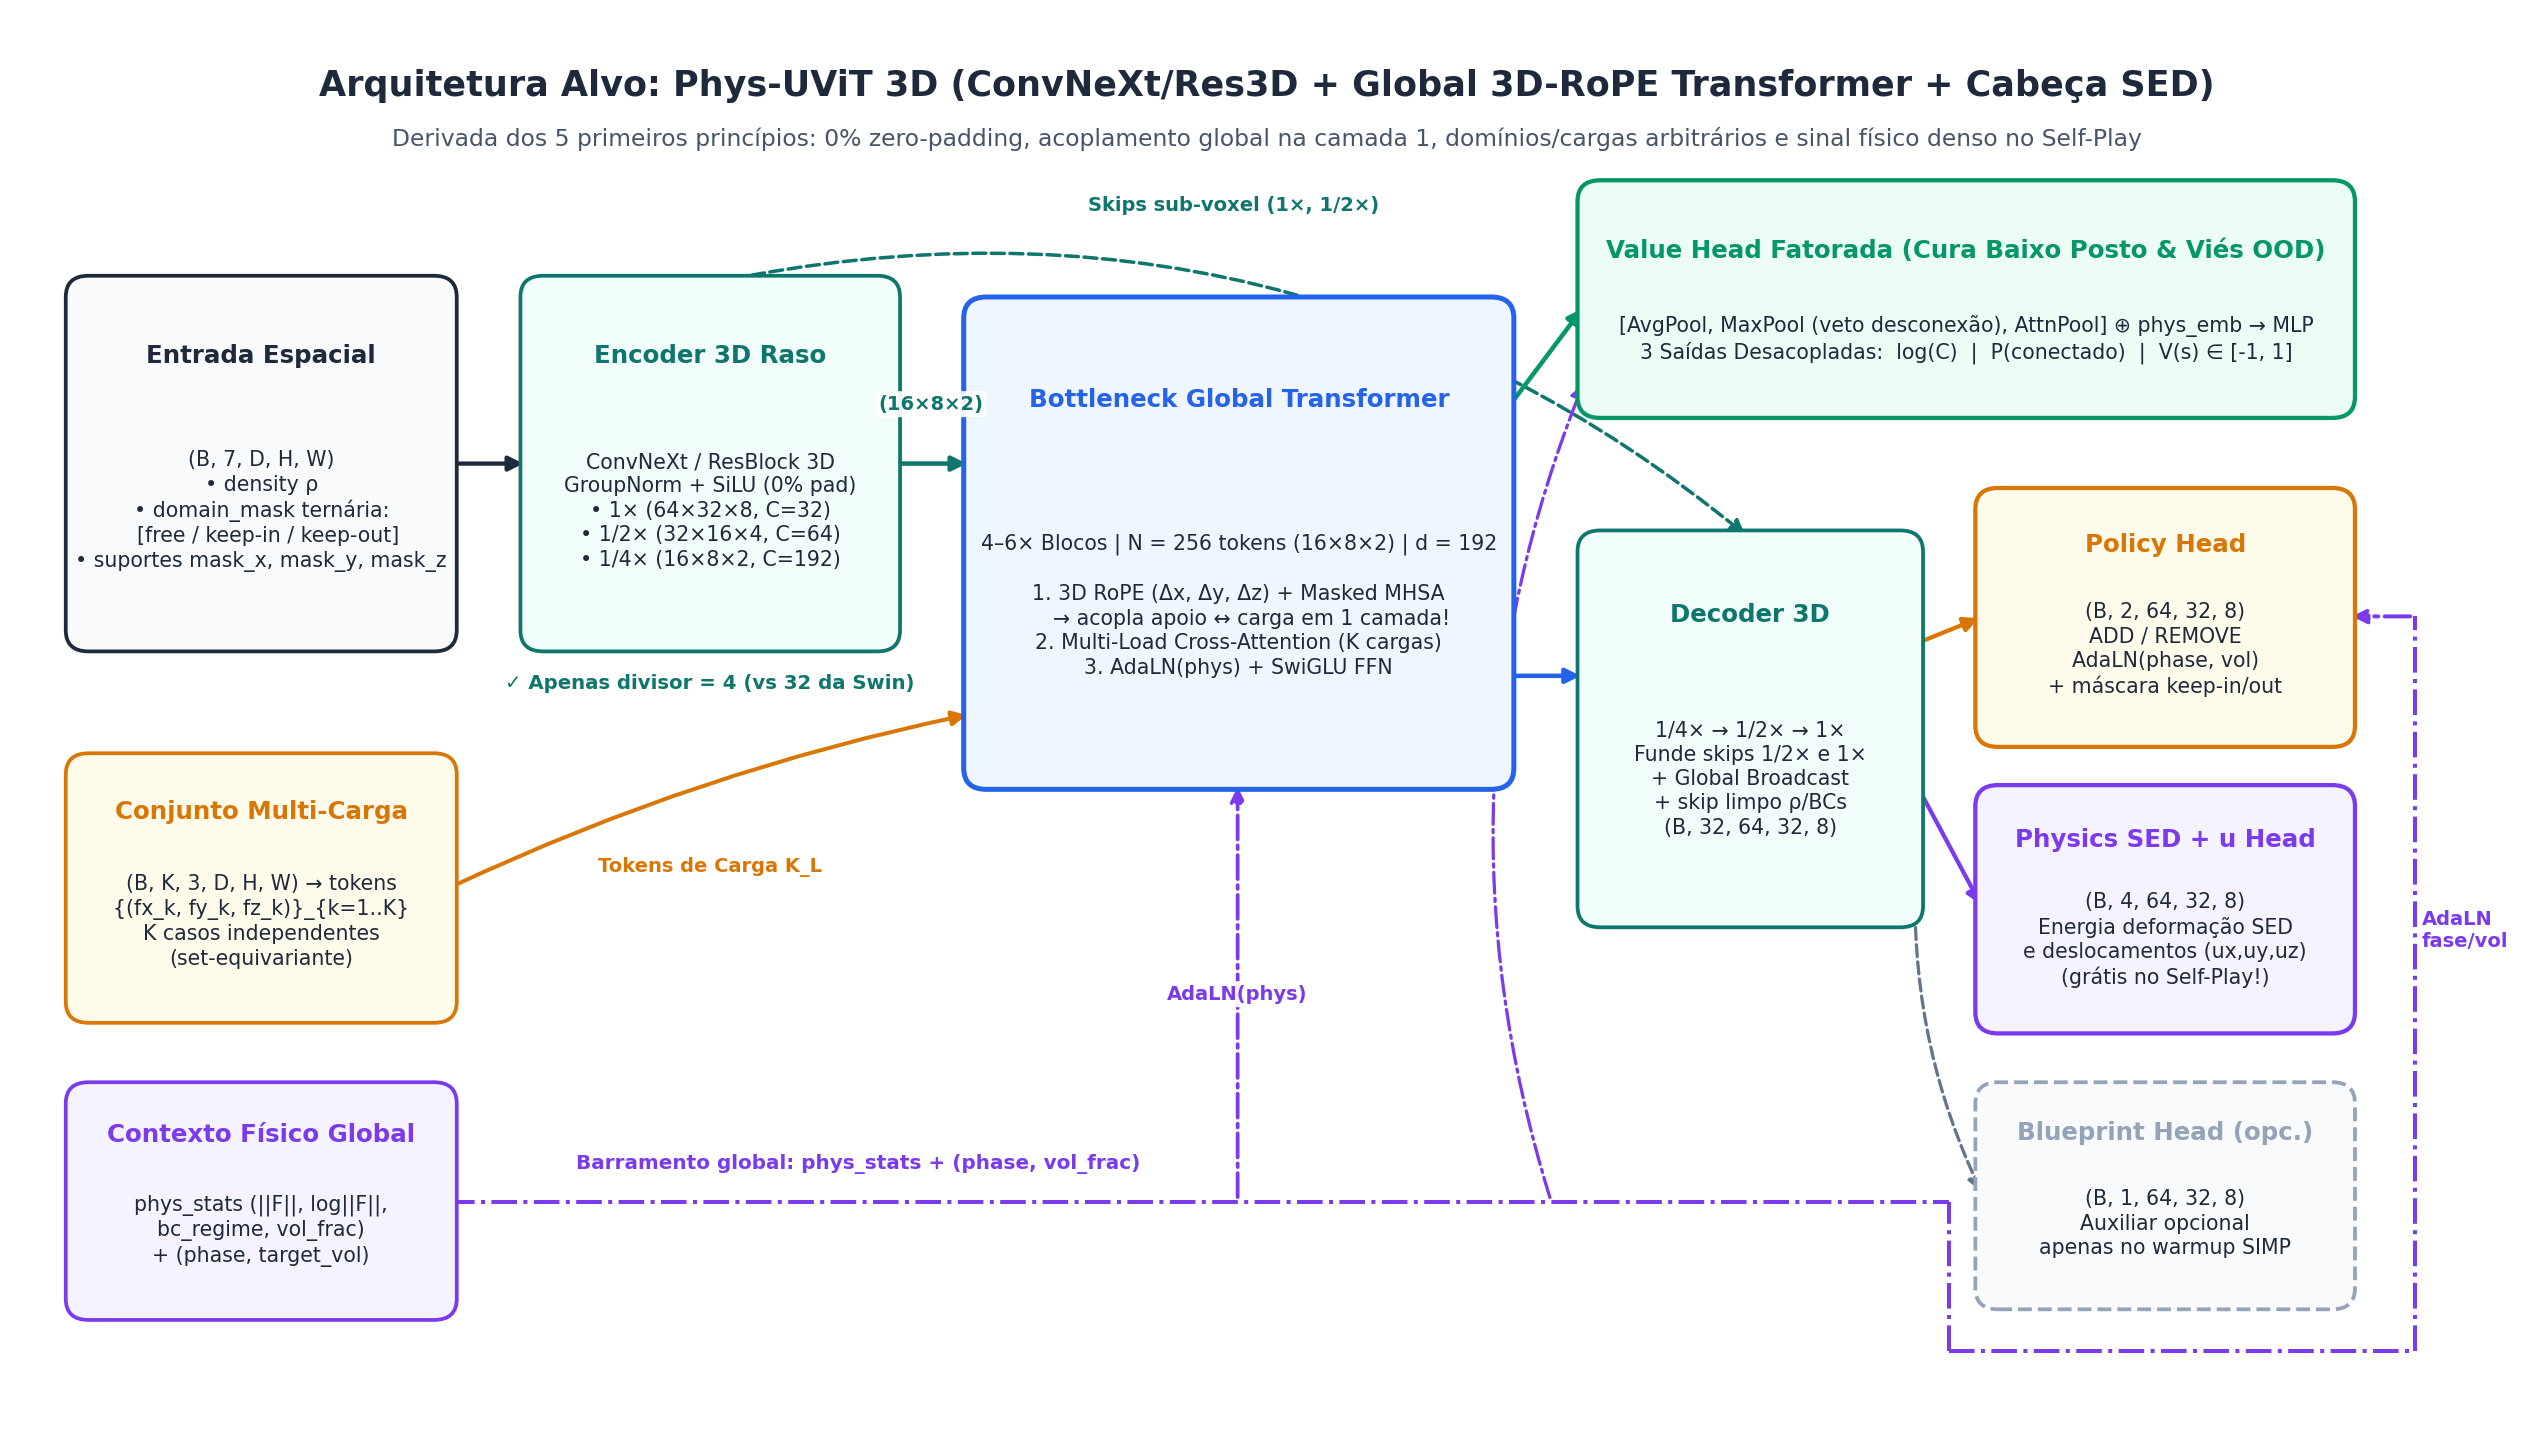
\includegraphics[width=\textwidth]{arch_03_macro_architecture.png}
\caption{Macro-arquitetura \texttt{Phys-UViT 3D}: encoder raso \texttt{divisor=4}, gargalo Transformer global de 256 tokens e cabeças físicas desacopladas.}
\label{fig:macro-arch}
\end{figure}

\begin{figure}[htbp]
\centering
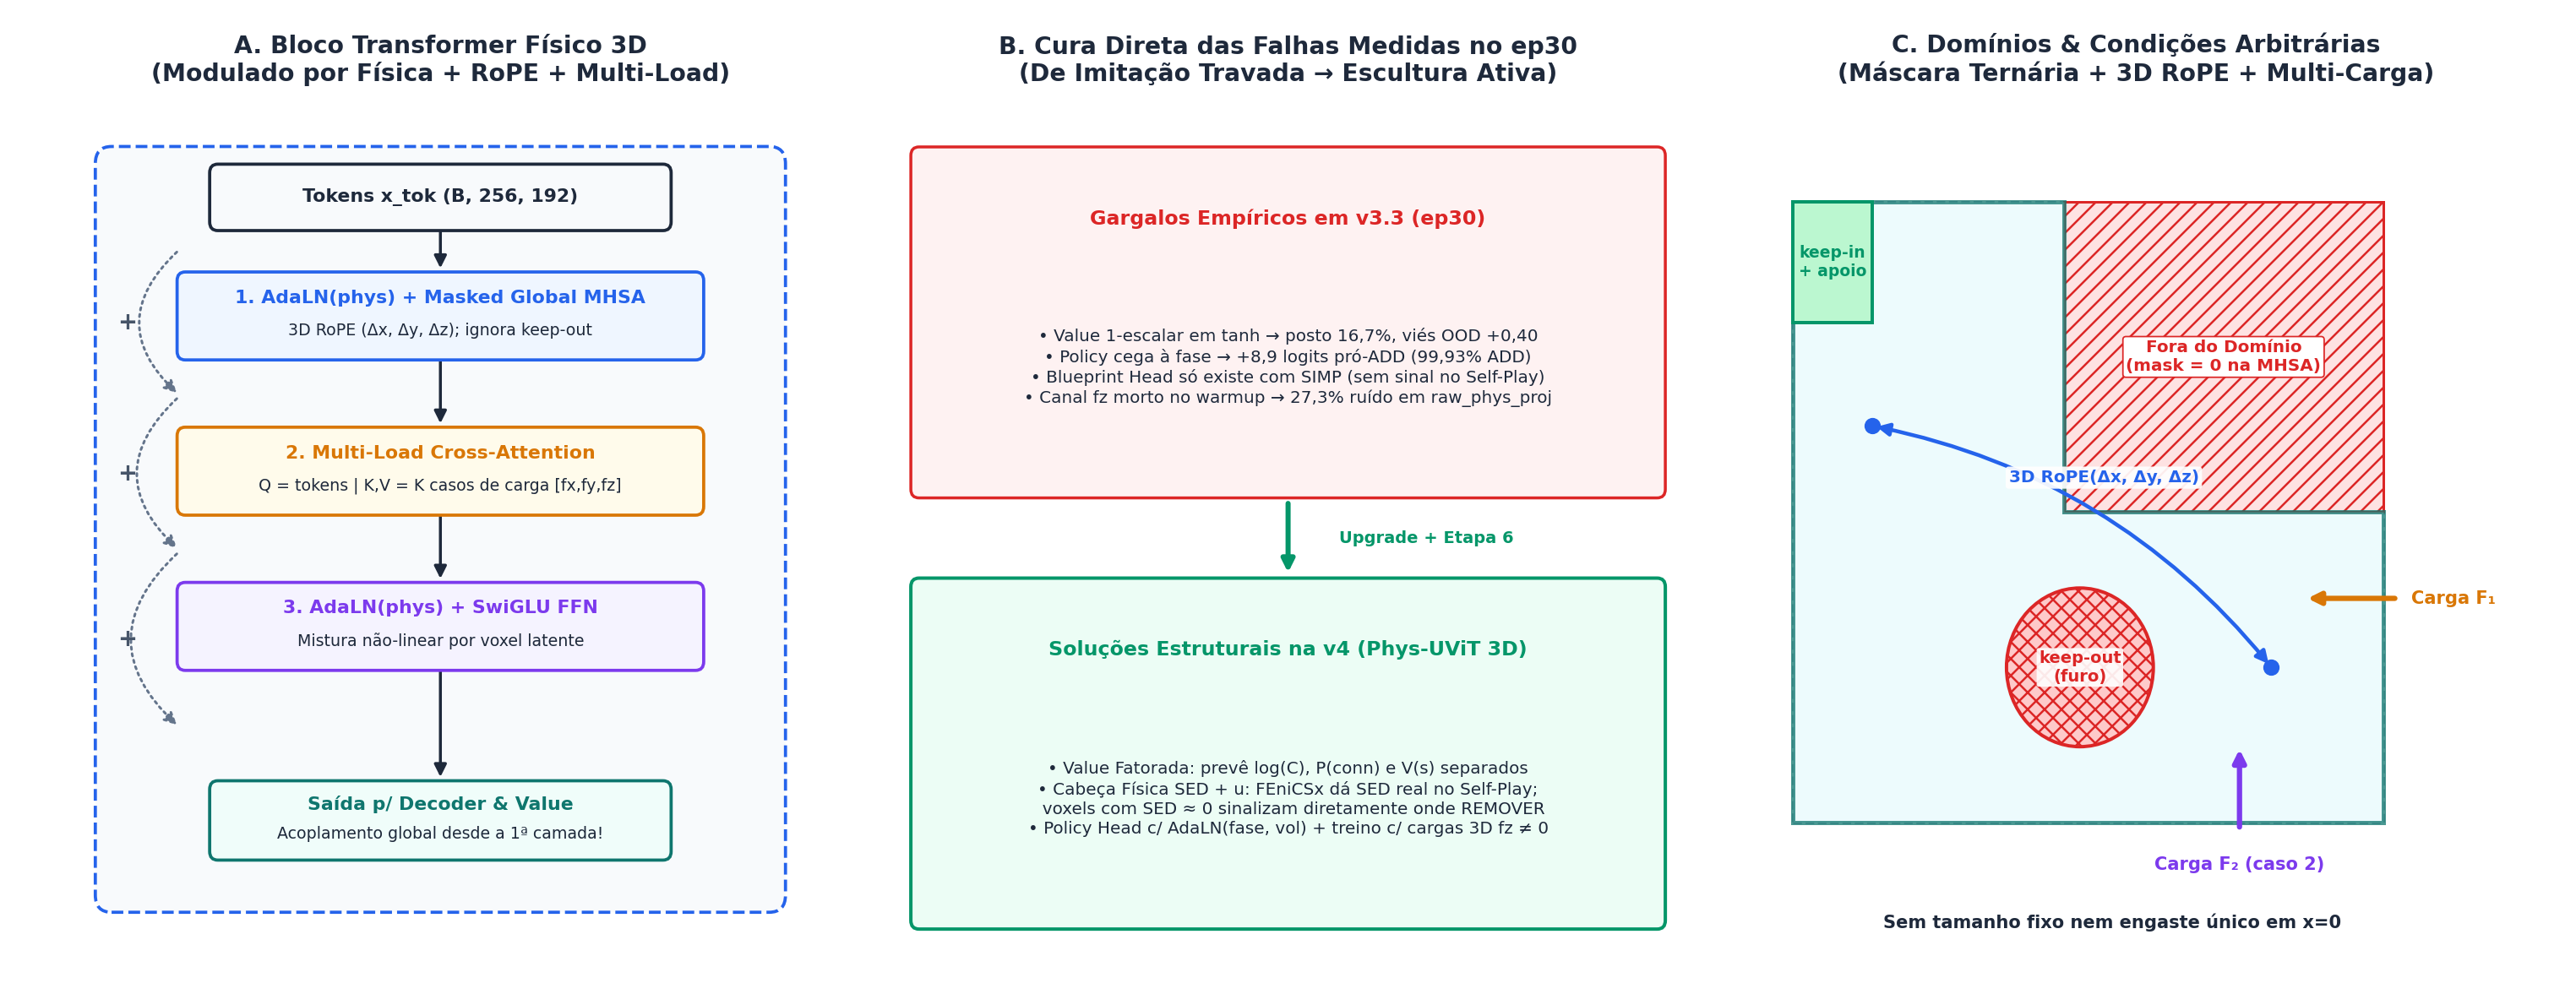
\includegraphics[width=\textwidth]{arch_04_internal_mechanisms.png}
\caption{Mecanismos internos da \texttt{Phys-UViT 3D}: codificação de múltiplas cargas, rotação relativa \texttt{3D RoPE} e simetria $D_4\times\mathbb{Z}_2$.}
\label{fig:internal-mech}
\end{figure}

\begin{figure}[htbp]
\centering
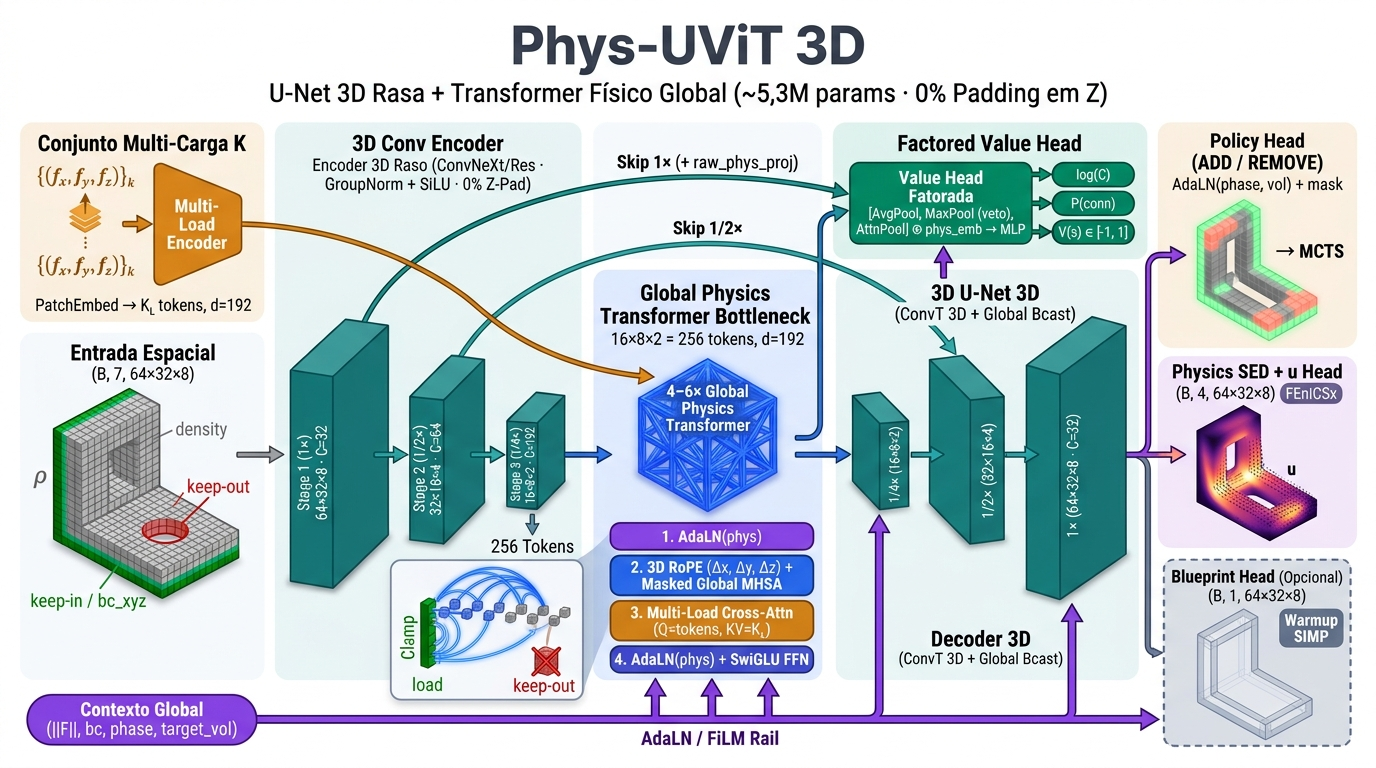
\includegraphics[width=\textwidth]{arch_06_phys_uvit_3d_illustration.png}
\caption{Visualização tridimensional esquemática do fluxo de tensores na \texttt{Phys-UViT 3D} conectando apoios distantes às regiões carregadas.}
\label{fig:uvit-3d}
\end{figure}

\section{Dinâmica Real de Treinamento (Stage 3 vs. Stage 5) e GPU vs. TPU}

Ao longo de $30$ épocas no Kaggle $2\times\text{Tesla T4}$ ($15.75\text{h}$ de relógio / $31.50\text{ GPU-h}$), a \texttt{Phys-UViT 3D} atingiu seu ponto ótimo na \textbf{Época 19}, superando o baseline \texttt{Simple ep30} em todas as métricas principais de validação (Figuras~\ref{fig:train-dyn}, \ref{fig:val-heads} e \ref{fig:losses-comp}): \texttt{Val Total Loss = 0.3285}, \texttt{Val Core = 0.3272} ($-4.2\%$ frente a $0.3415$), \texttt{Value MAE = 0.0117} (pico $0.0111$ vs. $0.0134$), \texttt{Blueprint Dice = 90.81\%} (pico $91.02\%$), \texttt{log10(C) MAE = 0.0352} décadas (pico $0.0319$) e \texttt{Conn Acc = 99.998\%} (pico $100.0\%$).

\begin{figure}[htbp]
\centering
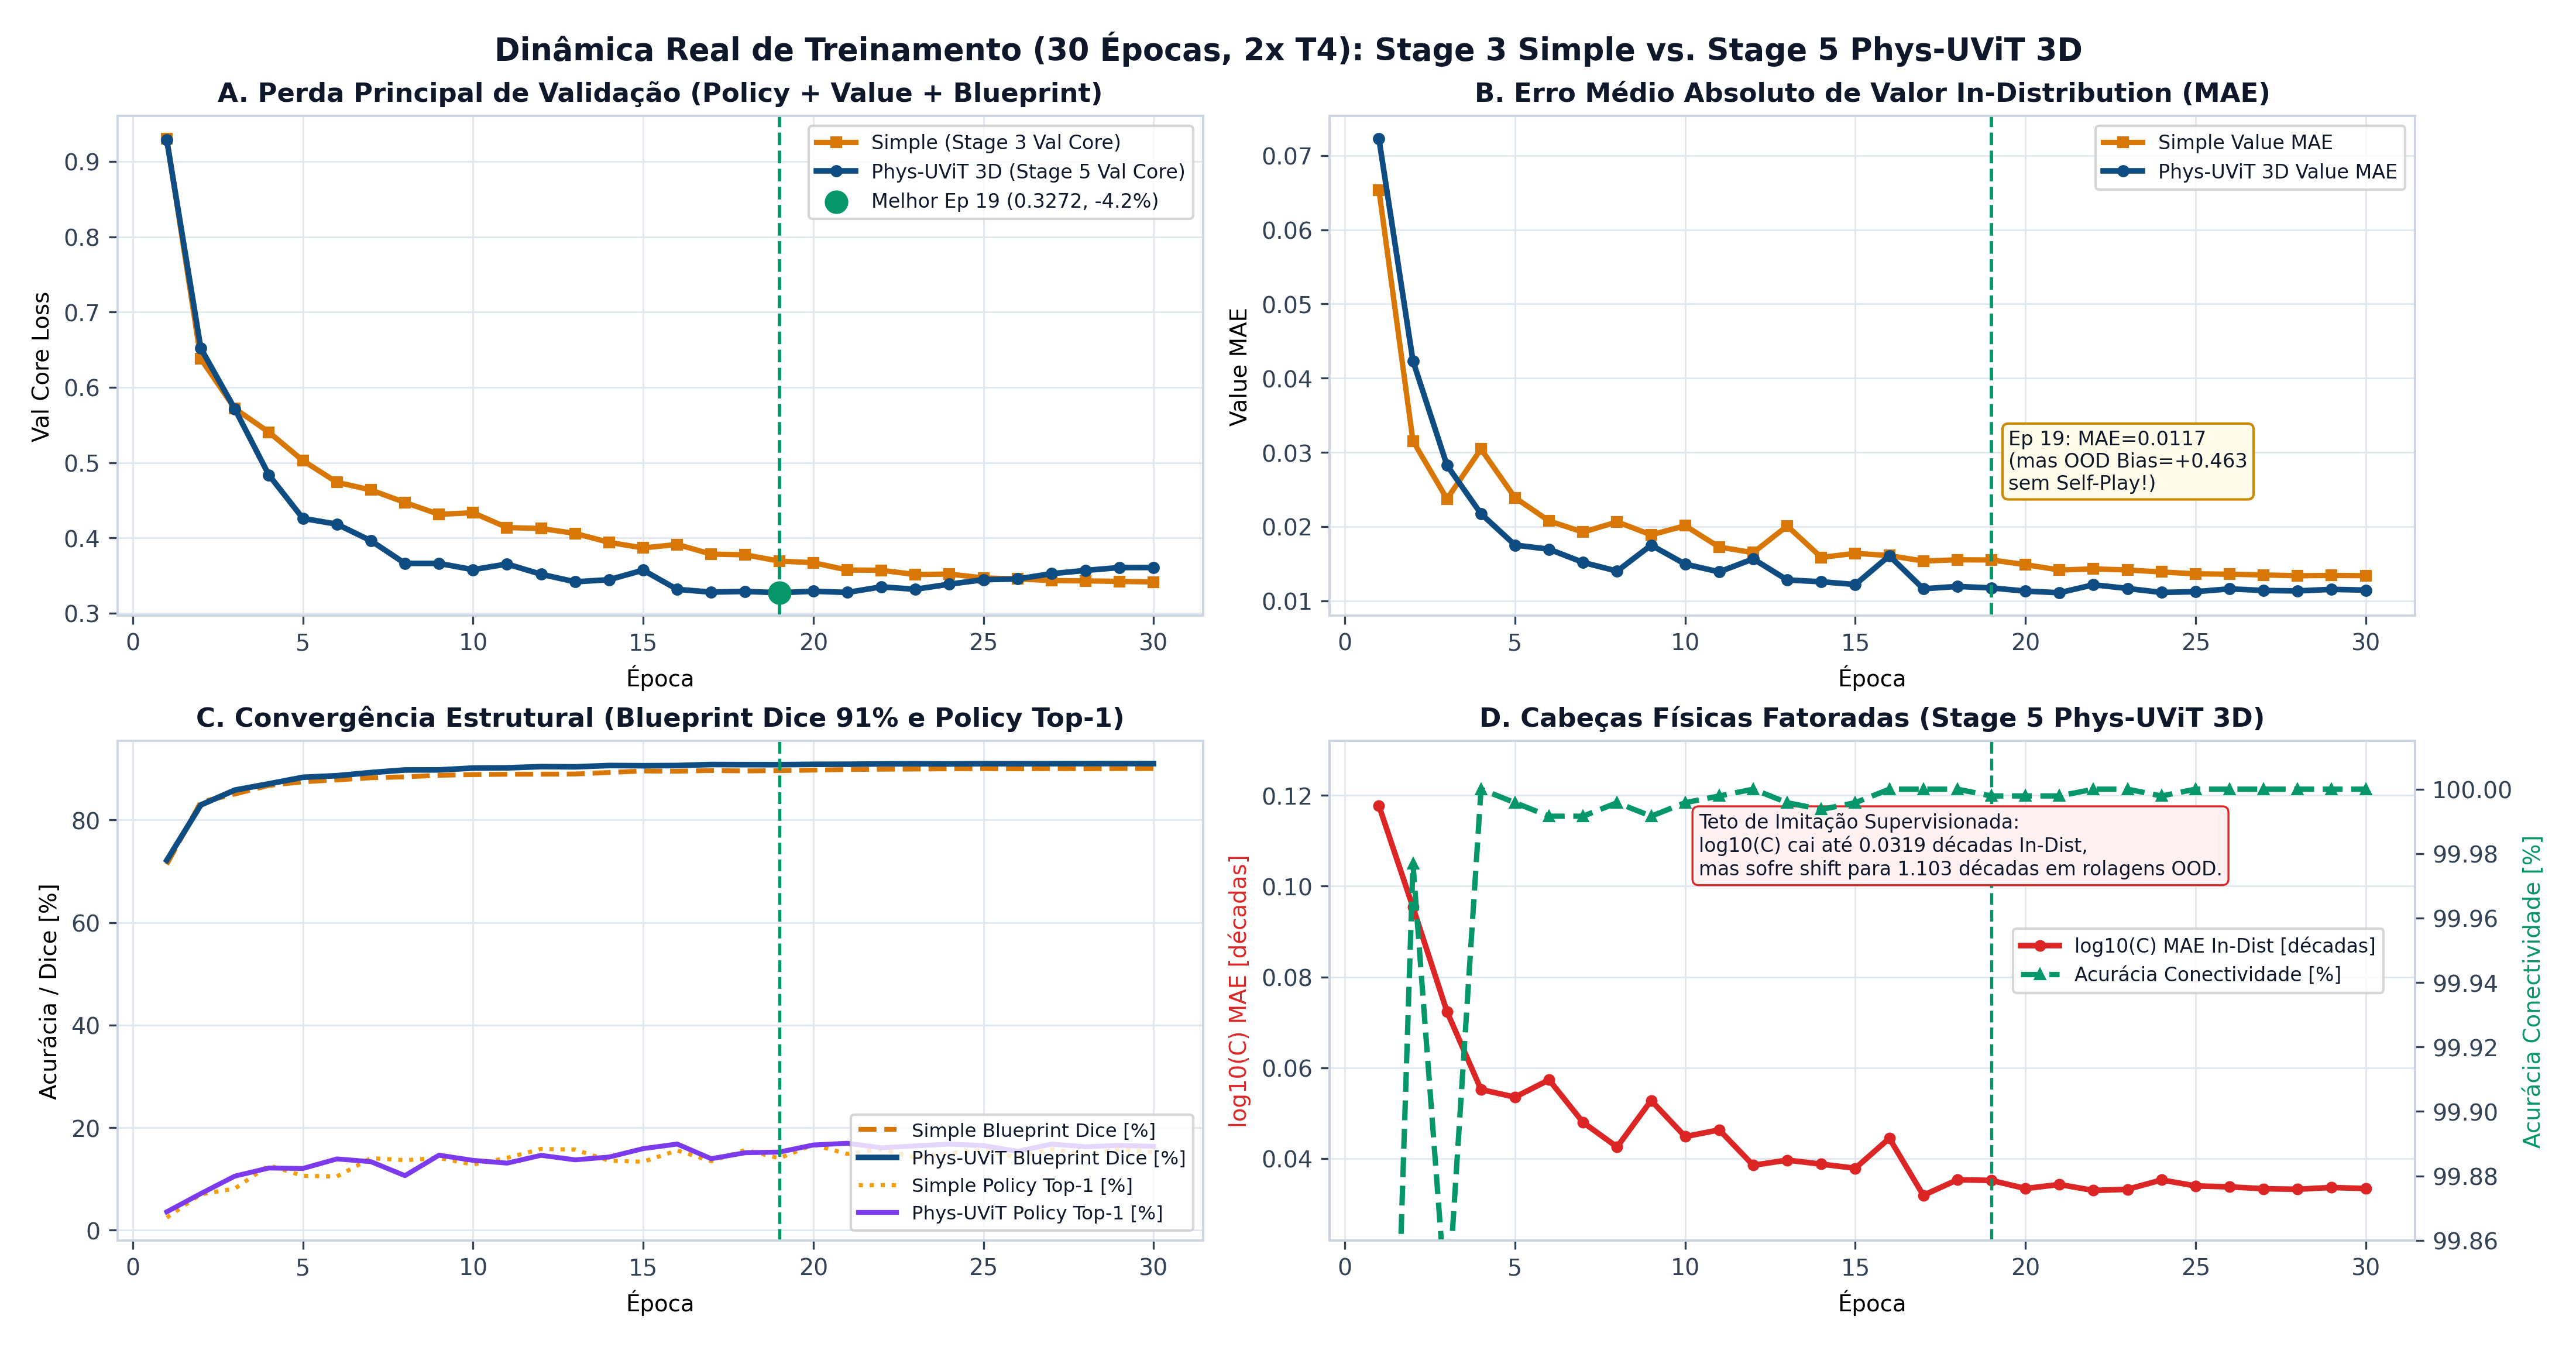
\includegraphics[width=\textwidth]{fig08_training_dynamics_stage3_vs_stage5.png}
\caption{Curvas reais das $30$ épocas de treinamento (\texttt{2x T4}) comparando \texttt{Simple Stage 3} e \texttt{Phys-UViT 3D Stage 5}: convergência de perdas (A), MAE de valor (B), Blueprint/Política (C) e o teto de imitação nas cabeças físicas (D).}
\label{fig:train-dyn}
\end{figure}

\begin{figure}[htbp]
\centering
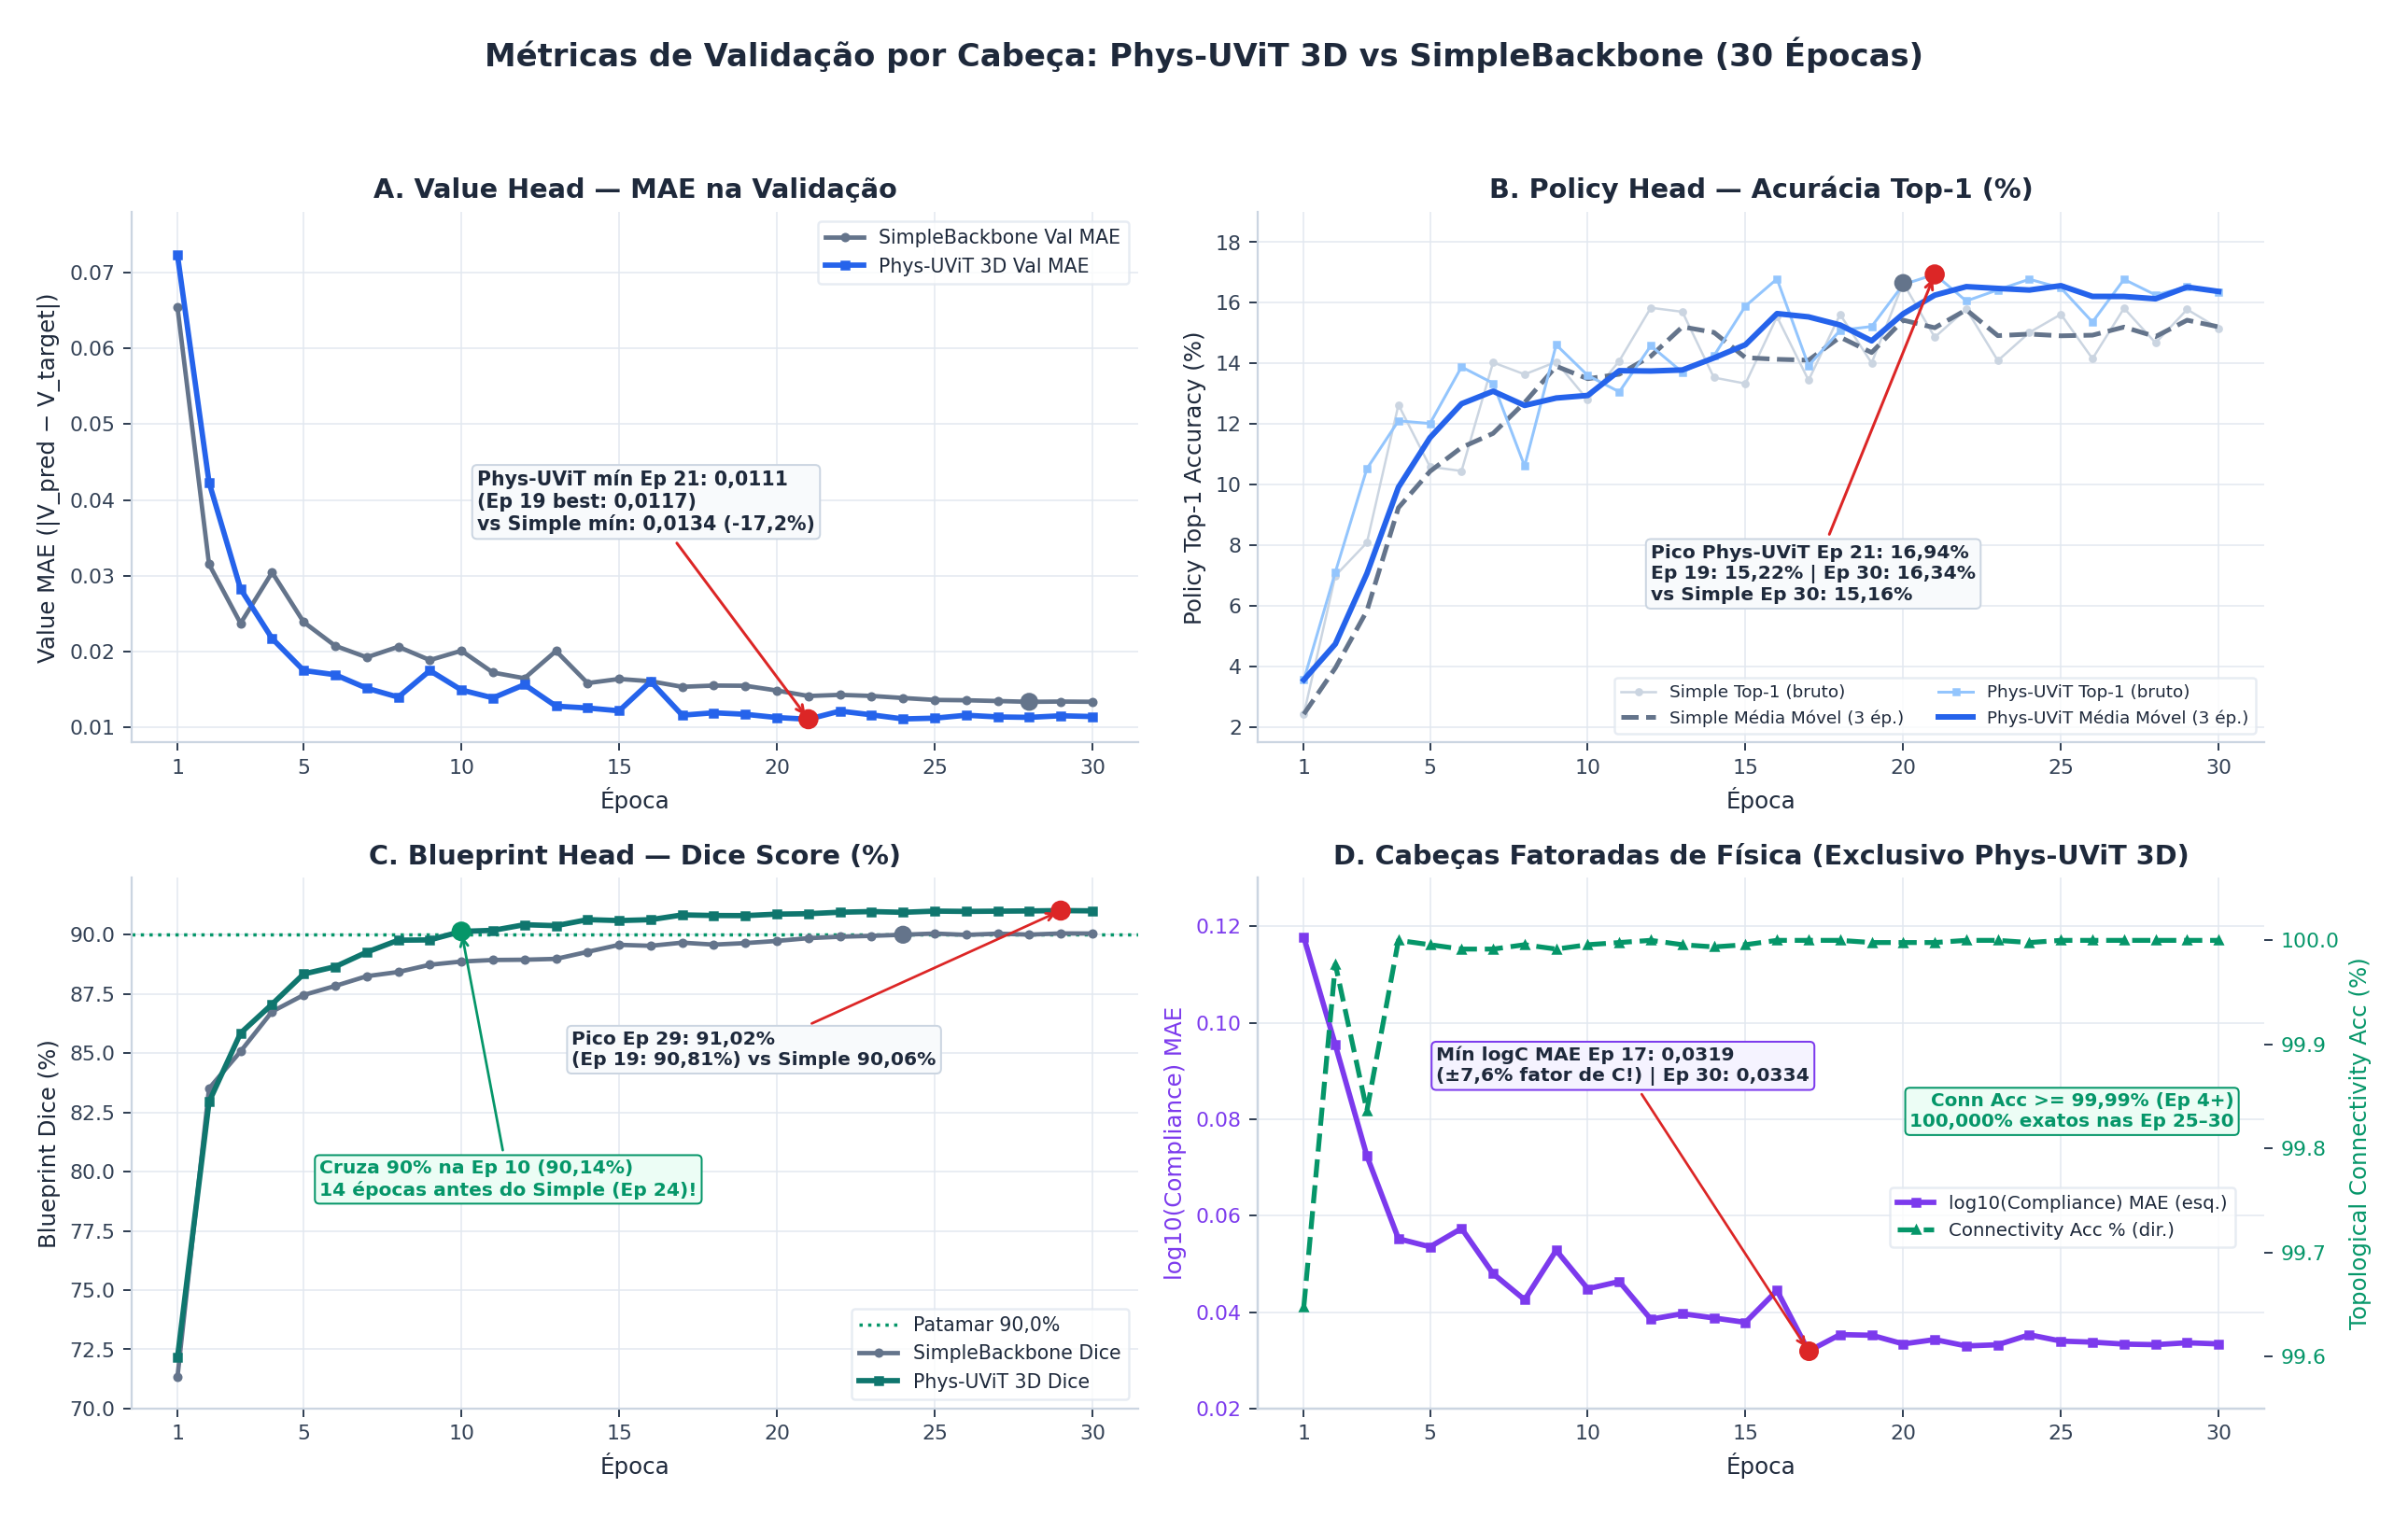
\includegraphics[width=\textwidth]{stage5_validation_heads_comparison.png}
\caption{Síntese comparativa das métricas de validação por cabeça no Stage 5 (\texttt{ep19}) versus \texttt{Stage 3} (\texttt{ep30}).}
\label{fig:val-heads}
\end{figure}

\begin{figure}[htbp]
\centering
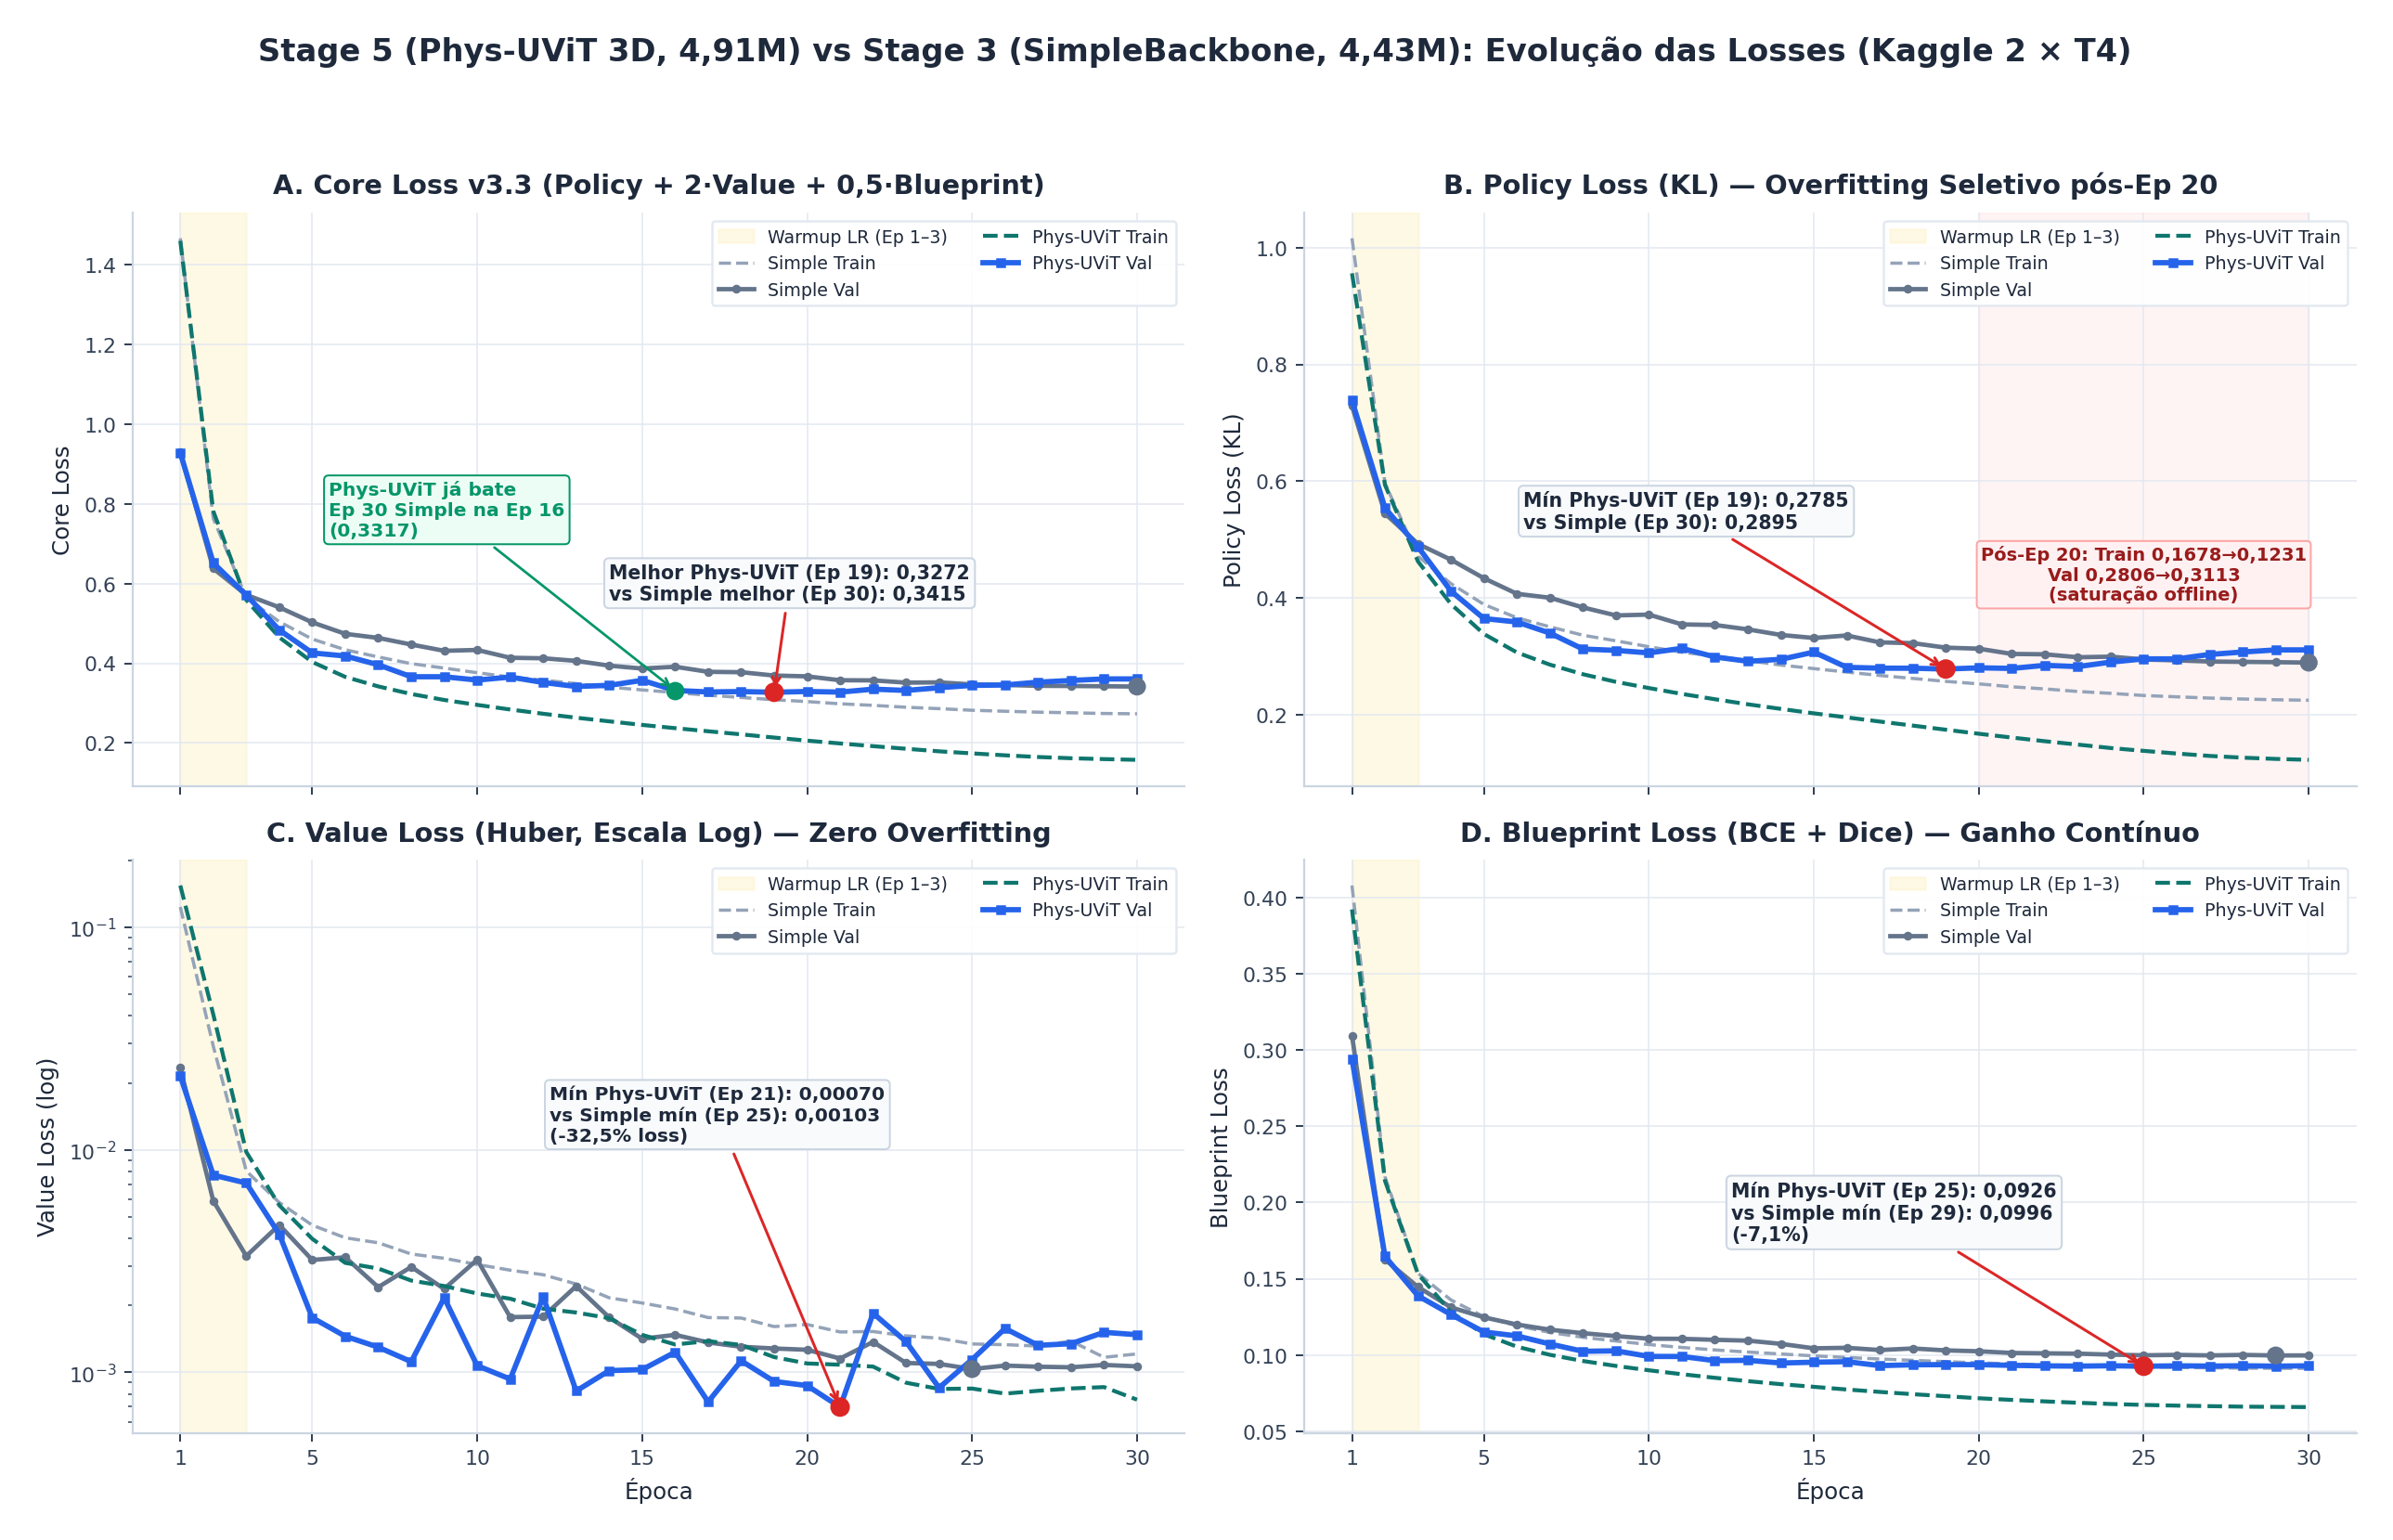
\includegraphics[width=\textwidth]{stage5_losses_comparison.png}
\caption{Evolução das componentes individuais de perda no treinamento do Stage 5 frente ao Stage 3.}
\label{fig:losses-comp}
\end{figure}

Em relação à compatibilidade de hardware (Figura~\ref{fig:hw-viab}), a \texttt{Phys-UViT 3D} permanece deliberadamente otimizada para \textbf{GPUs CUDA} em vez de \textbf{TPUs (\texttt{XLA})}: primeiro, camadas \texttt{Conv3d} de poucos canais e \texttt{GroupNorm} apresentam baixa eficiência nas unidades matriciais $128\times 128$ de TPUs; segundo, o treinamento multi-resolução com \texttt{BucketedResolutionBatchSampler} no Stage 6 alterna shapes de tensor entre mini-lotes, disparando recompilações XLA custosas; terceiro, a coleta de Self-Play acopla lotes pequenos ($B=1..8$) em tempo real com \texttt{PyAMG} e \texttt{SciPy} rodando na CPU, onde a baixa latência PCIe CPU--GPU de estações CUDA (\texttt{2x T4}, \texttt{A100}, \texttt{H100}) mostra-se amplamente superior.

\begin{figure}[htbp]
\centering
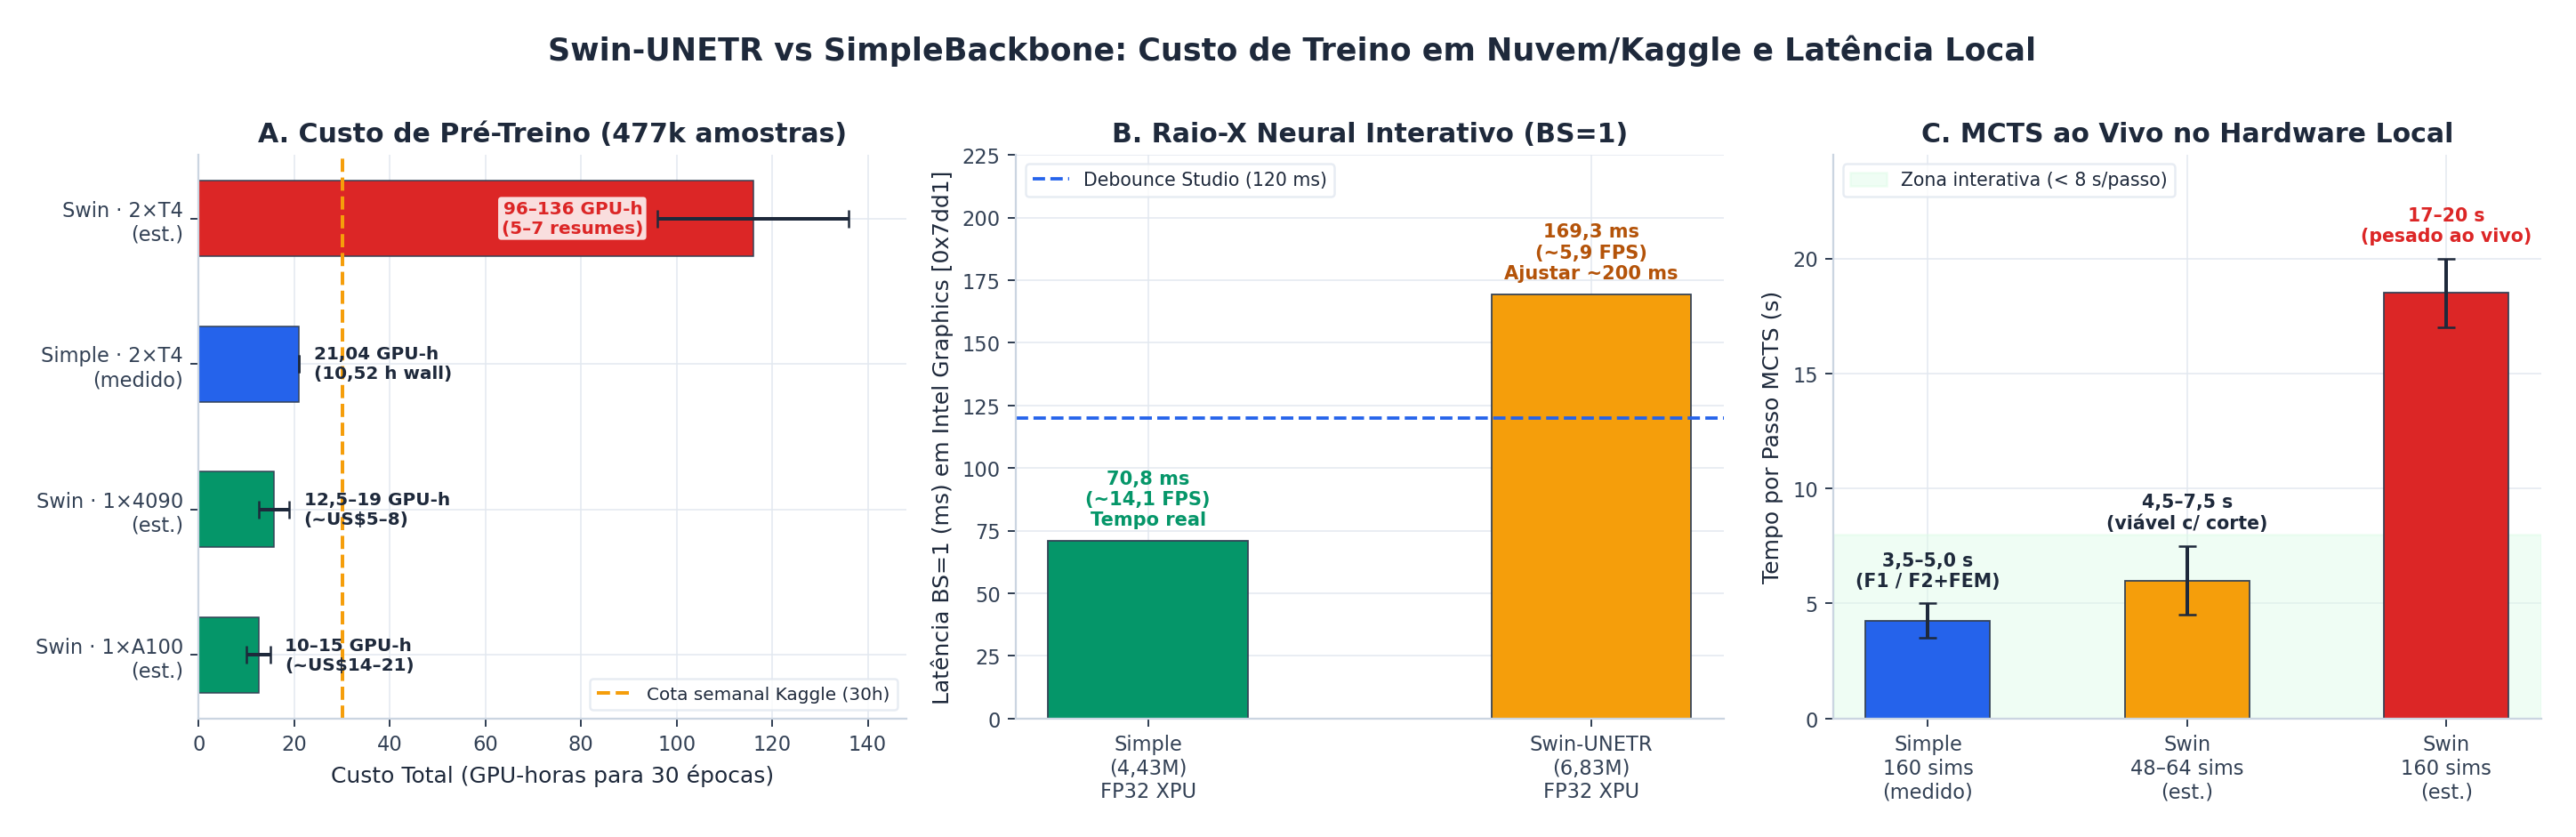
\includegraphics[width=\textwidth]{hardware_cost_latency_viability.png}
\caption{Análise de viabilidade computacional por plataforma de hardware (\texttt{T4}, \texttt{A100}, \texttt{H100}, \texttt{NPU}), latência de inferência e throughput de busca.}
\label{fig:hw-viab}
\end{figure}

\chapter{Autópsia Forense do Stage 5C: Ver Para Crer no Gap de \texttt{41x}}
\chaptermark{Autópsia Forense do Stage 5C}

\section{Placar Completo na Suíte Canônica \texttt{S1..S6}}

Submetendo \texttt{Phys-UViT ep19} ao teste completo de episódios reais em \texttt{S1..S6} ($160$ simulações MCTS, até $30\times 8 = 240$ edições na Fase 2, avaliados no oráculo \texttt{dolfinx}), emergiu o contraste agudo sintetizado na Tabela~\ref{tab:stage5c-full} e nas Figuras~\ref{fig:real-3d} e \ref{fig:stage5-eval-scores}.

\begin{table}[htbp]
\centering
\caption{Avaliação completa Stage 5C nos cenários canônicos \texttt{S1..S6} (\texttt{dolfinx}): \texttt{ep2}, \texttt{ep30}, \texttt{Phys-UViT ep19}, \texttt{SIMP\_bin} e \texttt{SIMP\_cont}.}
\label{tab:stage5c-full}
\resizebox{\textwidth}{!}{%
\begin{tabular}{@{}lccccc@{}}
\toprule
Cenário & \texttt{Simple ep2} ($V/C/\text{Score}$) & \texttt{Simple ep30} ($V/C/\text{Score}/I_y/P_1$) & \texttt{Phys-UViT ep19} ($V/C/\text{Score}/I_y/P_1/\text{hol}$) & \texttt{SIMP\_bin} ($V/C/\text{Score}$) & \texttt{SIMP\_cont} ($V/C/\text{Score}/I_y$) \\
\midrule
\texttt{S1} (\texttt{FULL}, $x=63,y=16$) & $9.46\%/62{,}228/-0.164$ & $10.69\%/23{,}348/-0.046/0.035/48$ & $8.89\%/24{,}546/-0.029/0.044/38/0.169$ & $10.13\%/21{,}083/\mathbf{-1.000}$ & $12.83\%/\mathbf{596.4}/+0.458/0.508$ \\
\texttt{S2} (\texttt{FULL}, $x=63,y=6$) & $13.18\%/17{,}347/-0.063$ & $11.04\%/22{,}039/-0.087\text{ (2 isl)}/49$ & $9.47\%/16{,}859/\mathbf{+0.034}/0.082/41/0.003$ & $10.91\%/48{,}847/\mathbf{-1.000}$ & $13.04\%/\mathbf{600.4}/+0.452/0.518$ \\
\texttt{S3} (\texttt{FULL}, $x=44,y=24$) & $7.32\%/55{,}015/-0.092$ & $7.96\%/10{,}402/+0.145\text{ (8.6\% ovX)}/34$ & $7.71\%/7{,}600/\mathbf{+0.199}/0.050/32/0.003$ & $12.78\%/25{,}127/\mathbf{-1.000}$ & $13.84\%/\mathbf{249.6}/+0.565/0.380$ \\
\texttt{S4} (\texttt{RAIL}, $x=58,y=16$) & $8.11\%/85{,}583/-0.179$ & $10.73\%/15{,}806/+0.012\text{ (5.3\% ovX)}/48$ & $6.93\%/68{,}916/-0.117/\mathbf{0.008}/28/0.000$ & $11.13\%/254{,}506/\mathbf{-1.000}$ & $13.14\%/\mathbf{789.1}/+0.408/\mathbf{0.494}$ \\
\texttt{S5} (\texttt{RAIL}, $x=52,y=11$) & $7.91\%/46{,}687/-0.082$ & $9.47\%/13{,}747/+0.065\,(z_c{=}2.99)/41$ & $7.65\%/18{,}336/\mathbf{+0.067}\,(z_c{=}3.32)/32$ & $12.54\%/70{,}139/\mathbf{-1.000}$ & $13.70\%/\mathbf{420.5}/+0.489/0.431$ \\
\texttt{S6} (\texttt{FULL}, $x=36,y=16$) & $4.98\%/36{,}020/+0.031$ & $7.28\%/5{,}732/+0.253\text{ (5.2\% ovX)}/31$ & $5.37\%/5{,}617/\mathbf{+0.303}/0.017/20/0.011$ & $14.41\%/6{,}801/+0.048$ & $14.52\%/\mathbf{102.0}/+0.684/0.341$ \\
\midrule
\textbf{MÉDIA \texttt{S1..S6}} & $8.49\%/50{,}480/-0.092$ & $9.53\%/15{,}179/+0.057/4.43\%\text{ ovX}/41.8$ & $\mathbf{7.67\%/23{,}646/+0.076/0.00\%\text{ ovX}/31.8}$ & $\mathbf{-0.825}$ ($5/6$ falhas) & $13.51\%/\mathbf{459.7}/\mathbf{+0.509}$ \\
\bottomrule
\end{tabular}%
}
\end{table}

\begin{figure}[htbp]
\centering
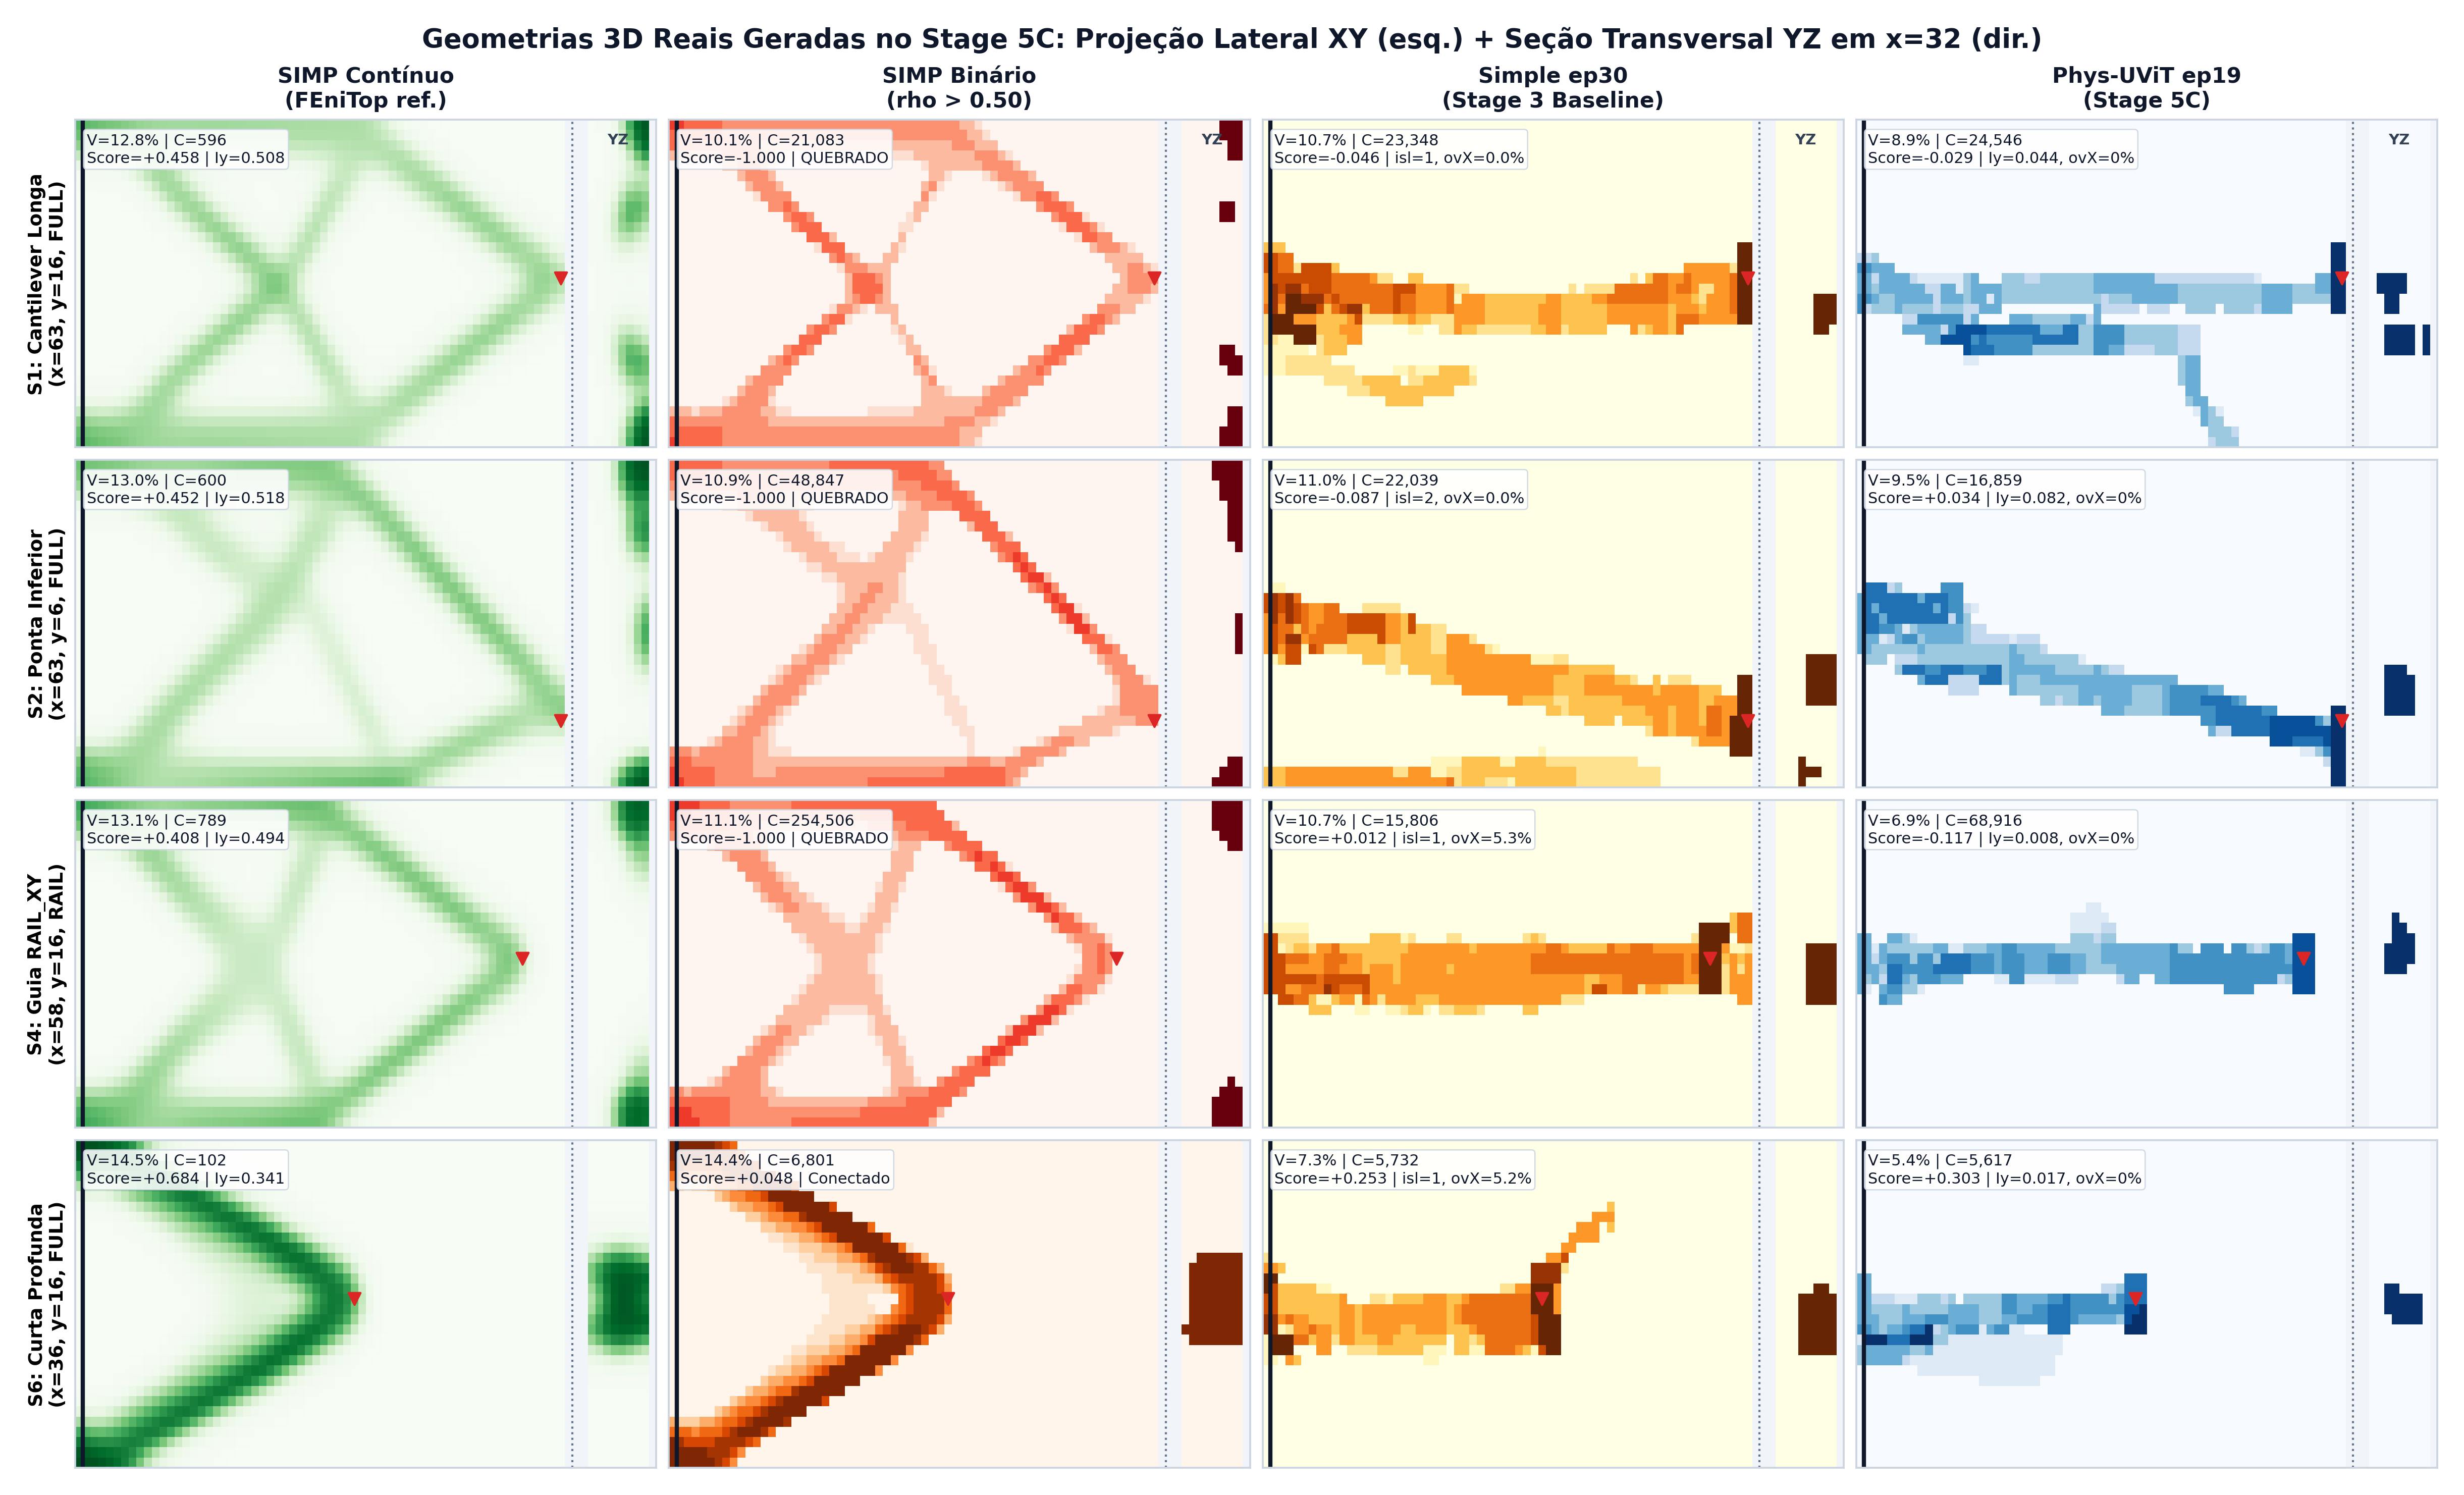
\includegraphics[width=\textwidth]{fig06_real_3d_geometries_comparison.png}
\caption{Geometrias 3D reais extraídas do banco \texttt{eval\_inference\_v4\_stage5.db} para \texttt{S1, S2, S4, S6}: projeção lateral $XY$ (esquerda) e seção transversal $YZ$ no meio do vão $x=32$ (direita). Observa-se imediatamente o colapso do \texttt{SIMP\_bin} na carga, as ilhas/\emph{overshoot} de \texttt{ep30} e o perfil central excessivamente raso ($I_y = 0.008$ em \texttt{S4}) da \texttt{Phys-UViT ep19}.}
\label{fig:real-3d}
\end{figure}

\begin{figure}[htbp]
\centering
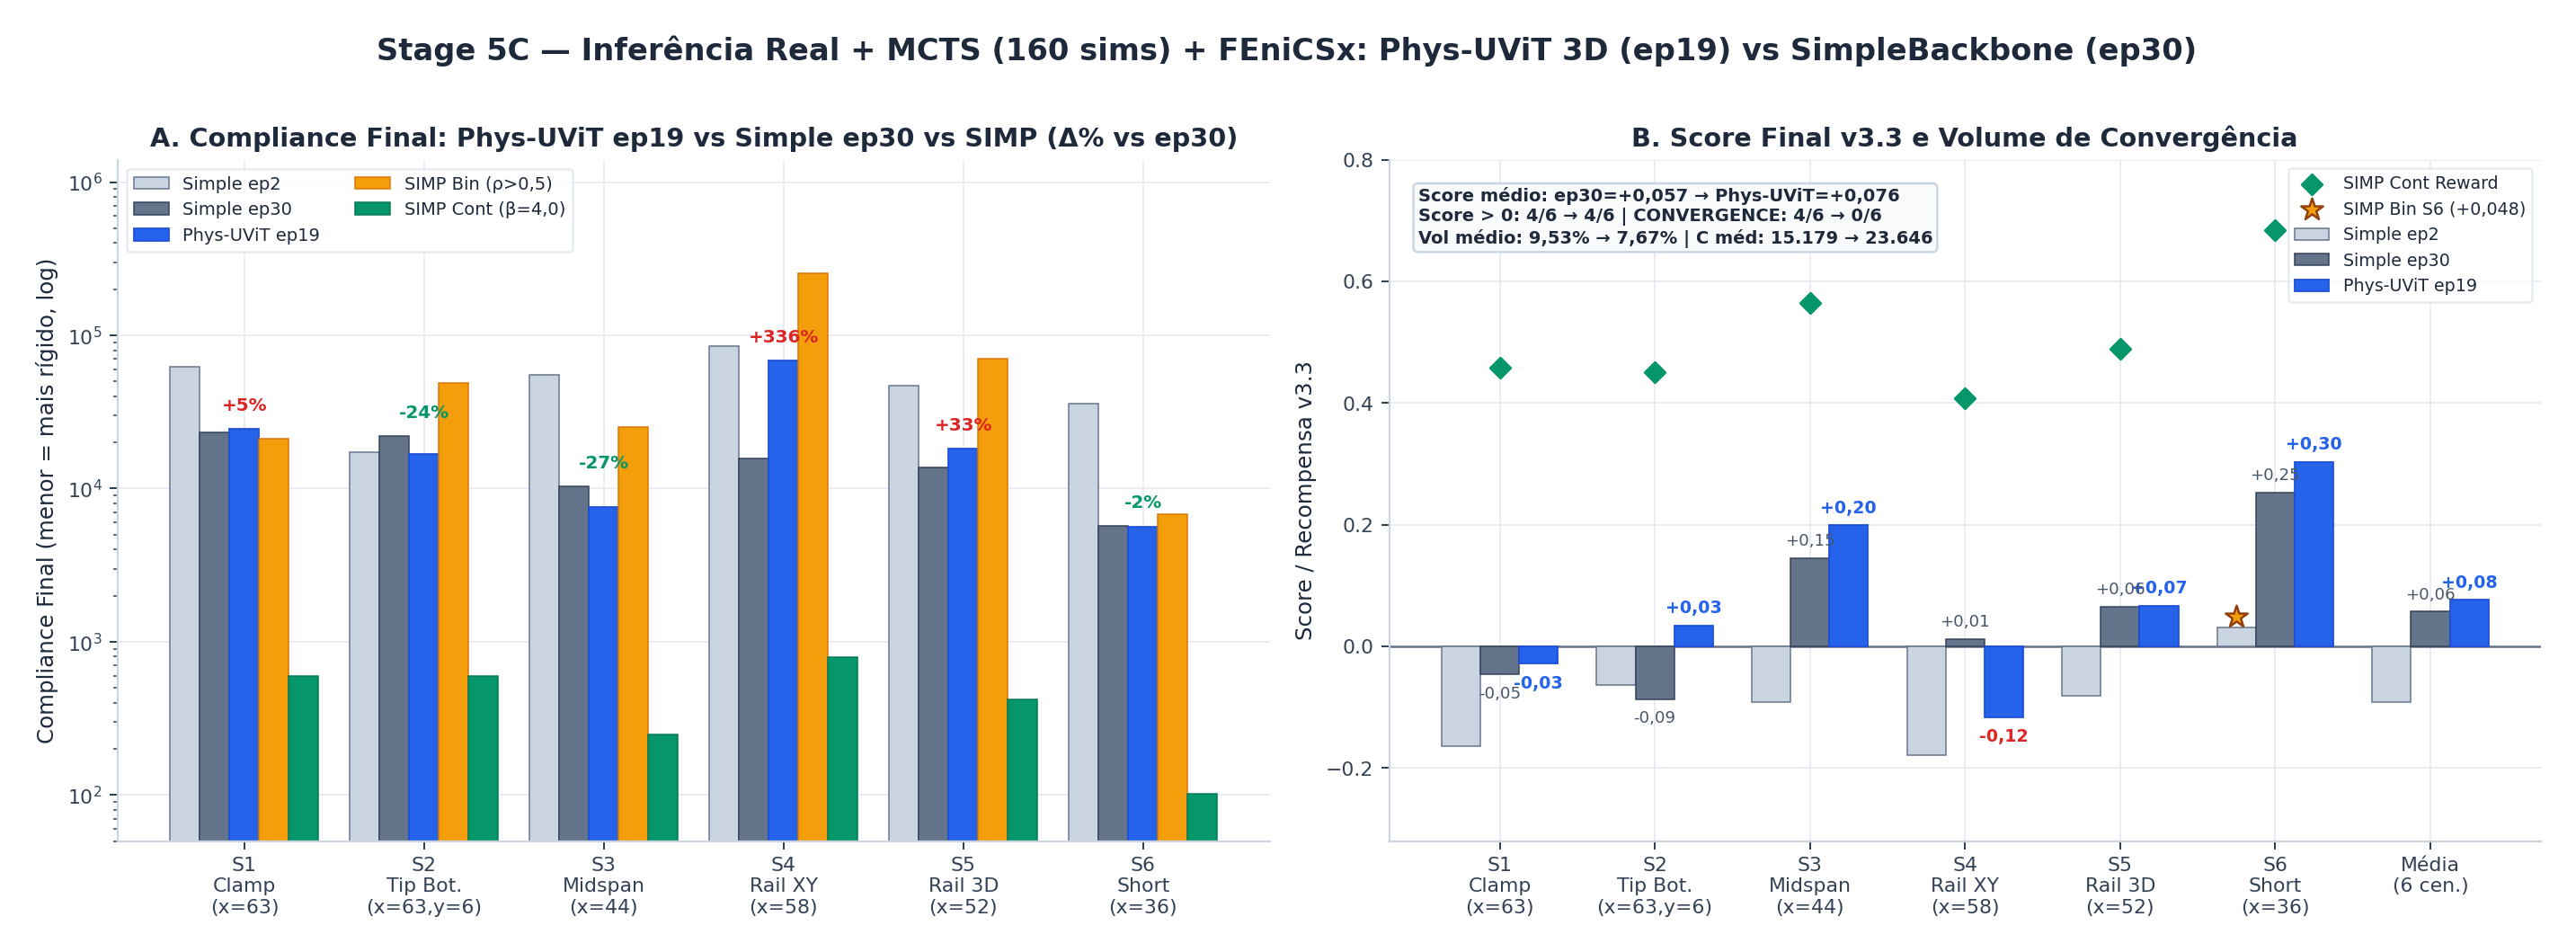
\includegraphics[width=\textwidth]{stage5_eval_compliance_score.png}
\caption{Comparativo direto por cenário (\texttt{S1..S6}) de compliance e Score \texttt{v3.3} no Stage 5C.}
\label{fig:stage5-eval-scores}
\end{figure}

A leitura visual da Figura~\ref{fig:real-3d} esclarece tudo o que as médias escondem. A \texttt{Phys-UViT ep19} venceu o \texttt{Simple ep30} em $5/6$ cenários ($+0.076$ vs. $+0.057$, $+33.3\%$), reduziu passos em Fase 1 ($31.8$ vs. $41.8$), \textbf{eliminou completamente o \emph{overshoot} em $X$ ($0.00\%$ em $6/6$ casos vs. $4.43\%$)}, curou a fratura dupla do \texttt{ep30} em \texttt{S2} e bateu \texttt{SIMP\_bin} em $6/6$ cenários (destaque para \texttt{S6}: $+0.303$ vs. $+0.048$ com menos de $40\%$ da massa!). Ainda assim, expôs pontos concretos de melhora: uma ilha residual solta em \texttt{S1} (\texttt{isl=2}, $-0.020$), centroide em $Z$ ainda centrado em \texttt{S5} ($3.32$ vs. $0.99$), e um abismo de $41.1\times$ em compliance frente ao \texttt{SIMP\_cont} em \texttt{S1} ($40.6\times$ em média geométrica).

\section{Momento Eureka \#4: Experimento Controlado no \texttt{dolfinx}}

Para testar se a representação binária $0/1$ carregava alguma limitação física intrínseca frente ao contínuo, conduzimos experimentos controlados diretos em \texttt{dolfinx} no cenário \texttt{S1} (Tabela~\ref{tab:dolfinx-s1}).

\begin{table}[htbp]
\centering
\caption{Experimento empírico controlado no \texttt{dolfinx} em \texttt{S1}: testemunhas discretas $0/1$ superam \texttt{SIMP\_cont}, enquanto colar artificial não altera \texttt{Phys-UViT ep19}.}
\label{tab:dolfinx-s1}
\resizebox{\textwidth}{!}{%
\begin{tabular}{@{}lcccc@{}}
\toprule
Configuração Estrutural Testada em \texttt{S1} & Volume $V$ & Conectada? & Compliance $C$ [J] & Score \texttt{v3.3} \\
\midrule
Bloco Sólido $100\%$ (limite físico teórico do cubo) & $100.00\%$ & Sim & $33.68$ & --- \\
\textbf{\texttt{SIMP thr > 0.50} + colar sólido 1-voxel na carga} & $10.35\%$ & \textbf{Sim} & $\mathbf{319.37}$ & $\mathbf{+0.615}$ \\
\textbf{Treliça Binária \texttt{0/1} pura (\texttt{fh=3, z=2..6, pad 1-vox})} & $15.37\%$ & \textbf{Sim} & $\mathbf{356.42}$ & $\mathbf{+0.473}$ \\
\texttt{SIMP Contínuo} (\texttt{FEniTop} referência) & $12.83\%$ & Sim & $596.42$ & $+0.458$ \\
Treliça Binária \texttt{0/1} (\texttt{fh=3}, patch exato sem colar) & $15.26\%$ & Sim & $3{,}948.45$ & $+0.110$ \\
\texttt{SIMP thr > 0.50} (patch exato sem colar) & $10.15\%$ & Sim & $7{,}382.40$ & $+0.142$ \\
\texttt{SIMP\_bin} puro (corte $\rho > 0.50$ sem proteção) & $10.13\%$ & Não & $21{,}083.35$ & $-1.000$ \\
\texttt{Phys-UViT ep19} (Stage 5C real) & $8.89\%$ & Sim & $24{,}546.42$ & $-0.029$ \\
\texttt{Phys-UViT ep19} + colar artificial de 1 voxel na carga & $8.89\%+$ & Sim & $24{,}546.42$ & $-0.029$ \\
\bottomrule
\end{tabular}%
}
\end{table}

Essa bateria prova dois fatos definitivos: primeiro, estruturas estritamente binárias $0/1$ atingem \textbf{rigidez superior e score superior ao \texttt{SIMP contínuo}} ($C = 356.42$ e $319.37\text{ J}$ contra $596.42\text{ J}$), porque todo voxel sólido opera a $100\%$ de $E_0$; segundo, acrescentar o colar de proteção na \texttt{Phys-UViT ep19} provocou \textbf{exatos $0.00\%$ de redução em compliance} nos cenários \texttt{S1}, \texttt{S4} e \texttt{S6}. Logo, a rede já domina o acoplamento local da carga.

\section{Os Quatro Gargalos Reais no Banco \texttt{eval\_inference\_v4\_stage5.db}}

A inspeção forense dos quadros individuais da Fase 2 revela exatamente o que prendeu o MCTS antes do Self-Play (Figuras~\ref{fig:ood-blindness} e \ref{fig:stage5-geom-cal}):

\begin{enumerate}
\item \textbf{Déficit flexional $I_y$ ($6.3\times$ a $63.1\times$):} como a Fase 1 priorizou conexões diretas ao longo do centro, o momento de inércia da peça gerada caiu para até $0.0078$ em \texttt{S4} (contra $0.4941$ no \texttt{SIMP\_cont}).
\item \textbf{Cegueira OOD de Valor e Compliance:} embora o classificador de conectividade \texttt{P(conn)} tenha generalizado com precisão absoluta ($0.00013$ em P1 $\to 1.00000$ em P2), fora da distribuição de warmup o modelo subestima $\log_{10} C$ em \textbf{$-1.103$ décadas} e superestima o Valor em \textbf{$+0.463$}. Pior ainda: em \texttt{S3}, \texttt{S4} e \texttt{S6}, o valor previsto $V_{\mathrm{net}}$ desce enquanto a física real $R_{\mathrm{FEM}}$ sobe ($r = -0.91, -0.80, -0.81$), guiando o MCTS com uma bússola invertida!
\item \textbf{Paralisia Cirúrgica de Remoção:} em todos os $6$ episódios combinados foram registradas \textbf{$1{,}435$ adições ($99.65\%$) contra apenas $5$ remoções ($0.35\%$)}, inviabilizando o vazamento do miolo neutro (\texttt{hollow\_ratio} $= 0.003$ em \texttt{S2} contra $0.582$ no \texttt{SIMP\_cont}).
\item \textbf{Teto de $240$ edições ($30\times 8$):} um orçamento de $1.46\%$ da grade não permite expandir abas afastadas e esculpir treliças após a conexão inicial.
\end{enumerate}

\begin{figure}[htbp]
\centering
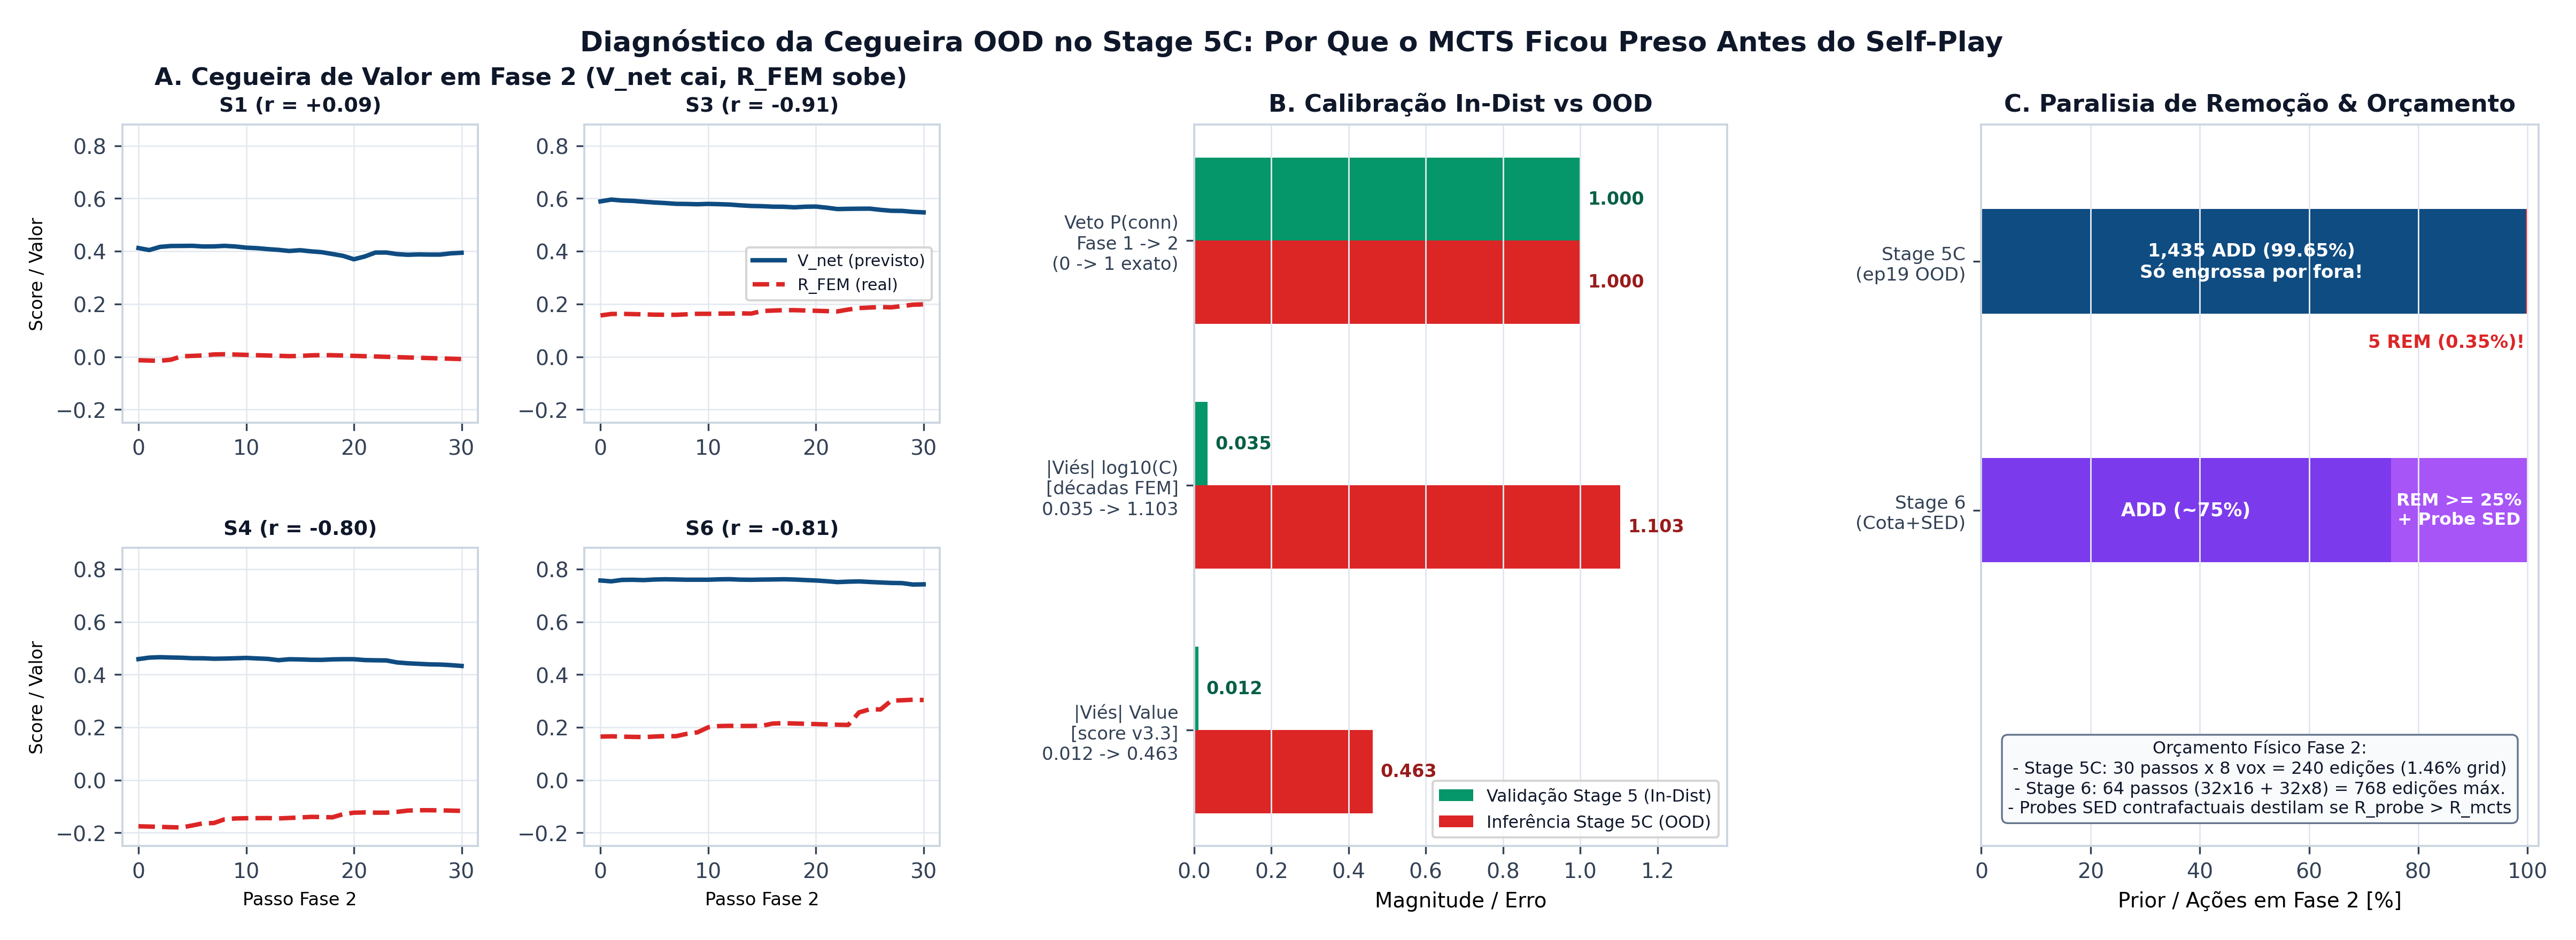
\includegraphics[width=\textwidth]{fig03_ood_blindness_diagnosis.png}
\caption{Diagnóstico da cegueira OOD no Stage 5C: correlação negativa entre $V_{\mathrm{net}}$ e $R_{\mathrm{FEM}}$ em \texttt{S3, S4, S6} (A), veto topológico perfeito vs. quebra de calibração em $\log_{10} C$/Valor (B) e paralisia \texttt{ADD/REM} + orçamento (C).}
\label{fig:ood-blindness}
\end{figure}

\begin{figure}[htbp]
\centering
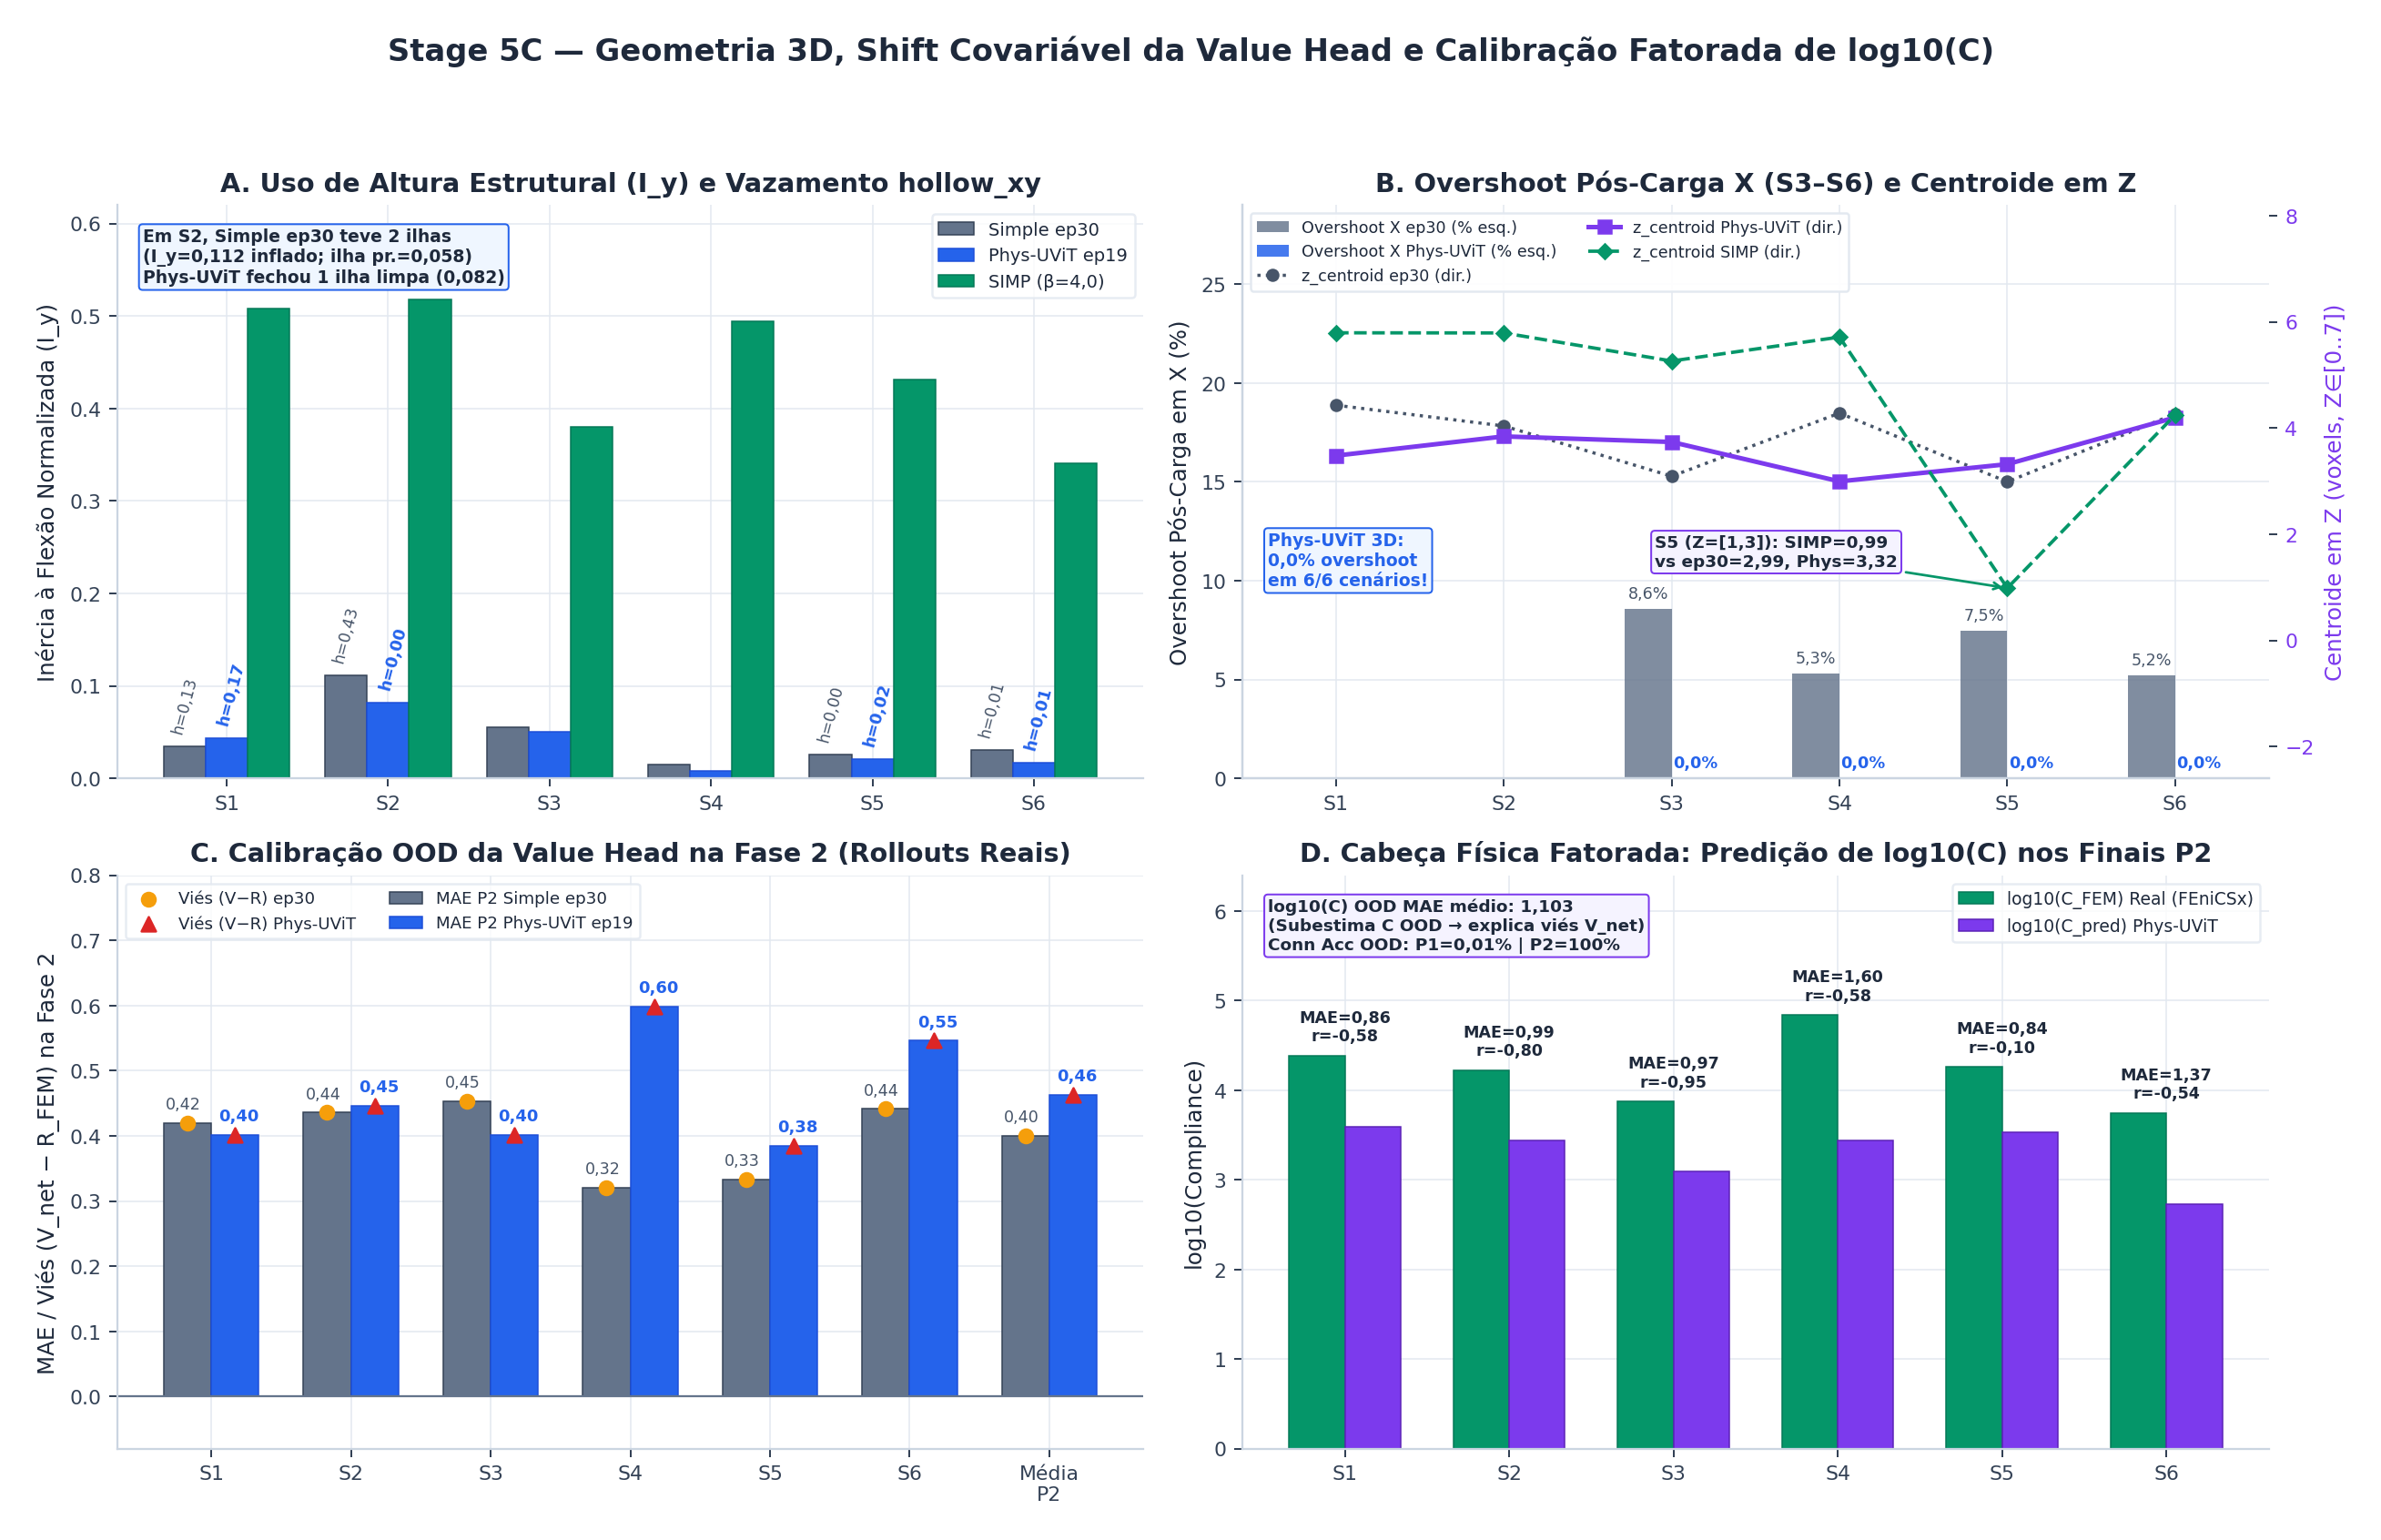
\includegraphics[width=\textwidth]{stage5_eval_geometry_and_calibration.png}
\caption{Métricas detalhadas de geometria (\emph{overshoot X}, inércia $I_y$, razão de vazamento) e calibração das cabeças por cenário no Stage 5C.}
\label{fig:stage5-geom-cal}
\end{figure}

\chapter{O Motor de Self-Play Fase 6: As 5 Alavancas Cirúrgicas e a Perda Multi-Cabeça}
\chaptermark{O Motor de Self-Play Fase 6}

\section{Ligando Cada Mecanismo ao Respectivo Gargalo}

As cinco alavancas codificadas no Stage 6 atacam um a um os quatro pontos cegos diagnosticados acima, fechando o ciclo entre busca em árvore, física exata e atualização neural:

\subsection*{Alavanca 1 — Oráculo \texttt{fast\_amg} + Supervisão Densa por \texttt{SED\_e}}
Em \texttt{runner.py}, cada passo conectado de Fase 2 invoca \texttt{evaluate\_main\_island(..., backend="fast\_amg", compute\_sed=True)}, gerando simultaneamente $R_{\mathrm{FEM}}(t)$, $\log_{10} C_{\mathrm{FEM}}(t)$ e o campo tridimensional $\mathrm{SED}_e$ armazenado em \texttt{sed\_map\_blob}. A Figura~\ref{fig:sed-surgery} mostra por que esse sinal é transformador: na \texttt{Phys-UViT ep19} (\texttt{S1}), o mapa $\mathrm{SED}_e$ revela uma perna pendente morta até $y=0$ com apenas $5.47\times 10^{-6}\text{ J}$ frente aos $314.9\text{ J}$ da garganta do engaste; na treliça binária $0/1$ de $356.4\text{ J}$, a energia distribui-se homogeneamente pelas abas externas. Supervisionar a cabeça \texttt{sed\_head} sobre $\log(1+\mathrm{SED}_e)$ ensina o gargalo Transformer a enxergar concentrações de tensão antes mesmo de agir.

\begin{figure}[htbp]
\centering
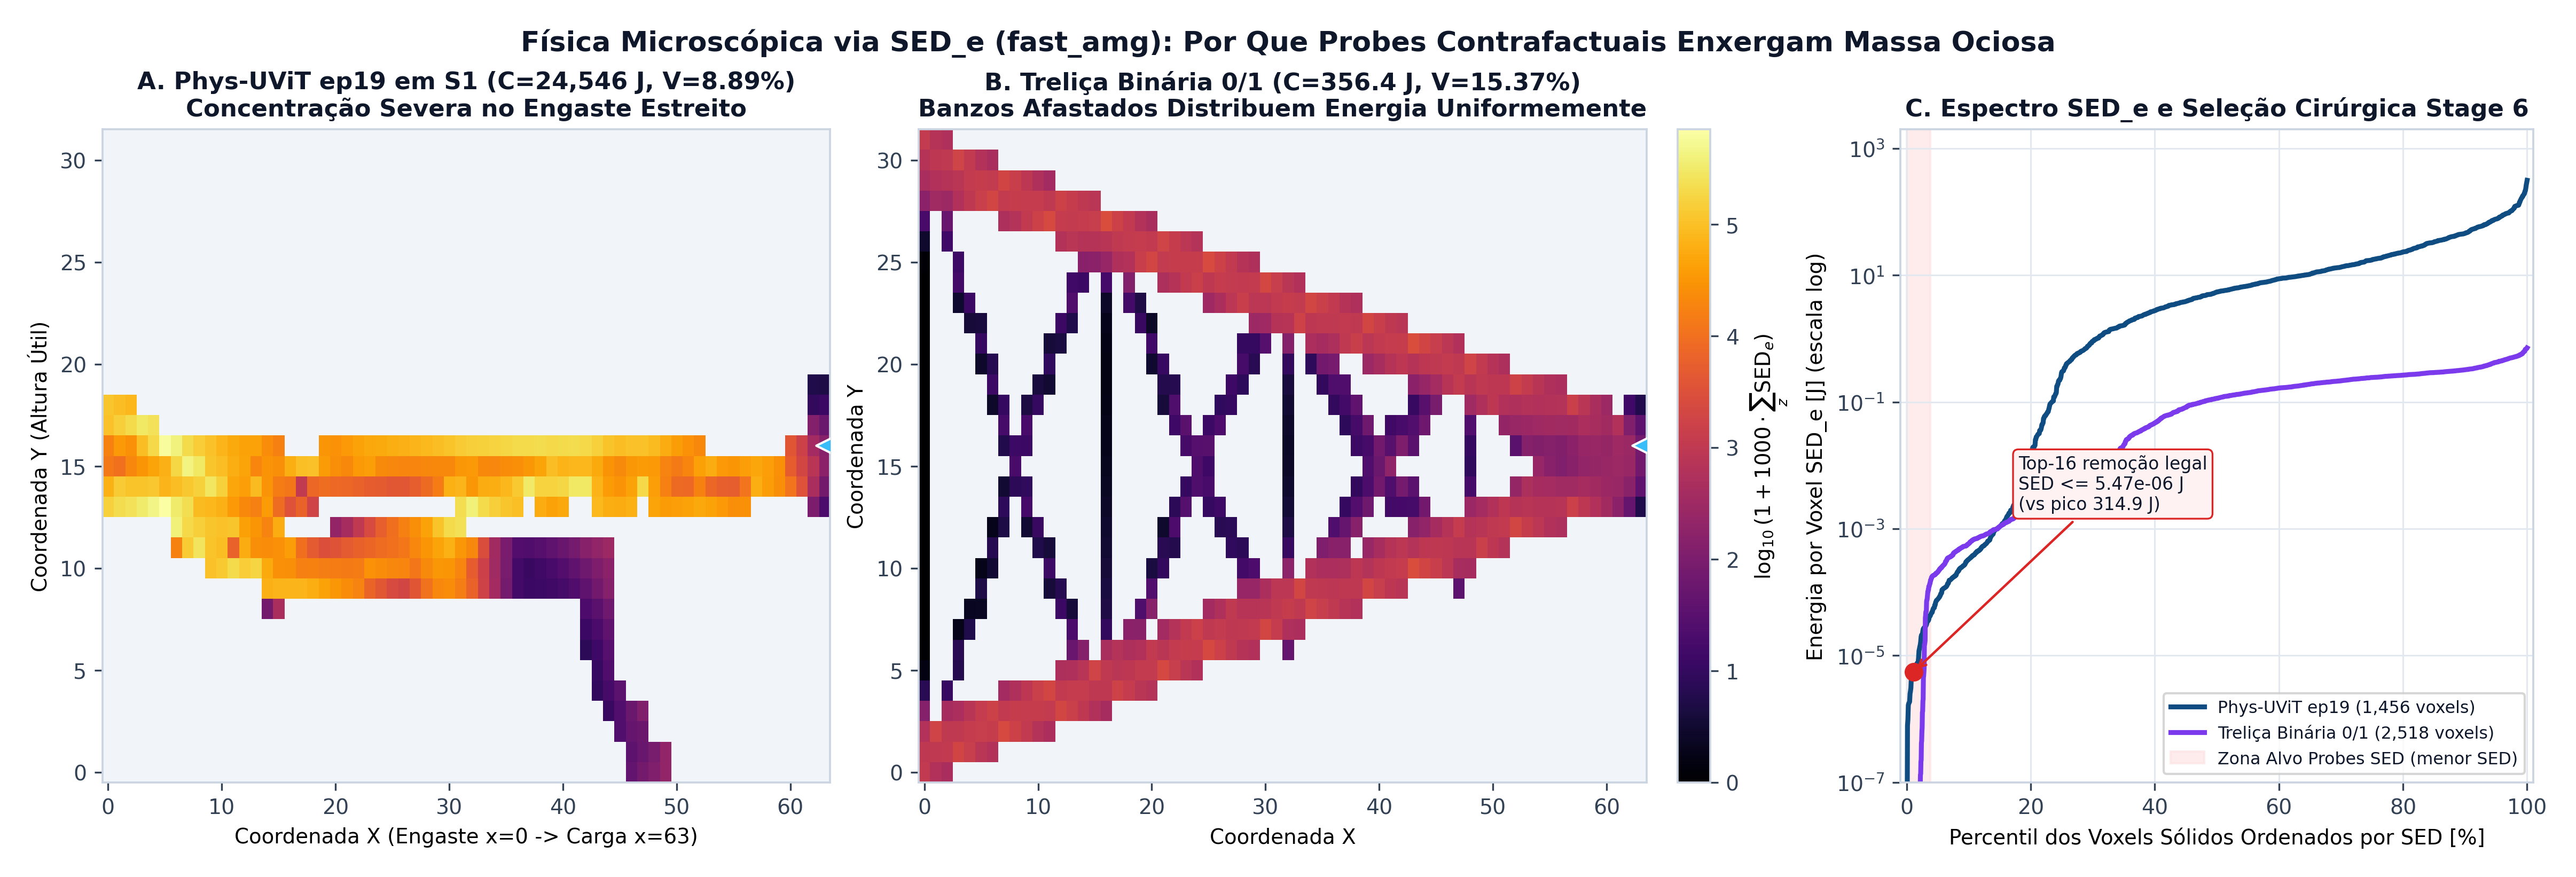
\includegraphics[width=\textwidth]{fig07_sed_field_and_counterfactual_surgery.png}
\caption{Campos exatos de \texttt{SED\_e} (\texttt{fast\_amg}) em \texttt{S1}: concentração crítica no eixo estreito e perna morta na \texttt{Phys-UViT ep19} (A), distribuição equilibrada na treliça $0/1$ de $356.4\text{ J}$ (B) e espectro ordenado de seleção para os $16$ candidatos legais de remoção em probes contrafactuais (C).}
\label{fig:sed-surgery}
\end{figure}

\subsection*{Alavanca 2 — Exploração Precoce em Fase 1 + PBRS Distância}
Para quebrar a atração precoce pela barra central reta, os primeiros $12$ passos da Fase 1 (\texttt{p1\_explore\_steps=12}) elevam a temperatura de seleção para $1.35$ e a fração de ruído de Dirichlet para $0.35$. Simultaneamente, o potencial euclidiano $w_{\mathrm{dist}}=0.25$ garante que essa exploração diversificada encontre caminhos viáveis mesmo diante de engastes inéditos ou obstáculos \texttt{keep-out} até a consolidação pela rede na geração $5$.

\subsection*{Alavanca 3 — Desbloqueio de Remoção, Orçamento $16 \to 8$ e \emph{Probes SED Contrafactuais}}
Em \texttt{MCTSNode.expand}, os parâmetros \texttt{min\_remove\_candidates=16} e \texttt{remove\_prior\_floor=0.25} garantem que ao menos $16$ remoções legais integrem o \texttt{top\_k} da Fase 2 com massa mínima de $25\%$ dos priors (renormalizada para $1.0$). O orçamento de Fase 2 estende-se para $64$ passos escalonados: $32$ passos com micro-lote $16$ (até $512$ adições/remoções estruturais largas) seguidos de $32$ passos com micro-lote $8$ (até $256$ refinamentos cirúrgicos, totalizando $768$ edições). Ademais, em $50\%$ dos passos com $V \ge 5.5\%$, o runner dispara um probe virtual removendo os voxels legais com menor $\mathrm{SED}_e$ sem desviar o episódio, registrando o resultado exato na tabela \texttt{fem\_probes} para calibrar \texttt{FactoredValueHead}, \texttt{log\_c\_head} e \texttt{sed\_head}.

\subsection*{Alavanca 4 — Função de Perda Composta Multi-Cabeça (\texttt{trainer.py})}
Para que o ajuste fino calibrado não distorça as representações globais nem deixe cabeças auxiliares desbalanceadas, cada lote em \texttt{scripts/train\_selfplay\_step.py} otimiza a perda composta com mascaramento independente por amostra (\texttt{policy\_mask}, \texttt{blueprint\_mask}, \texttt{compliance\_mask}, \texttt{conn\_mask}, \texttt{sed\_mask}). Dessa forma, amostras do Warmup (desprovidas de mapa denso \texttt{sed\_target}), estados intermediários da Fase 1 (sem compliance definida) e registros de \texttt{fem\_probes} (que calibram física sem atuar diretamente sobre \texttt{policy\_mask}) contribuem rigorosamente apenas onde possuem ground truth exato:
\begin{equation}
\mathcal{L}_{\mathrm{total}} =
\underbrace{1.0\,\mathcal{L}_{\mathrm{KL}}}_{\mathrm{Policy}}
+ \underbrace{2.0\,\mathcal{L}_{\mathrm{Huber}}^{(w_{\mathrm{neg}}=1.5)}}_{\mathrm{Value}}
+ \underbrace{0.25\,\mathcal{L}_{\mathrm{BP}}}_{\mathrm{Blueprint}}
+ \underbrace{0.35\,\mathcal{L}_{\log C}}_{\mathrm{Rigidez}}
+ \underbrace{0.25\,\mathcal{L}_{\mathrm{BCE}}}_{\mathrm{Conn}}
+ \underbrace{0.15\,\mathcal{L}_{\mathrm{SED}}}_{\mathrm{SED}}.
\end{equation}

\begin{table}[htbp]
\centering
\caption{Detalhamento das seis componentes da função de perda no ajuste fino misto Stage 6.}
\label{tab:stage6-losses}
\resizebox{\textwidth}{!}{%
\begin{tabular}{@{}llcl@{}}
\toprule
Componente & Definição Matemática (\texttt{float32} sob AMP) & Peso ($\lambda$) & Papel na Quebra da Cegueira OOD \\
\midrule
$\mathcal{L}_{\mathrm{KL}}$ & $\sum_a \pi_{\mathrm{MCTS}}(a)\log\frac{\pi_{\mathrm{MCTS}}(a)}{\mathrm{softmax}(z_{\mathrm{legal}})(a)}$, com \texttt{policy\_mask} & $1.00$ & Destila escolhas validadas pelo MCTS sob \emph{Advantage Gating} \\
$\mathcal{L}_{\mathrm{Huber}}^{(w_{\mathrm{neg}})}$ & SmoothL1 ($\beta=0.2$), multiplicando por $w_{\mathrm{neg}}=1.5$ se $V_{\mathrm{target}}\le 0$ & $2.00$ & Pune assimetricamente o falso otimismo em peças frágeis ou quebradas \\
$\mathcal{L}_{\mathrm{BP}}$ & $0.5\,\mathrm{BCEWithLogits} + 0.5\,\mathrm{SoftDice}$ (amostras do Warmup) & $0.25$ & Preserva o contorno geométrico suave do \texttt{SIMP} contra esquecimento \\
$\mathcal{L}_{\log C}$ & SmoothL1 ($\beta=0.2$) sobre $\log_{10} C_{\mathrm{FEM}}$ (estados conectados) & $0.35$ & Corrige o viés OOD de $-1.103$ décadas da \texttt{FactoredValueHead} \\
$\mathcal{L}_{\mathrm{BCE}}$ & \texttt{BCEWithLogits} sobre conectividade binária \texttt{is\_connected} & $0.25$ & Sustenta $100\%$ de precisão de veto topológico nos novos BCs \\
$\mathcal{L}_{\mathrm{SED}}$ & SmoothL1 ($\beta=0.5$) sobre $\log(1+\mathrm{SED}_e)$ no volume completo & $0.15$ & Ancora os mapas de atenção do Transformer no fluxo real de tensões \\
\bottomrule
\end{tabular}%
}
\end{table}

Para seleção de checkpoints ao longo das $6$ épocas por geração (\emph{cosine decay} após aquecimento linear, $\mathrm{lr}=5\times 10^{-5}$), monitora-se a perda de validação combinada equilibrando plasticidade em domínios novos e retenção estrutural: $0.70\,\mathcal{L}_{\mathrm{val,SelfPlay}} + 0.30\,\mathcal{L}_{\mathrm{val,Warmup}}$.

\subsection*{Alavanca 5 — \emph{Mixed Replay Buffer} (\texttt{60/40}), \emph{Advantage Gating} e Lotes Multi-Resolução}
Treinar exclusivamente sobre trajetórias de Self-Play apagaria a geometria global aprendida na \texttt{blueprint\_head} (\emph{catastrophic forgetting}). Por isso, \texttt{MixedReplayDataset} mistura $60\%$ de passos recentes de Self-Play com $40\%$ do dataset âncora \texttt{v3.3}, agrupados por dimensão espacial via \texttt{BucketedResolutionBatchSampler} ($0\%$ \emph{padding}) e submetidos às $16$ simetrias $D_4\times\mathbb{Z}_2$ preservando o alinhamento exato de \texttt{domain\_mask} e \texttt{sed\_target}. Além disso, durante a leitura de dados de Self-Play, aplica-se um filtro de \textbf{\emph{Advantage Gating}} ($\Delta V = V_{\mathrm{target}} - Q_{\mathrm{root}} \ge -0.005$): passos em que a ação executada deteriorou o retorno real retropropagado em comparação à estimativa da raiz têm \texttt{policy\_mask = 0} — a rede não imita erros da busca na cabeça de política, enquanto a cabeça de valor continua aprendendo exatamente por que aquela ação perdeu pontos.

\section{Anatomia Temporal de um Episódio Completo de Self-Play (\texttt{runner.py})}

Para visualizar todas as peças operando em harmonia, acompanhe a linha do tempo concreta de um único episódio Stage 6 típico no domínio \texttt{64x32x8}:
\begin{enumerate}
\item \textbf{Passos $0 \to 11$ (Exploração Livre em Fase 1):} a partir da grade vazia, a rede gera os priors espaciais respeitando \texttt{domain\_mask}. Com temperatura $1.35$ e ruído de Dirichlet $0.35$, as simulações MCTS (\texttt{160} visitas, \texttt{action\_batch\_size=32}, backup \emph{MixMax} $\beta=0.75$) não colapsam automaticamente sobre o eixo reto central: alguns ramos exploram trajetórias arqueadas superiores ou inferiores, guiados suavemente pelo termo de distância euclidiana do PBRS ($\alpha(1)=0.24$).
\item \textbf{Passo $t_{\mathrm{conn}}$ (Transição Crítica de Fase):} no instante em que uma extremidade sólida fecha o circuito suporte--carga, o cache de avaliações da Fase 1 é descartado (\texttt{clear\_tree} / flush de \texttt{eval\_cache}) para impedir vazamento de estimativas pré-conexão para a Fase 2; a ilha principal conectada recebe sua primeira chamada real a \texttt{evaluate\_main\_island(..., backend="fast\_amg", compute\_sed=True)}, gerando a baseline exata de $C_{\mathrm{P2,0}}$, $R_{\mathrm{FEM},0}$ e o mapa $\mathrm{SED}_e$.
\item \textbf{Passos $1 \to 32$ da Fase 2 (Macro-Escultura em Lote $16$):} sob cota obrigatória de remoção (\texttt{min\_remove\_candidates=16}, \texttt{remove\_prior\_floor=0.25}), os macro-lotes de $16$ voxels dispõem de $512$ edições para abrir banzos afastados do eixo neutro ou escavar o núcleo de baixo $\mathrm{SED}_e$. Em metade dos passos onde $V \ge 5.5\%$, dispara-se paralelamente um \emph{probe} contrafactual removendo o top-16 de menor energia elástica e gravando o estado + resultado em \texttt{fem\_probes}.
\item \textbf{Passos $33 \to 64$ da Fase 2 (Cirurgia Fina em Lote $8$) e Retropropagação:} na segunda metade, o tamanho de lote reduz-se para $8$ voxels (até $256$ edições finas), arredondando concentrações de tensão nos apoios e podando ilhas marginais. Encerrado o episódio, \texttt{backpropagate\_value\_targets} propaga os retornos reais de volta pelos passos de Fase 1 e Fase 2, fechando a gravação no shard SQLite para consolidação posterior via \texttt{merge\_selfplay\_dbs}.
\end{enumerate}

\chapter{Generalização Física Sem Overfitting: O Currículo em 4 Tiers Concêntricos}
\chaptermark{Generalização Física: Currículo em 4 Tiers}

Um modelo físico útil precisa enfrentar carregamentos inclinados, pontes MBB, regiões proibidas e variações de aspecto sem sofrer colapso na Fase 1 nem esquecer o domínio base — o clássico \textbf{dilema estabilidade--plasticidade}. Em \texttt{alphabuilder/src/logic/selfplay/scenarios\_stage6.py}, implementamos uma expansão progressiva em \textbf{quatro Tiers concêntricos} (Figura~\ref{fig:stage6-arch}) protegida por exclusão estrita do benchmark canônico e por um portão adaptativo automático.

\section{Mecânica Física de Cada Tier Concêntrico}

\begin{figure}[htbp]
\centering
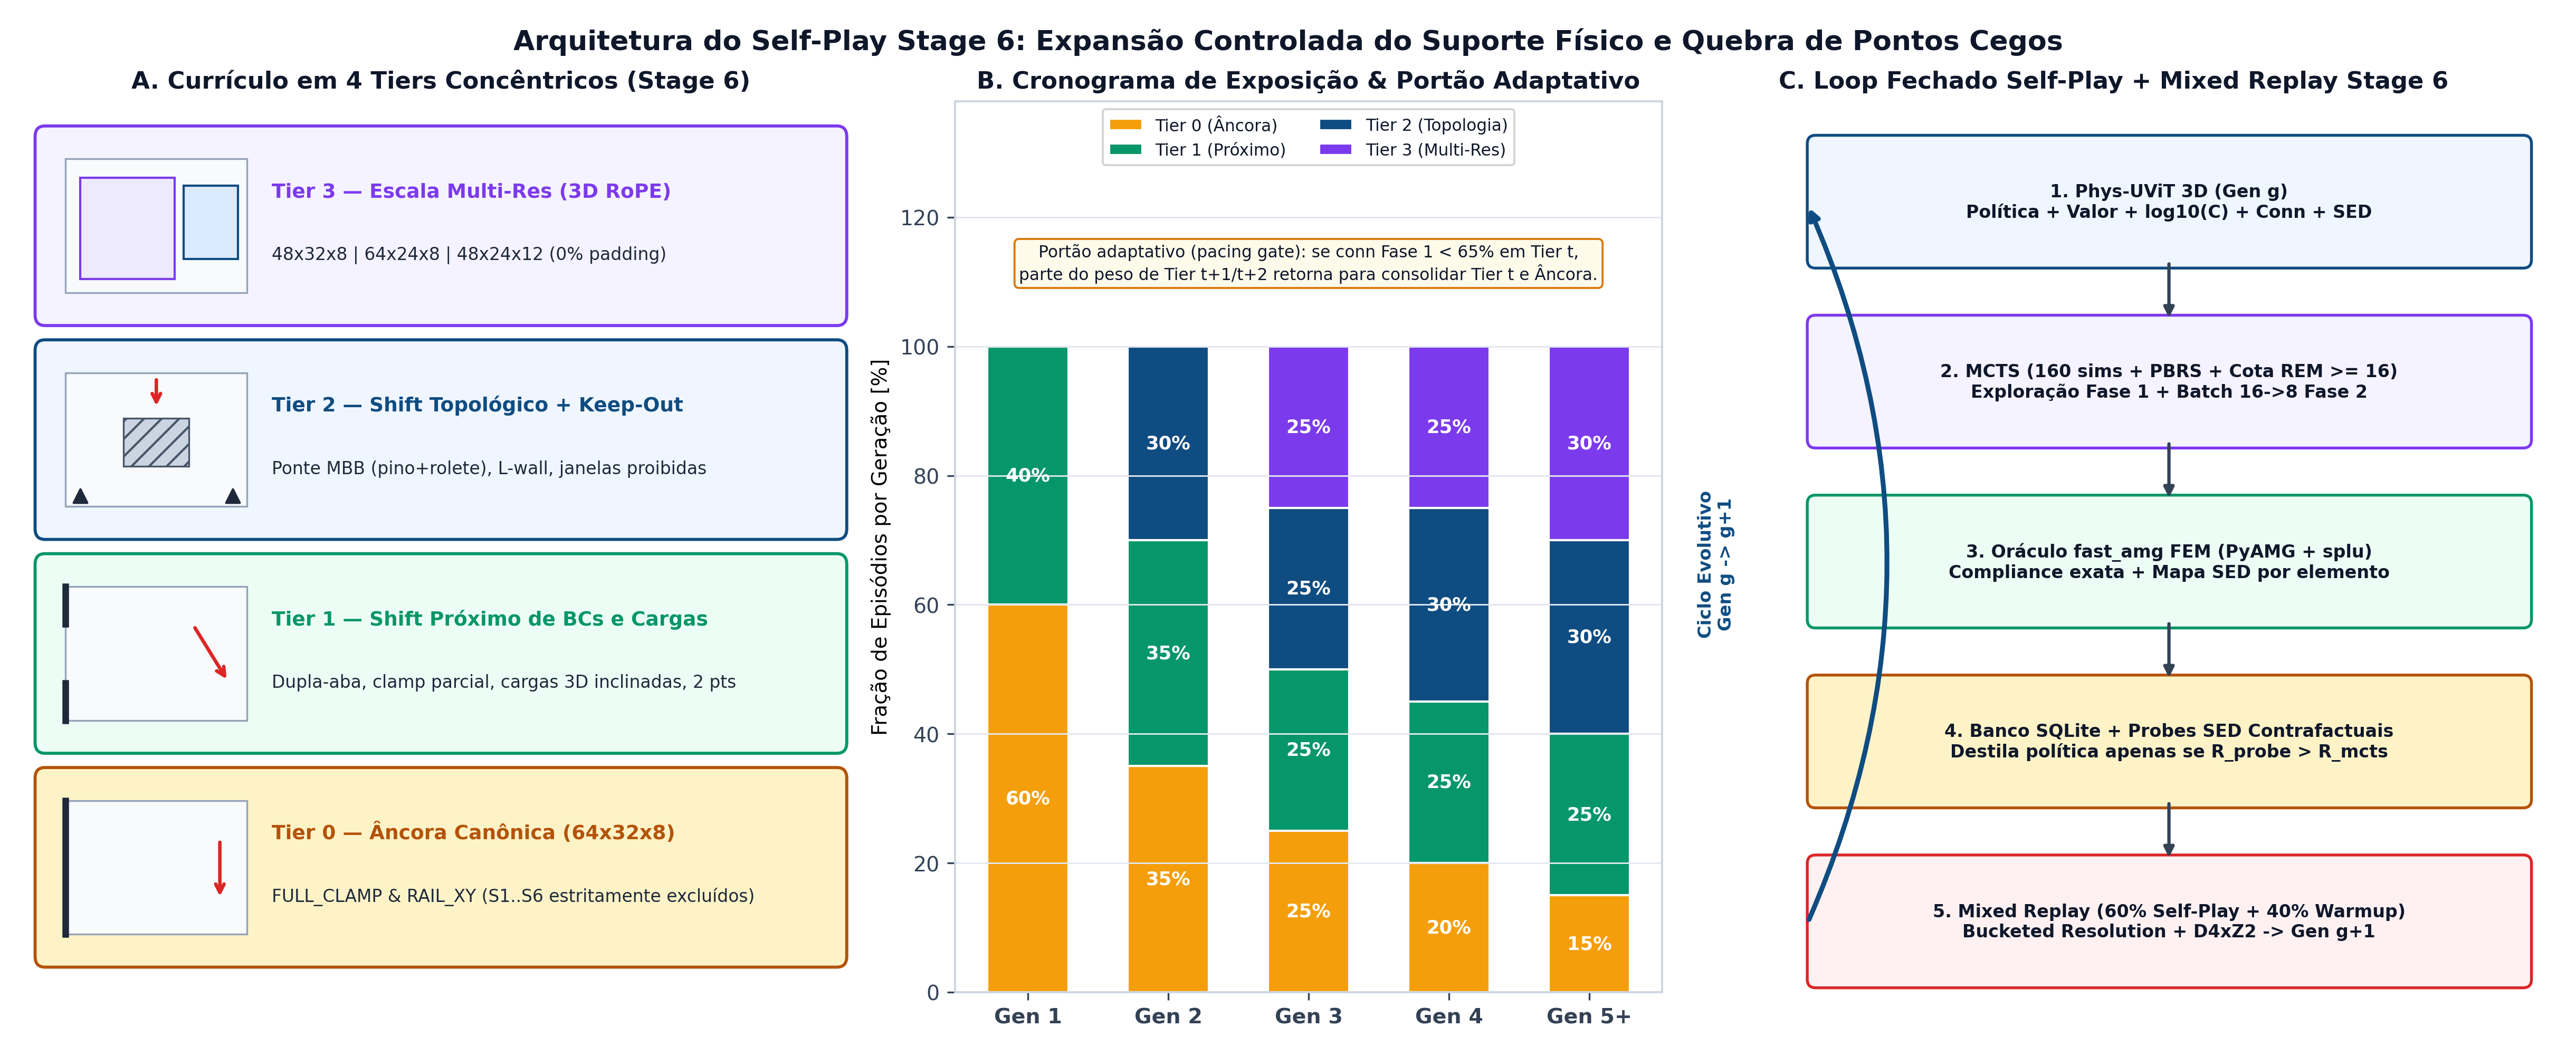
\includegraphics[width=\textwidth]{fig04_four_tier_curriculum_and_selfplay_loop.png}
\caption{Arquitetura completa do currículo em 4 Tiers concêntricos, cronograma de amostragem \texttt{Gen 1..5+} com portão adaptativo (\texttt{conn >= 65\%}) e ciclo evolutivo fechado com \texttt{fast\_amg} + \texttt{Mixed Replay}.}
\label{fig:stage6-arch}
\end{figure}

Cada anel introduz exatamente um novo grau de liberdade mecânica para que a rede generalize princípios estruturais universais sem perder a referência inicial:
\begin{enumerate}
\item \textbf{\texttt{Tier 0} — Âncora Canônica (\texttt{64x32x8}):} amostra engastes \texttt{FULL\_CLAMP} ($55\%$) e \texttt{RAIL\_XY} ($45\%$) com coordenadas $(x, y)$ variadas e excentricidades em $Z$, garantindo por \texttt{is\_near\_canonical\_scenario(..., tol\_xy=1)} que nenhuma vizinhança de \texttt{S1..S6} entre no treino. Mantém a rede ancorada na geometria de balanço padrão.
\item \textbf{\texttt{Tier 1} — Shift Próximo (\texttt{64x32x8}):} altera gradualmente o fluxo de esforços mantendo a grade $64\times 32\times 8$: engastes em dupla aba superior/inferior (\texttt{DUAL\_PAD\_CLAMP}) que quebram a simetria vertical do engaste contínuo sob cargas inclinadas no plano $XY$ ($\pm 25^\circ, \pm 35^\circ$), engastes centrais parciais (\texttt{PARTIAL\_CLAMP}) com componentes fora do plano $(f_y, f_z)$ induzindo flexo-torção 3D e carregamentos duplos simultâneos cuja resultante é normalizada.
\item \textbf{\texttt{Tier 2} — Shift Topológico e \emph{Keep-Out} (\texttt{64x32x8}):} rompe de vez os vícios de cantilever introduzindo \textbf{pontes bi-apoiadas MBB} (pino fixo em $x=0$ + rolete $U_y$ livre em $X$ na base $x=63$, onde a barra precisa formar um arco de compressão e cordão inferior de tração!), suportes em \textbf{L} (parede+piso) e cantilevers perfuradas por janelas vazias bloqueadas em \texttt{domain\_mask = 0}.
\item \textbf{\texttt{Tier 3} — Multi-Resolução via \texttt{3D RoPE}:} combina condições dos Tiers 0--2 sobre domínios \texttt{(48,32,8)}, \texttt{(64,24,8)} e \texttt{(48,24,12)} com $0\%$ de \emph{padding}. Em \texttt{48x24x12}, o gargalo Transformer passa de $Z=2$ para $Z=3$ tokens, validando se a atenção rotativa aprendeu elasticidade independente de proporção de caixa.
\end{enumerate}

\section{Exemplo Numérico do Portão Adaptativo (\texttt{adjust\_tier\_weights}) e Suíte OOD \texttt{G1..G4}}

O avanço de gerações segue os pesos da Tabela~\ref{tab:curriculum-sched}, mas submete-se ao \textbf{portão adaptativo (\texttt{adjust\_tier\_weights})}. Suponha que na \texttt{Gen 3}, cuja meta nominal é $(0.25,\, 0.25,\, 0.25,\, 0.25)$, a conectividade em Fase 1 do \texttt{Tier 1} ($t=1$) recue para $52\%$ ($< 65\%$). Em vez de prosseguir cegamente para pontes \texttt{MBB} e multi-resolução, o algoritmo transfere metade do peso do \texttt{Tier 2} ($0.5 \times 0.25 = 0.125$) e todo o peso do \texttt{Tier 3} ($0.25$), somando $\Delta w = 0.375$, e divide igualmente essa reserva de volta entre o \texttt{Tier 1} em dificuldade ($+0.1875 \to 43.75\%$) e a âncora \texttt{Tier 0} ($+0.1875 \to 43.75\%$), deixando \texttt{Tier 2} em $12.5\%$ e \texttt{Tier 3} em $0\%$.

Ao fim de cada geração (\texttt{scripts/run\_selfplay\_pipeline.py}), toda generalização é auditada por \textbf{MCTS puro (zero probes)} tanto em \texttt{S1..S6} ($30\times 8$ e estendido $64$) quanto na suíte OOD \texttt{G1..G4}: \texttt{G1\_dual\_pad\_angled} (carga a $30^\circ$), \texttt{G2\_bridge\_mbb} (ponte bi-apoiada), \texttt{G3\_keepout\_window} (janela proibida central $x\in[18,38), y\in[10,22)$) e \texttt{G4\_thick\_3d\_48x24x12} (bloco espesso com carga excêntrica em $Z$).

\begin{table}[htbp]
\centering
\caption{Cronograma progressivo de exposição nos 4 Tiers (\texttt{CURRICULUM\_SCHEDULE}).}
\label{tab:curriculum-sched}
\small
\begin{tabular}{@{}lcccc@{}}
\toprule
Geração & \texttt{Tier 0} (Âncora) & \texttt{Tier 1} (Próximo) & \texttt{Tier 2} (Topologia) & \texttt{Tier 3} (Multi-Res) \\
\midrule
\texttt{Gen 1} & $60\%$ & $40\%$ & $0\%$ & $0\%$ \\
\texttt{Gen 2} & $35\%$ & $35\%$ & $30\%$ & $0\%$ \\
\texttt{Gen 3} & $25\%$ & $25\%$ & $25\%$ & $25\%$ \\
\texttt{Gen 4} & $20\%$ & $25\%$ & $30\%$ & $25\%$ \\
\texttt{Gen 5+} & $15\%$ & $25\%$ & $30\%$ & $30\%$ \\
\bottomrule
\end{tabular}
\end{table}

\chapter{Fundamentação Preditiva, Leis de Escala e Matriz de Decisão}
\chaptermark{Fundamentação Preditiva e Matriz de Decisão}

\begin{notabox}{Distinção Estrita entre Fato Empírico e Projeção}
Os resultados até \texttt{Gen 0} (\texttt{ep19}: $+0.076$, $C_{\mathrm{S1}}=24{,}546$, \texttt{SIMP\_bin S6 = +0.048}, \texttt{SIMP\_cont} médio $+0.509$) e as testemunhas binárias em \texttt{dolfinx} ($C = 319.4$ e $356.4\text{ J}$) são \textbf{medições empíricas reais}. Os valores de \texttt{Gen 1..8} abaixo representam \textbf{projeções fundamentadas} em decomposição multiplicativa, com bandas Conservadora / Nominal / Otimista explícitas.
\end{notabox}

\section{Três Mecanismos pelos Quais Superaremos \texttt{SIMP\_bin} e \texttt{SIMP\_cont}}

\begin{enumerate}
\item \textbf{Margem já aberta sobre o \texttt{SIMP\_bin}:} a \texttt{Phys-UViT ep19} já vence \texttt{SIMP\_bin} em $6/6$ cenários ($+0.076$ contra $-0.825$ médio), porque respeita conectividade estrita $0/1$ em todo passo. Nos problemas \texttt{G1..G4} (pinos MBB e contornos de janela proibida), limiares contínuos rompem ainda mais rápido.
\item \textbf{Supressão do desperdício $\rho^3$ frente ao \texttt{SIMP\_cont}:} livre de densidades cinzentas sub-lineares, uma treliça ou viga caixão discreta $0/1$ obtém $100\%$ de $E_0$ por unidade de massa, permitindo menor compliance para a mesma massa — exatamente como demonstrado no \texttt{dolfinx} ($C=356.4$ e $319.4$ vs. $596.4\text{ J}$).
\item \textbf{Otimização direta sobre $R(C,V)$ em vez de restrição fixa de volume:} o \texttt{FEniTop} minimiza $C$ sujeito a um volume fixo ($V \approx 13$--$14.5\%$), enquanto o MCTS calibrado escolhe dinamicamente o ponto ótimo de Pareto onde o ganho de rigidez iguala a inclinação analítica $7.143$, podando voxels de baixo $\mathrm{SED}_e$ e reforçando apenas a linha de carga.
\end{enumerate}

\section{Convergência Multiplicativa, Compute e Critérios Promote/Hold/Kill}

\begin{figure}[htbp]
\centering
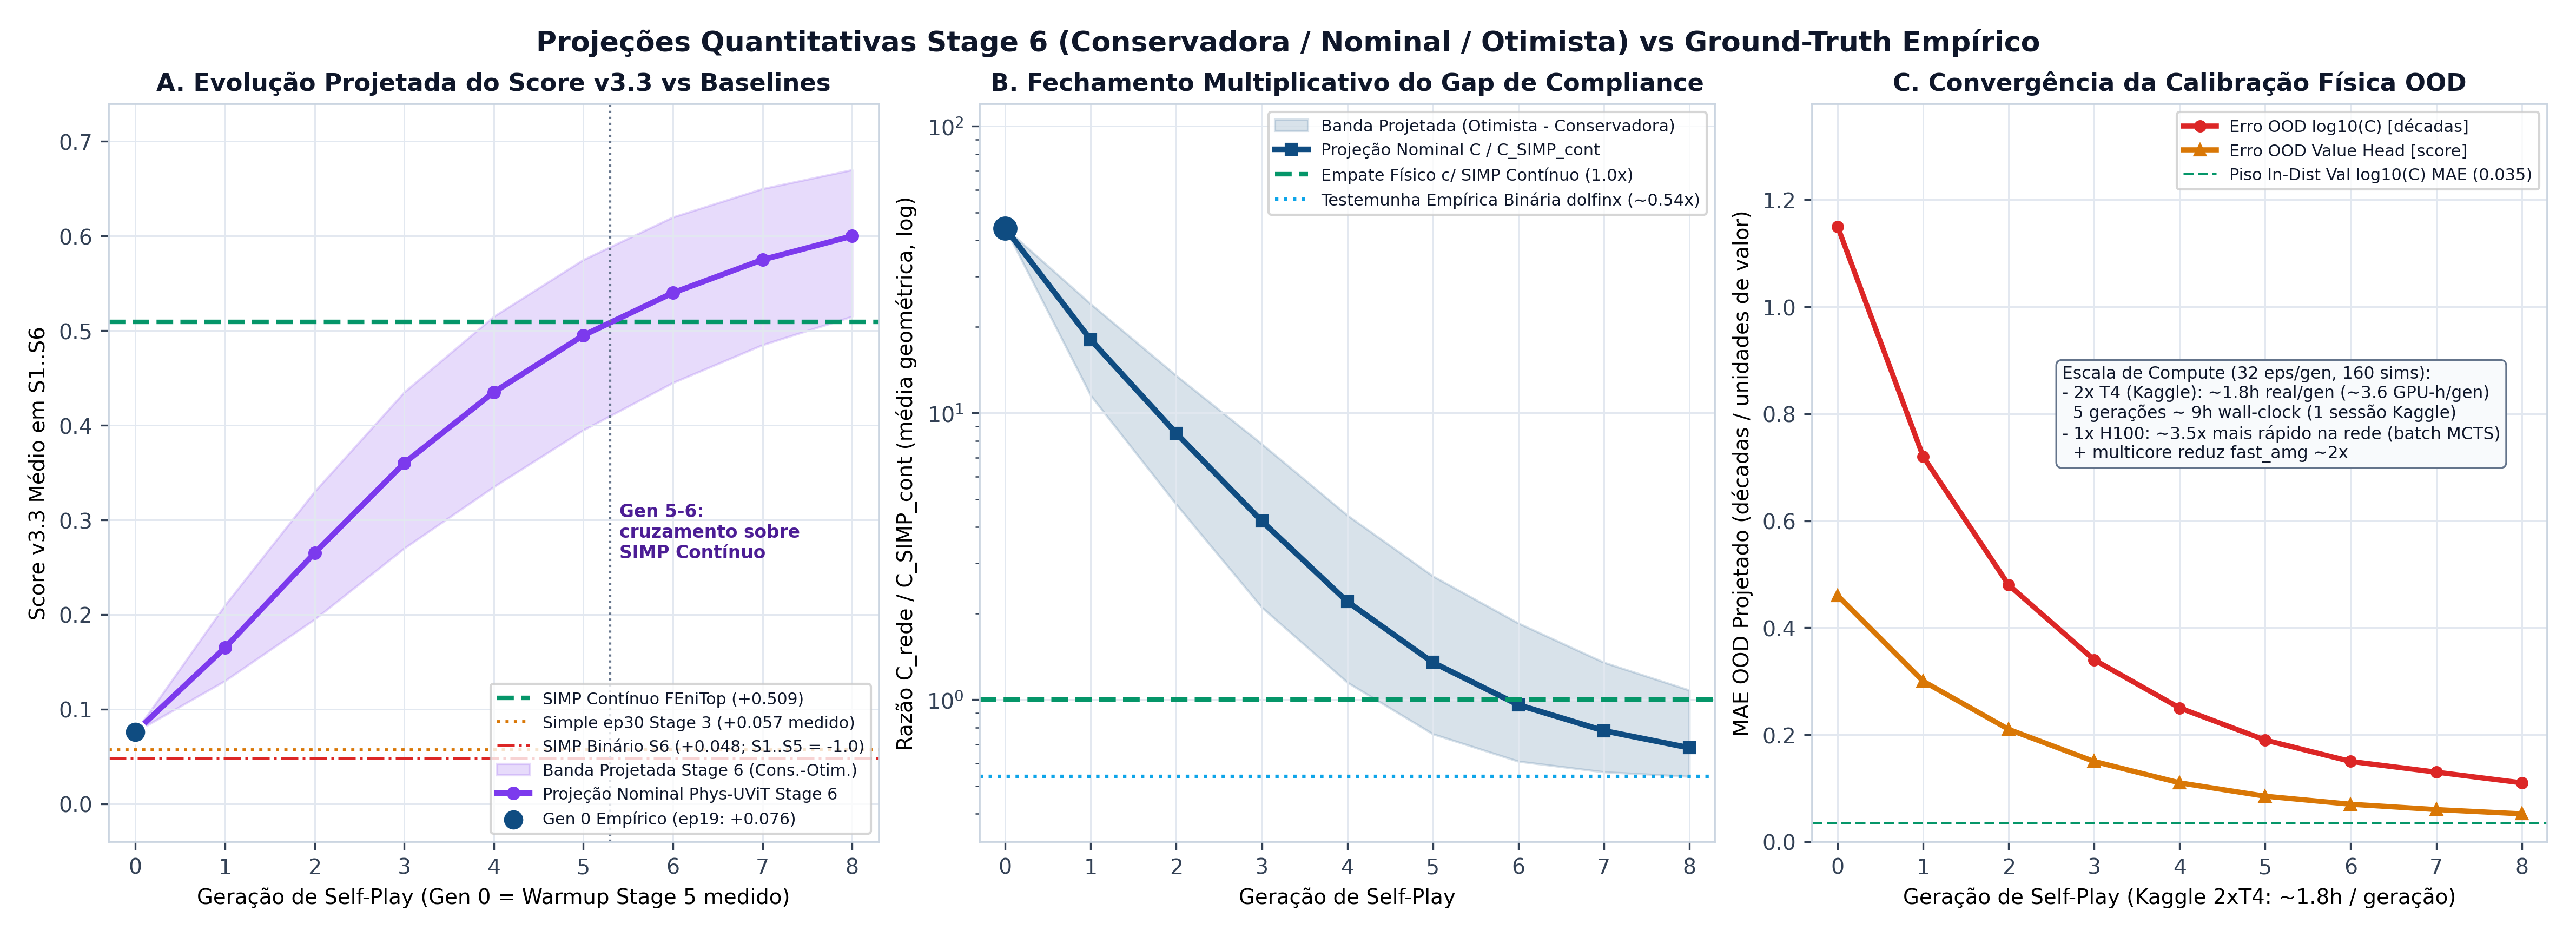
\includegraphics[width=\textwidth]{fig05_selfplay_projections_and_scaling_laws.png}
\caption{Projeções Stage 6 para Score \texttt{v3.3} médio (A), fechamento multiplicativo da razão $C / C_{\mathrm{SIMP\_cont}}$ até o teto empírico binário $\sim 0.54\times$ (B) e convergência da calibração OOD com orçamento computacional (C).}
\label{fig:projections}
\end{figure}

Decompondo os ganhos em três fatores multiplicativos independentes — redução do viés $\log_{10} C$ OOD ($\times 3$--$5$ em rigidez pela calibração + \texttt{SED}), abertura flexional $I_y$ por exploração em P1 + macro-lotes $16\to 8$ ($\times 4$--$8$) e cirurgia fina \texttt{REMOVE} guiada por \texttt{SED} ($\times 1.5$--$2.0$) —, o modelo cruza o patamar médio do \texttt{SIMP\_cont} ($+0.509$) nominalmente entre as gerações \textbf{5 e 6} (Figura~\ref{fig:projections} e Tabela~\ref{tab:projections}). Em um ambiente \texttt{2x Tesla T4} no Kaggle ($32$ episódios/gen, $160$ sims, \texttt{fast\_amg}), cada geração consome cerca de $1.8\text{h}$ reais ($\sim 3.6\text{ GPU-h/gen}$), permitindo rodar $4$--$5$ gerações completas dentro de uma única sessão sob guarda \texttt{--max-wall-hours 8.5}.

\begin{table}[htbp]
\centering
\caption{Projeções quantitativas Stage 6 (\texttt{S1..S6}) e escala computacional (\texttt{2x T4} vs. \texttt{H100}).}
\label{tab:projections}
\resizebox{\textwidth}{!}{%
\begin{tabular}{@{}lcccl@{}}
\toprule
Geração & Score \texttt{v3.3} (Cons. / Nom. / Otim.) & $C / C_{\mathrm{SIMP\_cont}}$ (Nom.) & OOD $\log_{10} C$ MAE & Marco Técnico e Decisão \\
\midrule
\texttt{Gen 0} (Medido) & $+0.076$ & $40.6\times$ & $1.10$--$1.15$ & Warmup Stage 5C (\texttt{ep19}, $0\%$ overshoot X) \\
\texttt{Gen 1} (Proj.) & $+0.130$ / $+0.165$ / $+0.210$ & $18.0\times$ & $\sim 0.72$ & Fim da correlação negativa em P2; primeiras remoções \\
\texttt{Gen 2} (Proj.) & $+0.195$ / $+0.265$ / $+0.330$ & $8.5\times$ & $\sim 0.48$ & Calibração P2 positiva; \texttt{Tier 2} ativo \\
\texttt{Gen 4} (Proj.) & $+0.335$ / $+0.435$ / $+0.515$ & $2.2\times$ & $\sim 0.25$ & Banzos profundos + multi-res \texttt{Tier 3} calibrada \\
\texttt{Gen 6} (Proj.) & $+0.445$ / $+0.540$ / $+0.620$ & $\mathbf{0.96\times}$ & $\sim 0.15$ & \textbf{Ultrapassagem nominal sobre \texttt{SIMP\_cont}} ($+0.509$) \\
\texttt{Gen 8} (Proj.) & $+0.515$ / $+0.600$ / $+0.670$ & $\mathbf{0.68\times}$ & $\sim 0.11$ & Consolidação plena em \texttt{S1..S6} e OOD \texttt{G1..G4} \\
\bottomrule
\end{tabular}%
}
\end{table}

\begin{mathbox}{Critérios Objetivos de Decisão por Geração no Kaggle}
\begin{itemize}
\item \textbf{PROMOVER:} se $\Delta\text{Score}(\texttt{S1..S6}) \ge +0.03$, erro OOD $\log_{10} C$ em queda e \texttt{conn(Tiers)} $\ge 70\%$, avançar para \texttt{Gen g+1}.
\item \textbf{MANTER / FREAR:} se \texttt{conn} em algum Tier cair $< 65\%$ ou \texttt{Blueprint Dice} em \texttt{Val-WU} recuar $> 2.5\%$, o portão adaptativo retém avanço e prioriza \texttt{Tier t} e âncora \texttt{Tier 0}.
\item \textbf{PARAR E DIAGNOSTICAR:} após duas gerações sem queda de \texttt{log10(C) OOD MAE} ou com estagnação persistente de Score, auditar razão \texttt{ADD/REM} e taxa de vitória dos \texttt{fem\_probes}.
\end{itemize}
\end{mathbox}

\appendix

\chapter{Runbook Operacional Kaggle \texttt{2 x Tesla T4} e Protocolo de Retomada}

Quando o orçamento semanal de GPUs do Kaggle for renovado, nenhuma alteração adicional no repositório é necessária:
\begin{enumerate}
\item Abrir \texttt{notebooks/alphabuilder-v4-stage6-selfplay.ipynb} em sessão Kaggle configurada com acelerador \texttt{GPU T4 x2} e Internet habilitada (apenas para instalar \texttt{pyamg==5.4.1}). O notebook localiza automaticamente \texttt{checkpoints/phys\_uvit\_v4\_stage5\_best.pt}, \texttt{warmup\_v3\_3\_kaggle.db} e \texttt{split\_v3\_3.json}.
\item O comando principal executa as gerações iniciais \texttt{1..5} distribuindo a coleta de $32$ episódios ($16$ por GPU) e sincronizando o ajuste fino via DDP com guarda segura de tempo limite (\texttt{--max-wall-hours 8.5}):
\begin{small}
\begin{verbatim}
python scripts/run_selfplay_pipeline.py \
  --init-checkpoint checkpoints/phys_uvit_v4_stage5_best.pt \
  --warmup-db data/kaggle_stage/warmup_v3_3_kaggle.db \
  --split-json data/kaggle_stage/split_v3_3.json \
  --work-dir outputs/stage6_selfplay \
  --start-gen 1 --end-gen 5 --gpus 2 \
  --episodes-per-gen 32 --num-simulations 160 \
  --p2-batch-early 16 --p2-batch-late 8 \
  --fem-backend fast_amg --selfplay-fraction 0.60 \
  --eval-extended --eval-ood --max-wall-hours 8.5
\end{verbatim}
\end{small}
\item Para continuar às gerações \texttt{6..8} em uma segunda sessão, basta exportar \texttt{outputs/stage6\_selfplay/} como Kaggle Dataset e passar \texttt{--resume-history outputs/stage6\_selfplay/selfplay\_evolution\_history.json --start-gen 6 --end-gen 8}, retomando diretamente do último checkpoint promovido e mantendo a janela deslizante de \emph{replay}.
\end{enumerate}

\chapter{Inventário dos Artefatos Stage 6 e Verificação Unitária}

\begin{table}[htbp]
\centering
\caption{Mapa completo dos arquivos criados/atualizados no Stage 6 e cobertos pela suíte \texttt{pytest} ($150$ aprovados).}
\label{tab:files-stage6}
\resizebox{\textwidth}{!}{%
\begin{tabular}{@{}ll@{}}
\toprule
Módulo / Script & Papel na Arquitetura Stage 6 \\
\midrule
\texttt{alphabuilder/src/logic/selfplay/fast\_fem.py} & Solver vetorizado \texttt{StructuredHex8FEM} (\texttt{BSR + PyAMG splu}) + mapa exato $\mathrm{SED}_e$ \\
\texttt{alphabuilder/src/logic/selfplay/evaluator.py} & Projeção Galerkin grau 2 no \texttt{dolfinx} + \texttt{bc\_masks/forces} generalizados \\
\texttt{alphabuilder/src/logic/mcts/\{node,engine,legal\_moves\}.py} & Cota \texttt{REMOVE >= 16} (\texttt{floor=0.25}) + bloqueio de \texttt{domain\_mask} \\
\texttt{alphabuilder/src/logic/selfplay/\{scenarios\_stage6,reward,runner,storage\}.py} & Tiers 0--3, exclusão \texttt{S1..S6}, portão $65\%$, \texttt{PBRS}, \texttt{fem\_probes} e merge SQLite \\
\texttt{alphabuilder/src/neural/\{selfplay\_dataset,dataset,trainer,inference\}.py} & \texttt{MixedReplayDataset} ($60/40$), \texttt{BucketedResolutionBatchSampler}, \texttt{sed\_loss} \\
\texttt{scripts/\{run\_selfplay\_pipeline,train\_selfplay\_step,evaluate\_inference\_scenarios\}.py} & Orquestrador multi-GPU, treino DDP e avaliação tripla (\texttt{S1..S6} + \texttt{G1..G4}) \\
\texttt{tests/unit/test\_stage6\_selfplay.py} \& \texttt{notebooks/alphabuilder-v4-stage6-selfplay.ipynb} & Suíte de paridade/dry-run verificada ($150$ aprovados) e notebook Kaggle pronto \\
\bottomrule
\end{tabular}%
}
\end{table}

\bibliographystyle{unsrtnat}
\bibliography{tcc/referencias}

\end{document}
